\documentclass[a4paper,twoside,11pt]{report} %openright
\newcommand{\documenttype}{Master Thesis}
\newcommand{\thesistitle}{Automated and Early Detection of Disease Outbreaks}
\newcommand{\thesissubtitle}{AEDDO}

\newcommand{\thesisauthor}{Kasper Schou Telkamp} % Your name :) 
\newcommand{\studentnumber}{s170397}
\newcommand{\thedate}{August, 2023} % For example "June, 2019"

\newcommand{\department}{DTU Compute}
\newcommand{\universitydescriber}{Technical University of Denmark}
\newcommand{\departmentdescriber}{Department of Applied Mathematics and Computer Science}
\newcommand{\sectiondescriber}{Section for Dynamical Systems}
\newcommand{\addressI}{Richard Petersens Plads, Building 324}
\newcommand{\addressII}{2800 Kgs. Lyngby}
\newcommand{\departmentwebsite}{www.compute.dtu.dk}


%\usepackage{microtype}      % better looking text
%\usepackage[utf8]{inputenc}
\usepackage{fontspec}       % Package for custom fonts
\usepackage[]{geometry}     % Package for changing page margins (before fancyhdr) 
\usepackage{fancyhdr}       % Package to change header and footer
\usepackage{parskip}        % Package to tweak paragraph skipping (instead of indents a small skip is added after every paragraph)
\usepackage{titlesec}
\usepackage{tikz}           % Package for drawing
\usepackage{pgfplots}       % Package for creating graphs and charts
\usepackage{xcolor}         % Package for defining DTU colours to be used
\usepackage{amsmath}        % For aligning equations among other
\usepackage{amssymb}
\usepackage{siunitx}        % SI units
\usepackage{listings}       % Package for inserting code, (before cleveref)
\PassOptionsToPackage{hyphens}{url} % Ability to line break urls at hyphens
\usepackage{hyperref}       % Package for cross referencing (also loads url package)
\usepackage{cleveref}       % improved cross referencing
\usepackage{textcomp}       % \textdegree = °C and other useful symbols
\usepackage[english]{babel} % localisation 
\usepackage{caption}        % better captions
\usepackage{subcaption}     % for subfigures
\usepackage{csquotes}       % For biblatex with babel
\usepackage[backend=biber,style=authoryear,sorting=none]{biblatex} % Package for bibliography (citing)
\bibliography{bibliography.bib}
\usepackage{tabularx}       % for ability to adjust column spacing in tabular better
\usepackage{tabu}
\usepackage{booktabs}       % for better tables
\usepackage{float}          % floating figures in correct places
\usepackage{calc}           % Adds ability for latex to calculate (3pt+2pt) 
%\usepackage[printwatermark=false]{xwatermark} % Package for wartermark. Toggle printwatermark true or false to include or remove the watermark
\usepackage{blindtext}
\usepackage{enumerate}
\usepackage{multirow}
\usepackage{longtable}
\usepackage[sort=none, abbreviations, postdot, stylemods, style=index]{glossaries-extra}


% Colours! 
\newcommand{\targetcolourmodel}{cmyk} % rgb for a digital version, cmyk for a printed version. Only use lowercase
\selectcolormodel{\targetcolourmodel}

% Define colours from https://www.designguide.dtu.dk/
\definecolor{dtured}    {rgb/cmyk}{0.6,0,0 / 0,0.91,0.72,0.23}
\definecolor{blue}      {rgb/cmyk}{0.1843,0.2431,0.9176 / 0.88,0.76,0,0}
\definecolor{brightgreen}{rgb/cmyk}{0.1216,0.8157,0.5098 / 0.69,0,0.66,0}
\definecolor{navyblue}  {rgb/cmyk}{0.0118,0.0588,0.3098 / 1,0.9,0,0.6}
\definecolor{yellow}    {rgb/cmyk}{0.9647,0.8157,0.3019 / 0.05,0.17,0.82,0}
\definecolor{orange}    {rgb/cmyk}{0.9882,0.4627,0.2039 / 0,0.65,0.86,0}
\definecolor{pink}      {rgb/cmyk}{0.9686,0.7333,0.6941 / 0,0.35,0.26,0}
\definecolor{grey}      {rgb/cmyk}{0.8549,0.8549,0.8549 / 0,0,0,0.2}
\definecolor{red}       {rgb/cmyk}{0.9098,0.2471,0.2824 / 0,0.86,0.65,0}
\definecolor{green}     {rgb/cmyk}{0,0.5333,0.2078 / 0.89,0.05,1,0.17}
\definecolor{purple}    {rgb/cmyk}{0.4745,0.1373,0.5569 / 0.67,0.96,0,0}

\newcommand{\dtulogocolour}{white} % Colour of the DTU logo: white, black or dtured
\newcommand{\frontpagetextcolour}{white} % front page text colour: white or black
\colorlet{frontbackcolor}{blue} % Set the background colour of the front- and back page. Choose the colour so it matches the main colour of front page picture

% DTU colours for diagrams
% You might want to make the front/back page background colour the first colour in the plot cycle list.
\pgfplotscreateplotcyclelist{DTU}{%
dtured,         fill=dtured,        \\%
blue,           fill=blue,          \\%
brightgreen,    fill=brightgreen    \\%
navyblue,       fill=navyblue       \\%
yellow,         fill=yellow         \\%
orange,         fill=orange         \\%
grey,           fill=grey           \\%
red,            fill=red            \\%
green,          fill=green          \\%
purple,         fill=purple         \\%
}


% Font
% There is no corporate serif font in the DTU design guide. The DTU design team has proposed to use Neo Sans for headings - and Arial for the body text.
% To change heading font to NeoSans Pro please upload both NeoSansPro-Regular.otf and NeoSansPro-Medium.otf to the root directory.
\setmainfont{Arial}
\renewcommand\thepart{Part \Roman{part}}
\IfFontExistsTF{NeoSansPro-Medium.otf}
{ %If True set headings to NeoSans Pro
\newfontface\NeoSansProReg{NeoSansPro-Regular.otf}
\newfontface\NeoSansProMed{NeoSansPro-Medium.otf}
\titleformat{\part}[display]{\NeoSansProMed \huge \centering}{\NeoSansProMed \Huge \thepart}{1em}{\thispagestyle{empty}}{}
\titleformat{\chapter}{\NeoSansProMed\huge}{\thechapter}{1em}{\raggedright}
\titleformat{\section}{\NeoSansProMed\Large}{\thesection}{1em}{\raggedright}
\titleformat{\subsection}{\NeoSansProMed\large}{\thesubsection}{1em}{\raggedright}
\titleformat{\subsubsection}{\NeoSansProMed\normalsize}{\thesubsubsection}{1em}{\raggedright}
\newcommand\TitleFont[1]{{\NeoSansProMed #1}}
\newcommand\titlefont[1]{{\NeoSansProReg #1}}
}
{ % If false
\titleformat{\part}[display]{\bfseries\huge \centering}{\bfseries\Huge \thepart}{1em}{\thispagestyle{empty}}{}
\titleformat{\chapter}{\bfseries\huge}{\thechapter}{1em}{\raggedright}
\titleformat{\section}{\bfseries\Large}{\thesection}{1em}{\raggedright}
\titleformat{\subsection}{\bfseries\large}{\thesubsection}{1em}{\raggedright}
\titleformat{\subsubsection}{\bfseries\normalsize}{\thesubsubsection}{1em}{\raggedright}
\newcommand\TitleFont[1]{{\bfseries #1}}
\newcommand\titlefont[1]{{#1}}
}
\urlstyle{sf}
%\def\UrlFont{\NeoSansProReg}


% If you wish to use the pdflatex compiler, sans-serif Helvetica can be used as a replacement for Arial. In this way you will be able to use the microtype package. Remember to add \usepackage[utf8]{inputenc} and disable the fontspec package. 
%\newcommand\TitleFont[1]{{\bfseries #1}}
%\newcommand\titlefont[1]{{#1}}
%\fontfamily{qhv}\selectfont
%\renewcommand{\familydefault}{\sfdefault}


% Watermark for confidential or draft (or anything else)
%\sffamily % set the correct font for the watermark
%\newsavebox\mybox
%\savebox\mybox{\tikz[color=grey,opacity=0.5]\node{Template};}

%\newwatermark*[
%  oddpages,
%  angle=60,
%  scale=12,
%  %fontfamily=qhv,
%  xpos=-40,
%  ypos=30,
%]{\usebox\mybox}

%\newwatermark*[
%  evenpages,
%  angle=60,
%  scale=12,
%  %fontfamily=qhv,
%  xpos=-50,
%  ypos=30,
%]{\usebox\mybox}


% Table of contents (TOC) and numbering of headings
\setcounter{tocdepth}{1}    % Depth of table of content: sub sections will not be included in table of contents
\setcounter{secnumdepth}{2} % Depth of section numbering: sub sub sections are not numbered

\makeatletter % Reset chapter numbering for each part
\@addtoreset{chapter}{part}
\makeatother  

% Spacing of titles and captions
\titlespacing\chapter{0pt}{0pt plus 4pt minus 2pt}{4pt plus 2pt minus 2pt}
\titlespacing\section{0pt}{12pt plus 3pt minus 3pt}{2pt plus 1pt minus 1pt}
\titlespacing\subsection{0pt}{8pt plus 2pt minus 2pt}{0pt plus 1pt minus 1pt}
\titlespacing\subsubsection{0pt}{4pt plus 1pt minus 1pt}{-2pt plus 1pt minus 1pt}
\captionsetup{belowskip=\parskip,aboveskip=4pt plus 1pt minus 1pt}

% Setup header and footer
\fancypagestyle{main}{% All normal pages
    \fancyhead{}
    \fancyfoot{}
    \renewcommand{\headrulewidth}{0pt}
    \fancyfoot[LE,RO]{\footnotesize \thepage}
    \fancyfoot[RE,LO]{\footnotesize \thesistitle} % - \rightmark
    \fancyhfoffset[E,O]{0pt}
}
\fancypagestyle{plain}{% Chapter pages
    \fancyhead{}
    \fancyfoot{}
    \renewcommand{\headrulewidth}{0pt}
    \fancyfoot[LE,RO]{\footnotesize \thepage}
    \fancyfoot[RE,LO]{\footnotesize \thesistitle} % - \leftmark
    \fancyhfoffset[E,O]{0pt}
}


% Setup for diagrams and graphs (tikz pictures) 
\usetikzlibrary{spy}    % For magnifying anything within a tikzpicture, see the line graph
\usepgfplotslibrary{statistics} % Package for the boxplot
\pgfplotsset{ % Setup for diagrams
compat=newest,
major x grid style={line width=0.5pt,draw=grey},
major y grid style={line width=0.5pt,draw=grey},
legend style={at={(0.5,-0.1)}, anchor=north,fill=none,draw=none,legend columns=-1,/tikz/every even column/.append style={column sep=10pt}},
axis line style={draw=none},
tick style={draw=none},
every axis/.append style={ultra thick},
tick label style={/pgf/number format/assume math mode}, % To apply main font to tick labels (numbers on the axis)
}
\tikzset{every mark/.append style={scale=1.5}}


% Hypersetup
\hypersetup{
    pdfauthor={\thesisauthor},
    pdftitle={\thesistitle},
    pdfsubject={\thesissubtitle},
    pdfdisplaydoctitle,
    bookmarksnumbered=true,
    bookmarksopen,
    breaklinks,
    linktoc=all,
    plainpages=false,
    unicode=true,
    colorlinks=false,
    hidelinks,                        % Do not show boxes or coloured links.
}


% Listings setup
\lstset{
    basicstyle=\footnotesize\ttfamily,% the size of the fonts that are used for the code
    commentstyle=\color{green},       % comment style
    keywordstyle=\bfseries\ttfamily\color{blue}, % keyword style
    numberstyle=\sffamily\tiny\color{grey}, % the style that is used for the line-numbers
    stringstyle=\color{purple},       % string literal style
    rulecolor=\color{grey},           % if not set, the frame-color may be changed on line-breaks within not-black text (e.g. comments (green here))
    breakatwhitespace=false,          % sets if automatic breaks should only happen at whitespace
    breaklines=true,                  % sets automatic line breaking
    captionpos=b,                     % sets the caption-position to bottom
    deletekeywords={},                % if you want to delete keywords from the given language
    escapeinside={\%*}{*)},           % if you want to add LaTeX within your code
    frame=single,                     % adds a frame around the code
    xleftmargin=4pt, 
    morekeywords={*,...},             % if you want to add more keywords to the set
    numbers=left,                     % where to put the line-numbers; possible values are (none, left, right)
    numbersep=10pt,                   % how far the line-numbers are from the code
    showspaces=false,                 % show spaces everywhere adding particular underscores; it overrides 'showstringspaces'
    showstringspaces=false,           % underline spaces within strings only
    showtabs=false,                   % show tabs within strings adding particular underscores
    stepnumber=1,                     % the step between two line-numbers. If it's 1, each line will be numbered
    tabsize=2,                        % sets default tabsize to 2 spaces
    title=\lstname,                   % show the filename of files included with \lstinputlisting; also try caption instead of title
}

% Signature field
\newlength{\myl}
\newcommand{\namesigdatehrule}[1]{\par\tikz \draw [black, densely dotted, very thick] (0.04,0) -- (#1,0);\par}
\newcommand{\namesigdate}[2][]{%
\settowidth{\myl}{#2}
\setlength{\myl}{\myl+10pt}
\begin{minipage}{\myl}%
\begin{center}
    #2  % Insert name from the command eg. \namesigdate{\authorname}
    \vspace{1.5cm} % Spacing between name and signature line 
    \namesigdatehrule{\myl}\smallskip % Signature line and a small skip
    \small \textit{Signature} % Text under the signature line "Signature"
    \vspace{1.0cm} % Spacing between "Signature" and the date line
    \namesigdatehrule{\myl}\smallskip % Date line and a small skip
    \small \textit{Date} % Text under date line "Date" 
\end{center}
\end{minipage}
}

% For the back page: cleartoleftpage
\newcommand*\cleartoleftpage{%
  \clearpage
  \ifodd\value{page}\hbox{}\newpage\fi
}


%Avoid shaded in RMarkdown
\usepackage{color}
\usepackage{fancyvrb}
\newcommand{\VerbBar}{|}
\newcommand{\VERB}{\Verb[commandchars=\\\{\}]}
\DefineVerbatimEnvironment{Highlighting}{Verbatim}{commandchars=\\\{\}}
% Add ',fontsize=\small' for more characters per line
\usepackage{framed}
\definecolor{shadecolor}{RGB}{248,248,248}
\newenvironment{Shaded}{\begin{snugshade}}{\end{snugshade}}
\newcommand{\AlertTok}[1]{\textcolor[rgb]{0.94,0.16,0.16}{#1}}
\newcommand{\AnnotationTok}[1]{\textcolor[rgb]{0.56,0.35,0.01}{\textbf{\textit{#1}}}}
\newcommand{\AttributeTok}[1]{\textcolor[rgb]{0.77,0.63,0.00}{#1}}
\newcommand{\BaseNTok}[1]{\textcolor[rgb]{0.00,0.00,0.81}{#1}}
\newcommand{\BuiltInTok}[1]{#1}
\newcommand{\CharTok}[1]{\textcolor[rgb]{0.31,0.60,0.02}{#1}}
\newcommand{\CommentTok}[1]{\textcolor[rgb]{0.56,0.35,0.01}{\textit{#1}}}
\newcommand{\CommentVarTok}[1]{\textcolor[rgb]{0.56,0.35,0.01}{\textbf{\textit{#1}}}}
\newcommand{\ConstantTok}[1]{\textcolor[rgb]{0.00,0.00,0.00}{#1}}
\newcommand{\ControlFlowTok}[1]{\textcolor[rgb]{0.13,0.29,0.53}{\textbf{#1}}}
\newcommand{\DataTypeTok}[1]{\textcolor[rgb]{0.13,0.29,0.53}{#1}}
\newcommand{\DecValTok}[1]{\textcolor[rgb]{0.00,0.00,0.81}{#1}}
\newcommand{\DocumentationTok}[1]{\textcolor[rgb]{0.56,0.35,0.01}{\textbf{\textit{#1}}}}
\newcommand{\ErrorTok}[1]{\textcolor[rgb]{0.64,0.00,0.00}{\textbf{#1}}}
\newcommand{\ExtensionTok}[1]{#1}
\newcommand{\FloatTok}[1]{\textcolor[rgb]{0.00,0.00,0.81}{#1}}
\newcommand{\FunctionTok}[1]{\textcolor[rgb]{0.00,0.00,0.00}{#1}}
\newcommand{\ImportTok}[1]{#1}
\newcommand{\InformationTok}[1]{\textcolor[rgb]{0.56,0.35,0.01}{\textbf{\textit{#1}}}}
\newcommand{\KeywordTok}[1]{\textcolor[rgb]{0.13,0.29,0.53}{\textbf{#1}}}
\newcommand{\NormalTok}[1]{#1}
\newcommand{\OperatorTok}[1]{\textcolor[rgb]{0.81,0.36,0.00}{\textbf{#1}}}
\newcommand{\OtherTok}[1]{\textcolor[rgb]{0.56,0.35,0.01}{#1}}
\newcommand{\PreprocessorTok}[1]{\textcolor[rgb]{0.56,0.35,0.01}{\textit{#1}}}
\newcommand{\RegionMarkerTok}[1]{#1}
\newcommand{\SpecialCharTok}[1]{\textcolor[rgb]{0.00,0.00,0.00}{#1}}
\newcommand{\SpecialStringTok}[1]{\textcolor[rgb]{0.31,0.60,0.02}{#1}}
\newcommand{\StringTok}[1]{\textcolor[rgb]{0.31,0.60,0.02}{#1}}
\newcommand{\VariableTok}[1]{\textcolor[rgb]{0.00,0.00,0.00}{#1}}
\newcommand{\VerbatimStringTok}[1]{\textcolor[rgb]{0.31,0.60,0.02}{#1}}
\newcommand{\WarningTok}[1]{\textcolor[rgb]{0.56,0.35,0.01}{\textbf{\textit{#1}}}}

\DeclareMathOperator{\E}{E}
\DeclareMathOperator{\V}{V}
\DeclareMathOperator{\G}{G}
\DeclareMathOperator{\N}{N}
\DeclareMathOperator{\NB}{NB}
\DeclareMathOperator{\ED}{ED}
\DeclareMathOperator{\Pois}{Pois}
\DeclareMathOperator{\Geom}{Geom}
\DeclareMathOperator*{\argmax}{arg\,max}
\DeclareMathOperator*{\argmin}{arg\,min}

\usepackage{amsthm}
\newtheorem{theorem}{Theorem}[chapter]
\newtheorem{lemma}{Lemma}[chapter]
\newtheorem{corollary}{Corollary}[chapter]
\newtheorem{proposition}{Proposition}[chapter]
\newtheorem{conjecture}{Conjecture}[chapter]
\theoremstyle{definition}
\newtheorem{definition}{Definition}[chapter]
\theoremstyle{definition}
\newtheorem{example}{Example}[chapter]
\theoremstyle{definition}
\newtheorem{exercise}{Exercise}[chapter]
\theoremstyle{definition}
\newtheorem{hypothesis}{Hypothesis}[chapter]
\theoremstyle{remark}
\newtheorem*{remark}{Remark}
\newtheorem*{solution}{Solution}
\begin{document}

\pagenumbering{roman}
\title{\thesistitle} 
\author{\thesisauthor} 
\date{\thedate} 

\begin{titlepage}

\newgeometry{left=11mm,right=11mm,top=50mm,bottom=0pt}
\pagecolor{frontbackcolor}
\color{\frontpagetextcolour}

{ % Thesis title (to change see Setup/Settings.tex) 
\Huge
\begin{tabular}{p{\linewidth}}
\TitleFont{\thesistitle}   \\ 
\TitleFont{\thesissubtitle} \bigskip \\ 
\titlefont{\documenttype}
\end{tabular}
}

% DTU department (to change see Setup/Settings.tex) 
\begin{tikzpicture}[remember picture,overlay]
\node[anchor=north east, 
      xshift=-10mm, 
      yshift=-12mm] 
      at (current page.north east) 
      {
        \color{\frontpagetextcolour}
        \begin{tabular}{r} 
        \textbf{\department} \\ 
        \departmentdescriber
        \end{tabular}
      }; 
\end{tikzpicture}

% DTU logo
\begin{tikzpicture}[remember picture,overlay]
\node[anchor=north west, 
      xshift=8.9mm, 
      yshift=-8.3mm] 
     at (current page.north west) 
     {\includegraphics[width=14.75mm,keepaspectratio]{Pictures/Logos/\dtulogocolour_\targetcolourmodel.pdf}}; 
\end{tikzpicture}

% Cover photo
\begin{tikzpicture}[remember picture,overlay]
\node[anchor=south, % anchor is bottom of picture
      xshift=0pt, 
      yshift=-2.9mm] % shifting picture to actually be at the bottom of the page
     at (current page.south) % placement at bottom of the page
     {
\includegraphics[height=18.9cm,keepaspectratio]{Pictures/DTU_stock_photo.jpg}};
\end{tikzpicture}




\end{titlepage}

\pagecolor{white}
\newgeometry{top=2.81cm, bottom=2.75cm, outer=2.5cm, inner=3.5cm}
\pagestyle{empty}
\cleardoublepage 
\thispagestyle{empty}
\setcounter{page}{1}
\vspace*{\fill}

\textbf{\thesistitle} \newline
\thesissubtitle

\smallskip

\documenttype \newline
\thedate

\smallskip

By \newline
\thesisauthor

\bigskip

\begin{tabularx}{\textwidth}{@{}lX@{}}
    Copyright: & Reproduction of this publication in whole or in part must include the customary bibliographic citation, including author attribution, report title, etc. \\
    Cover photo: & Vibeke Hempler, 2012 \\
    Published by: & DTU, \departmentdescriber, \addressI, \addressII ~Denmark  \\
     & \url{\departmentwebsite} \\
    ISSN: & [0000-0000] (electronic version) \\
    ISBN: & [000-00-0000-000-0] (electronic version) \\
    & \\
    ISSN: & [0000-0000] (printed version) \\
    ISBN: & [000-00-0000-000-0] (printed version)
\end{tabularx}



\clearpage 
\pagestyle{main}
\section*{Approval}
\addcontentsline{toc}{section}{Preface}
This thesis has been prepared over six months at the \sectiondescriber, \departmentdescriber, at the \universitydescriber, DTU, in collaboration with Epidemiologisk Forskning / Modelgruppen at Statens Serum Institut, SSI, in partial fulfilment for the degree Master of Science in Engineering, MSc Eng., Quantitative Biology and Disease Modelling. 

It is assumed that the reader has a basic knowledge in the areas of statistics. 

\vfill

\begin{center}
\namesigdate{\thesisauthor~-~\studentnumber}
\end{center}

\vfill


\clearpage 
\section*{Abstract}
\addcontentsline{toc}{section}{Abstract}

\blindtext






\clearpage 
\section*{Acknowledgements}
\addcontentsline{toc}{section}{Acknowledgements}

\textbf{Lasse Engbo Christiansen}, Senior Researcher, Statens Serum Institut \newline
\blindtext

\textbf{Jan Kloppenborg Møller}, Associate Professor, \universitydescriber \newline
\blindtext


\clearpage 
\section*{Notation}
\addcontentsline{toc}{section}{Notation}

The mathematical notation in this master's thesis is adapted from \cite{Madsen_2010}. All vectors are column vectors. Vectors and matrices are emphasized using a bold font. Lowercase letters are used for vectors and uppercase letters letters are used for matrices. Transposing is denoted with the upper index $^T$. Random variables are always written using uppercase letters. Thus, it is not possible to distinguish between a multivariate random variable and a matrix. However, variables and random variables are assigned to letters from the last part of the alphabet $(X, Y, Z, U, V, \dots)$, while constants are assigned to letters from the first part of the alphabet $(A, B, C, D, \dots)$. From the context it should be possible to distinguish between a matrix and a random vector.
\cleardoublepage 
\tableofcontents
\cleardoublepage 

%%%%%%%%%%%%%%%%%%%%%%%%%%%%%%%%%%%%%%%%%%%%%%%%%%%%%%%
\pagenumbering{arabic}
\chapter{Introduction}

This master's thesis will primarily focus on diseases where timely detection of outbreaks results in interventions that are feasible to impose. However, the detection algorithms discussed in this master's thesis are not restricted to these diseases and can be used to detect aberrant counts in any type of disease.

Today, outbreaks of foodborne illnesses can be detected in several ways:

\begin{enumerate}
  \item Reports from doctors: Physicians may report cases of foodborne illnesses they encounter in their practice to the relevant authorities.
  \item Citizen reports: Individuals may directly contact food or health authorities to report suspected cases of foodborne illnesses.
  \item Cluster identification through laboratory surveillance: Clusters of cases can be identified through routine laboratory testing and surveillance of samples from patients with suspected foodborne illnesses.
  \item Identification of identical "fingerprints": When bacteria or viruses are type-tested, the presence of identical fingerprints among multi cases can strongly indicate a common source of infection.
\end{enumerate}

These various methods help in the early detection and investigation of foodborne disease outbreaks, enabling timely intervention and prevention measures. However, \ldots{}

While generalized linear mixed effects models and hierarchical models have earned a reputation within \ldots, they are fairly unproven in the field of automatic detection of disease outbreaks.

The novel outbreak detection algorithms discussed in this master's thesis are open-source and can be found at \href{https://github.com/telkamp7/AEDDO}{https://github.com/telkamp7/AEDDO}

\cleardoublepage

\chapter{Setting the scene}

Outbreak investigations have a long history, dating back to John Snow's iconic removal of the handle of London's Broad Street pump during the cholera epidemic in 1865 \autocite{Tulchinsky_2018}. Indeed, while John Snow's work was groundbreaking for his time, modern disease outbreak investigations require more advanced and sophisticated techniques. Today, epidemiologists and public health professionals utilize a range of tools and methodologies to effectively tackle disease outbreaks. These may include advanced statistical analysis, mathematical modeling, molecular epidemiology \autocite{Honardoost_2018,Struelens_2013}, and whole-genome sequencing (WGS) \autocite{Koeser_2012,Baldry_2010}.

Meanwhile, the focus of this master's thesis is primarily on the field of advanced statistical analysis methods.

In recent years, there has been a notable increase in the interest surrounding statistical methods for automated and early detection of infectious disease outbreaks. These methodologies encompass a wide range of statistical techniques, including regression analysis, time series methodology, methods inspired by statistical process control, approaches incorporating spatial information, and multivariate outbreak detection. A comprehensive review of these methods can be found in \textcite{Buckeridge_2007} and \textcite{Unkel_2012}.

In addition to the aforementioned studies, state-of-the-art methods for aberration detection is presented in \textcite{Salmon_2016} and implemented in the R package called \textbf{surveillance}. The \textbf{surveillance} package provides various techniques for detecting aberrations in disease surveillance data, including the Farrington method initially introduced by \textcite{Farrington_1996} and subsequent improvements proposed by \textcite{Noufaily_2013}. These methods offer advanced statistical tools for detecting and monitoring disease outbreaks and are currently \textit{the} method choice at European public health institutes \autocite{Hulth_2010}.

Therefore, in this master's thesis, these established methods will be compared to a novel outbreak detection algorithm based on generalized mixed effects models and hierarchical generalized linear models respectively. The thesis introduces this new algorithm as an innovative approach to outbreak detection and aims to assess its performance in comparison to existing methods.

\cleardoublepage

\chapter{Surveillance data in Denmark}\label{Dataset}

This chapter delves into the data collection methods and quality assurance procedures within the Danish surveillance system. Moreover, it introduces the case studies selected for this master's thesis, which include \textit{Listeriosis}, \textit{Shigellosis}, Shiga toxin (verotoxin)-producing \textit{Escherichia coli} (STEC), and \textit{Salmonellosis}. These diseases will be referred to using either their full name or their related case definition:

\begin{itemize}
  \item LIST: \textit{Listeriosis}
  \item SHIG: \textit{Shigellosis}
  \item STEC: Shiga toxin (verotoxin)-producing \textit{Escherichia coli}
  \item SALM: \textit{Salmonellosis}
\end{itemize}

\section{Data collection and data quality}

In Denmark, the surveillance of infectious diseases is conducted by Statens Serum Institut (SSI). This surveillance system plays a pivotal role in national and international disease preparedness. It encompasses more than just the collection and registration of disease data; it also involves the prompt and ongoing dissemination of knowledge to the relevant authorities responsible for treatment, prevention, and control. This comprehensive approach ensures efficient communication and facilitates appropriate measures to address infectious diseases.

The quality of the Danish surveillance registers is maintained at a high standard, thanks to The National Board of Health Statutory Order on Physicians' Notification of Infectious Diseases (\href{https://www.retsinformation.dk/eli/lta/2000/277}{https://www.retsinformation.dk/eli/lta/2000/277}). This order specifies that several diseases\footnote{For a full list of diseases see \href{https://www.ssi.dk/sygdomme-beredskab-og-forskning/anmeldelse-af-sygdomme/lovpligtige-meldesystemer/individ_anmeldelses_sygdomme}{\nolinkurl{https://www.ssi.dk/sygdomme-beredskab-og-forskning/anmeldelse-af-sygdomme/lovpligtige-meldesystemer/individ_anmeldelses_sygdomme}}} are individually notifiable by physicians and general practitioners. Notifications consist of essential patient information and are submitted in paper form to both the Ministry of Health and to SSI. This rigorous notification process ensures accurate and comprehensive data collection for disease surveillance purposes in Denmark.

In addition to the individually notifiable diseases, SSI has implemented a laboratory notification system for numerous microorganisms. Clinical-microbiological laboratories are obligated to report the identification of specific microorganisms, along with relevant patient information. These data are then stored in the Danish Microbiology Database (MiBa), which was established by SSI in 2010. MiBa is a nationwide and automatically updated database specifically designed to collect and store microbiological test results. In order to utilize the data from MiBa, the information in the test results needs to have a standardized structure with common codes and terminology. MiBa employs national standards to harmonize the data, which initially may be structured in diverse formats. The standards currently used are XRPT05, which is widely employed for the exchange of microbiological test results in the healthcare system, and a specific standard called XRPT06. These standards are regularly revised and exist in various versions\footnote{Information on national standards and codes within the healthcare domain can be found on MedCom's website (\href{https://medcom.dk/}{https://medcom.dk/}).}. The national surveillance system focuses on diseases of a severe nature, those that are highly contagious, and the majority of vaccine-preventable diseases.

\section{Introducing the case studies}

For the scope of this master's thesis, only a specific subset of diseases from the mandatory notification system will be considered. This subset consists of \textit{Listeriosis}, \textit{Shigellosis}, Shiga toxin (verotoxin)-producing \textit{Escherichia coli} (STEC), and \textit{Salmonellosis}. These diseases have been chosen for analysis and investigation based on various factors, such as seasonality, incidence, and severity. Additionally, these diseases have been associated with documented outbreaks observed by SSI (\href{https://www.ssi.dk/sygdomme-beredskab-og-forskning/sygdomsudbrud/arkiv}{https://www.ssi.dk/sygdomme-beredskab-og-forskning/sygdomsudbrud/arkiv}) in the past decade, which adds to their relevance for the study.

The count observations are observed in the period from January 2008 to December 2022. An epidemic curve graph for an excerpt of the data for each of the diseases considered in this master's thesis is shown in Figure \ref{fig:EpiPlot}.



\begin{figure}[H]
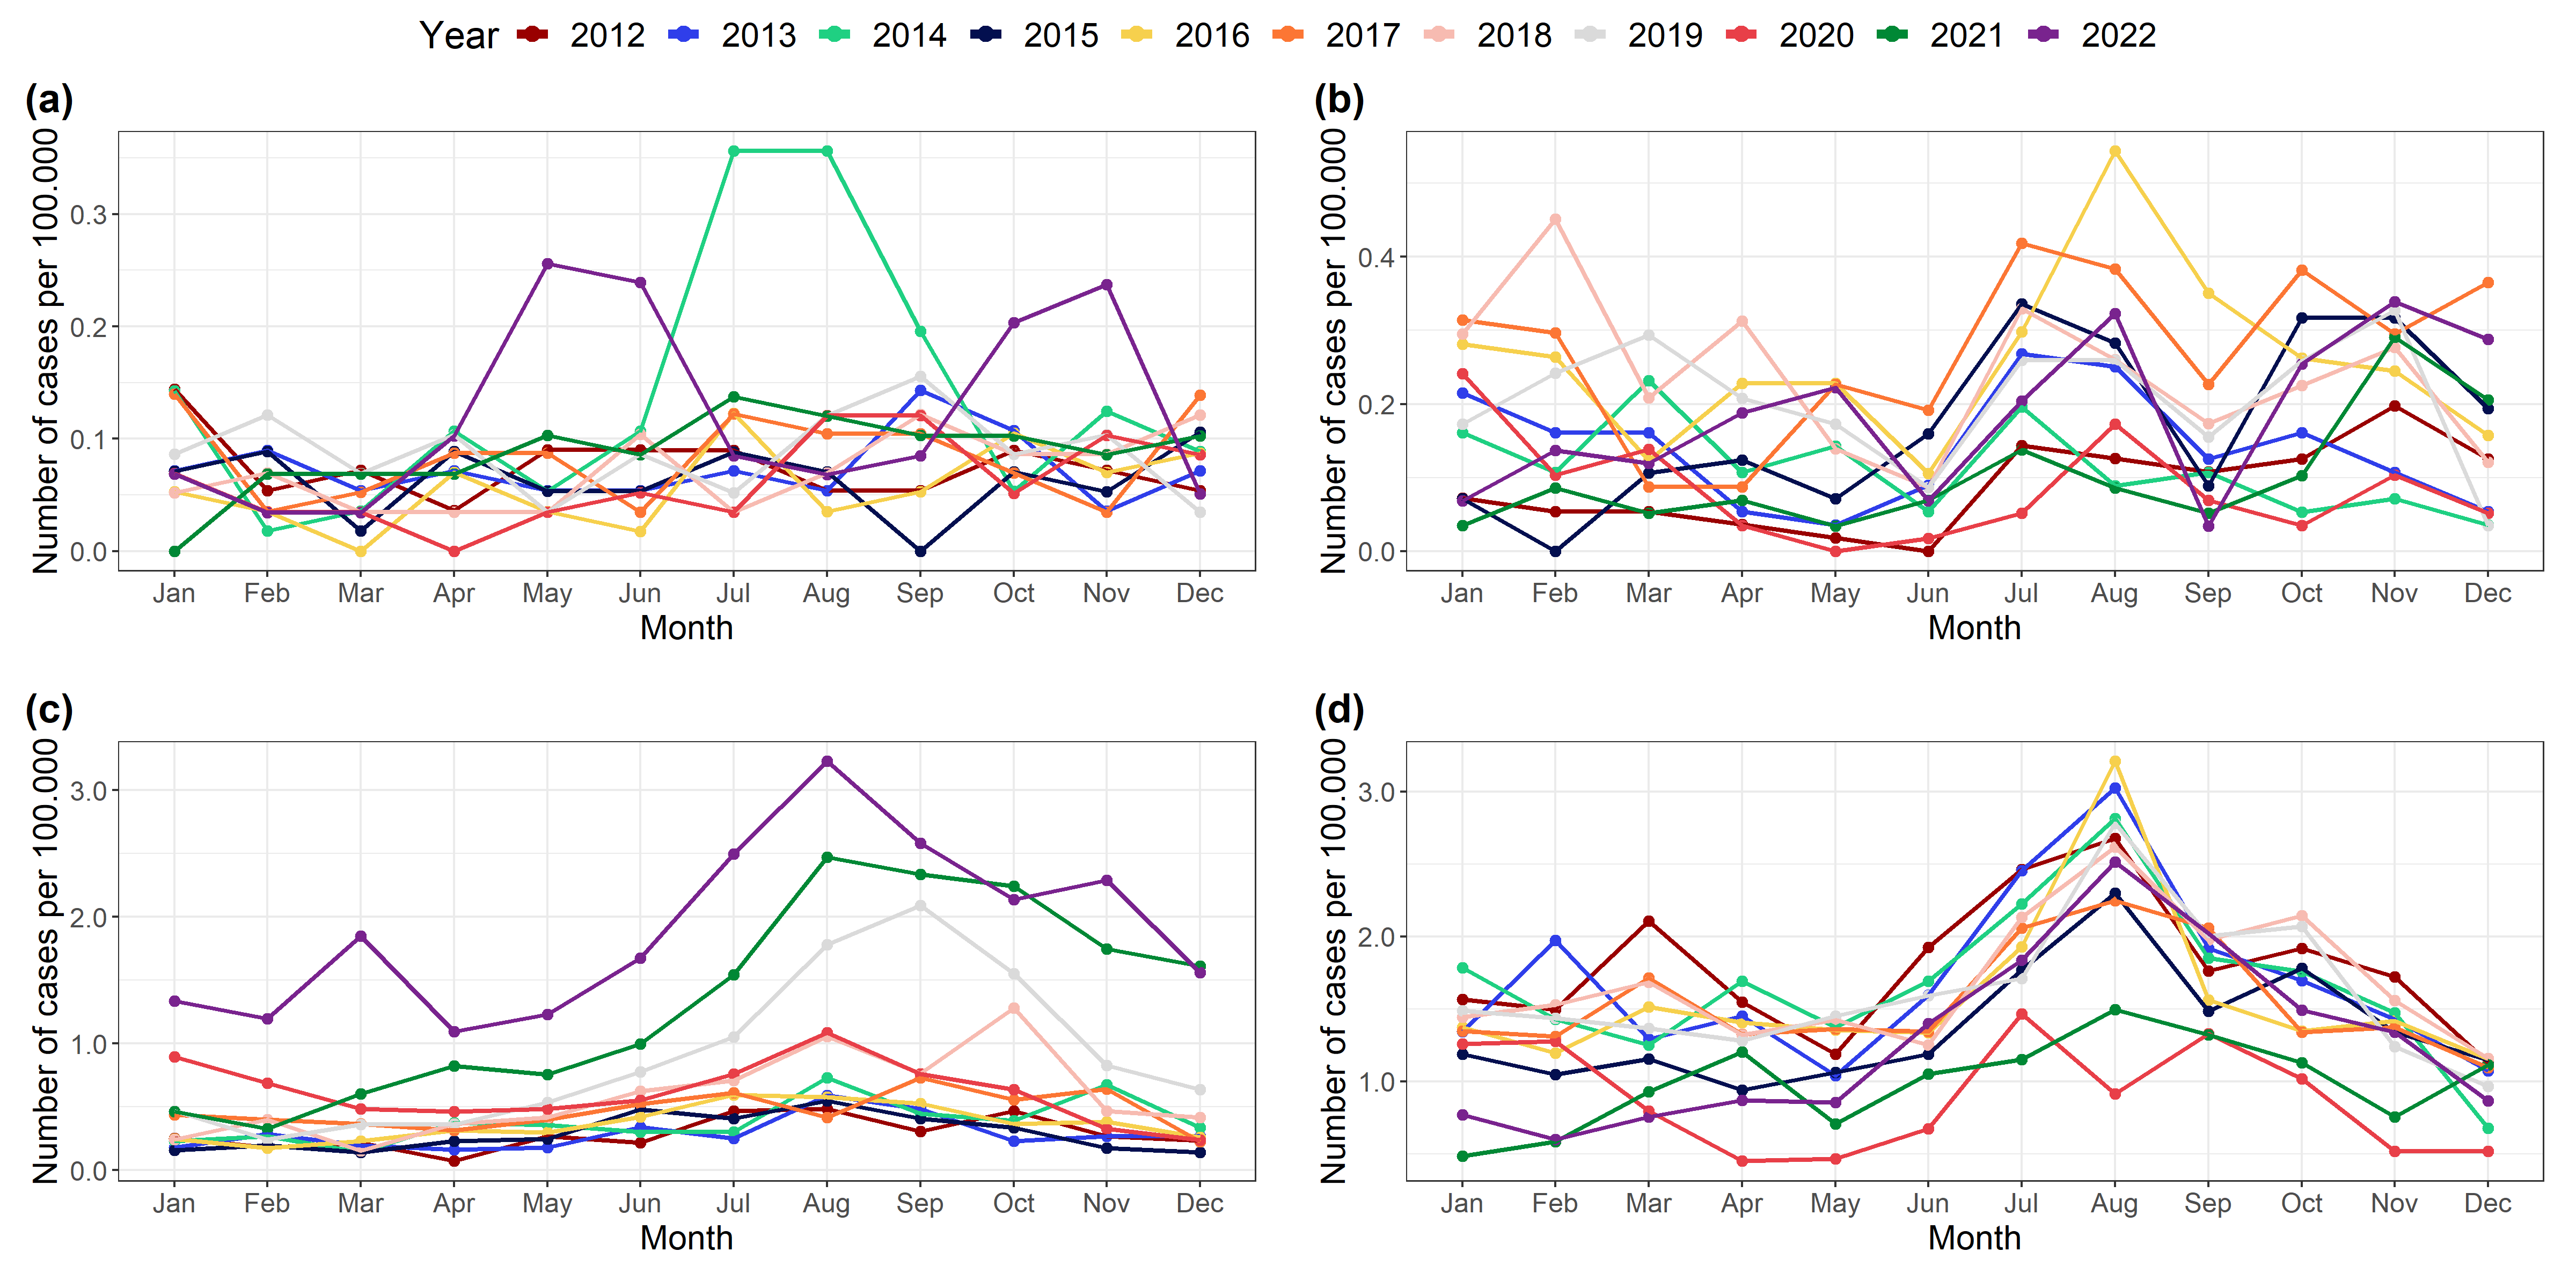
\includegraphics[width=1\linewidth]{../figures/EpiPlot} \caption{Epidemic curve showing the incidence per 100,000 in Denmark, 2012-2022, for the subset of diseases considered in this master thesis. \textbf{(a)} Listeriosis, \textbf{(b)} Shigellosis, \textbf{(c)} STEC, and \textbf{(d)} Salmonellosis.}\label{fig:EpiPlot}
\end{figure}

Evidently, the subset of diseases in Figure \ref{fig:EpiPlot} exhibits varying incidences and different levels of seasonal patterns on an annual basis. It is interesting to note that the incidences peak in August, which can be attributed to several factors, including:

\begin{itemize}
\item Increased travel activity: Especially when individuals travel to countries with unsafe drinking water, poor sanitation, and insufficient hygiene practices.
\item Large social gatherings: Events such as weddings, large festivals, or other gatherings where a significant number of people consume potentially contaminated food or drinking water.
\end{itemize}

Moreover, one could hypothesize that the warmer climate during the summer could potentially directly influence the proliferation of bacteria, which in turn may have an indirect impact on the transmission and spread of these diseases.

In general, there is a noticeable decrease in the number of observed cases starting from March 2020 and continuing until January 2021. This decline can be attributed to the strict lockdown measures implemented in Denmark in response to the Covid-19 pandemic. These measures, which involved restrictions on movement and social interactions, likely played a significant role in reducing the transmission of infectious diseases, including the ones being investigated.

In Figure \ref{fig:EpiPlot}a\ldots{}

In Figure \ref{fig:EpiPlot}b\ldots{}

Furthermore, in Figure \ref{fig:EpiPlot}c, a significant increase in the amplitude of the seasonal variation can be observed starting from 2018, with incidences doubling compared to the preceding years. At a first glance, this increase in the incidences might be recognized as a serious, reoccurring outbreak of the disease, but a more reasonable explanation can be found. Up to 2018, most departments of clinical microbiology used culture-based methods as a diagnostic test for bacterial pathogens and the process of changing the test method to polymerase chain reaction (PCR) methods was ongoing \autocite{Svendsen_2023}. In general, PCR resulted in higher incidences compared to other test methods, which is to no surprise as higher sensitivity is well documented for PCR \autocite{Buss_2015,Knabl_2016}.

Figure \ref{fig:EpiPlot}d \ldots{}

Some summary statistics for each of the disease considered in this master's thesis is gathered in Table \ref{tab:summaryStat}.

\begin{table}[H]

\caption{\label{tab:summaryStat}Summary statistics of the monthly count observations for the subset of diseases considered in this master's thesis. Boxplot: median (red line), IQR (grey box), whiskers (1.5 IQR), outliers (points).  Time series: normalized observations (0-1), first time points minimum and maximum count (red)}
\centering
\resizebox{\linewidth}{!}{
\begin{tabular}[t]{lrrrrr>{}l>{}l}
\toprule
Case definition & Min & Max & Mean & Median & Std. Deviation & Boxplot & Time series\\
\midrule
LIST & 0 & 20 & 4.446 & 4.0 & 2.934 & \includegraphics[width=0.67in, height=0.17in]{C:/GIT/AEDDO/Thesis/_main_files/figure-latex/boxplot_da436541bbd.pdf} & \includegraphics[width=0.67in, height=0.17in]{C:/GIT/AEDDO/Thesis/_main_files/figure-latex/plot_da4759723ab.pdf}\\
SHIG & 0 & 28 & 9.078 & 8.0 & 5.652 & \includegraphics[width=0.67in, height=0.17in]{C:/GIT/AEDDO/Thesis/_main_files/figure-latex/boxplot_da43e6b2293.pdf} & \includegraphics[width=0.67in, height=0.17in]{C:/GIT/AEDDO/Thesis/_main_files/figure-latex/plot_da429937941.pdf}\\
STEC & 2 & 80 & 21.933 & 16.5 & 14.902 & \includegraphics[width=0.67in, height=0.17in]{C:/GIT/AEDDO/Thesis/_main_files/figure-latex/boxplot_da422e61af8.pdf} & \includegraphics[width=0.67in, height=0.17in]{C:/GIT/AEDDO/Thesis/_main_files/figure-latex/plot_da41f06d20.pdf}\\
SALM & 0 & 583 & 108.012 & 85.5 & 82.725 & \includegraphics[width=0.67in, height=0.17in]{C:/GIT/AEDDO/Thesis/_main_files/figure-latex/boxplot_da424792676.pdf} & \includegraphics[width=0.67in, height=0.17in]{C:/GIT/AEDDO/Thesis/_main_files/figure-latex/plot_da469703be1.pdf}\\
\bottomrule
\end{tabular}}
\end{table}

In Table \ref{tab:summaryStat}, it is readily seen that the diseases exhibit different properties. WRITE SOME MORE!

All the diseases within the selected subset pose a significant risk of infection and can vary in terms of severity for affected individuals. Therefore, early identification of disease outbreaks is of utmost importance in order to promptly implement necessary interventions. Timely detection allows for swift and targeted actions to control the spread of these diseases and mitigate their impact on public health.

\subsection{\textit{Listeriosis}}

\textit{Listeriosis} is a foodborne illness that is caused by consuming food contaminated with \textit{Listeria monocytogenes}. This disease primarily affects pregnant women, unborn or newborn babies, the elderly, and individuals with weakened immune systems. \textit{Listeriosis} is associated with high mortality \autocite{Goulet_2012} and manifests in three ways: sepsis, meningitis, and mother-to-child transmission. Pregnancy-associated \textit{Listeriosis} can can have severe consequences for the fetus or newborn, including miscarriage, stillbirth, neonatal sepsis, and meningitis \autocite{Awofisayo_2015}. \textit{Listeriosis} is uncommon among individuals in other demographic groups. The bacteria is ubiquitous in the environment, found in moist environments, soil, water, decaying vegetation, and animals. Furthermore, it can survive and even grow under refrigeration and other food preservation measures.



\begin{figure}[H]
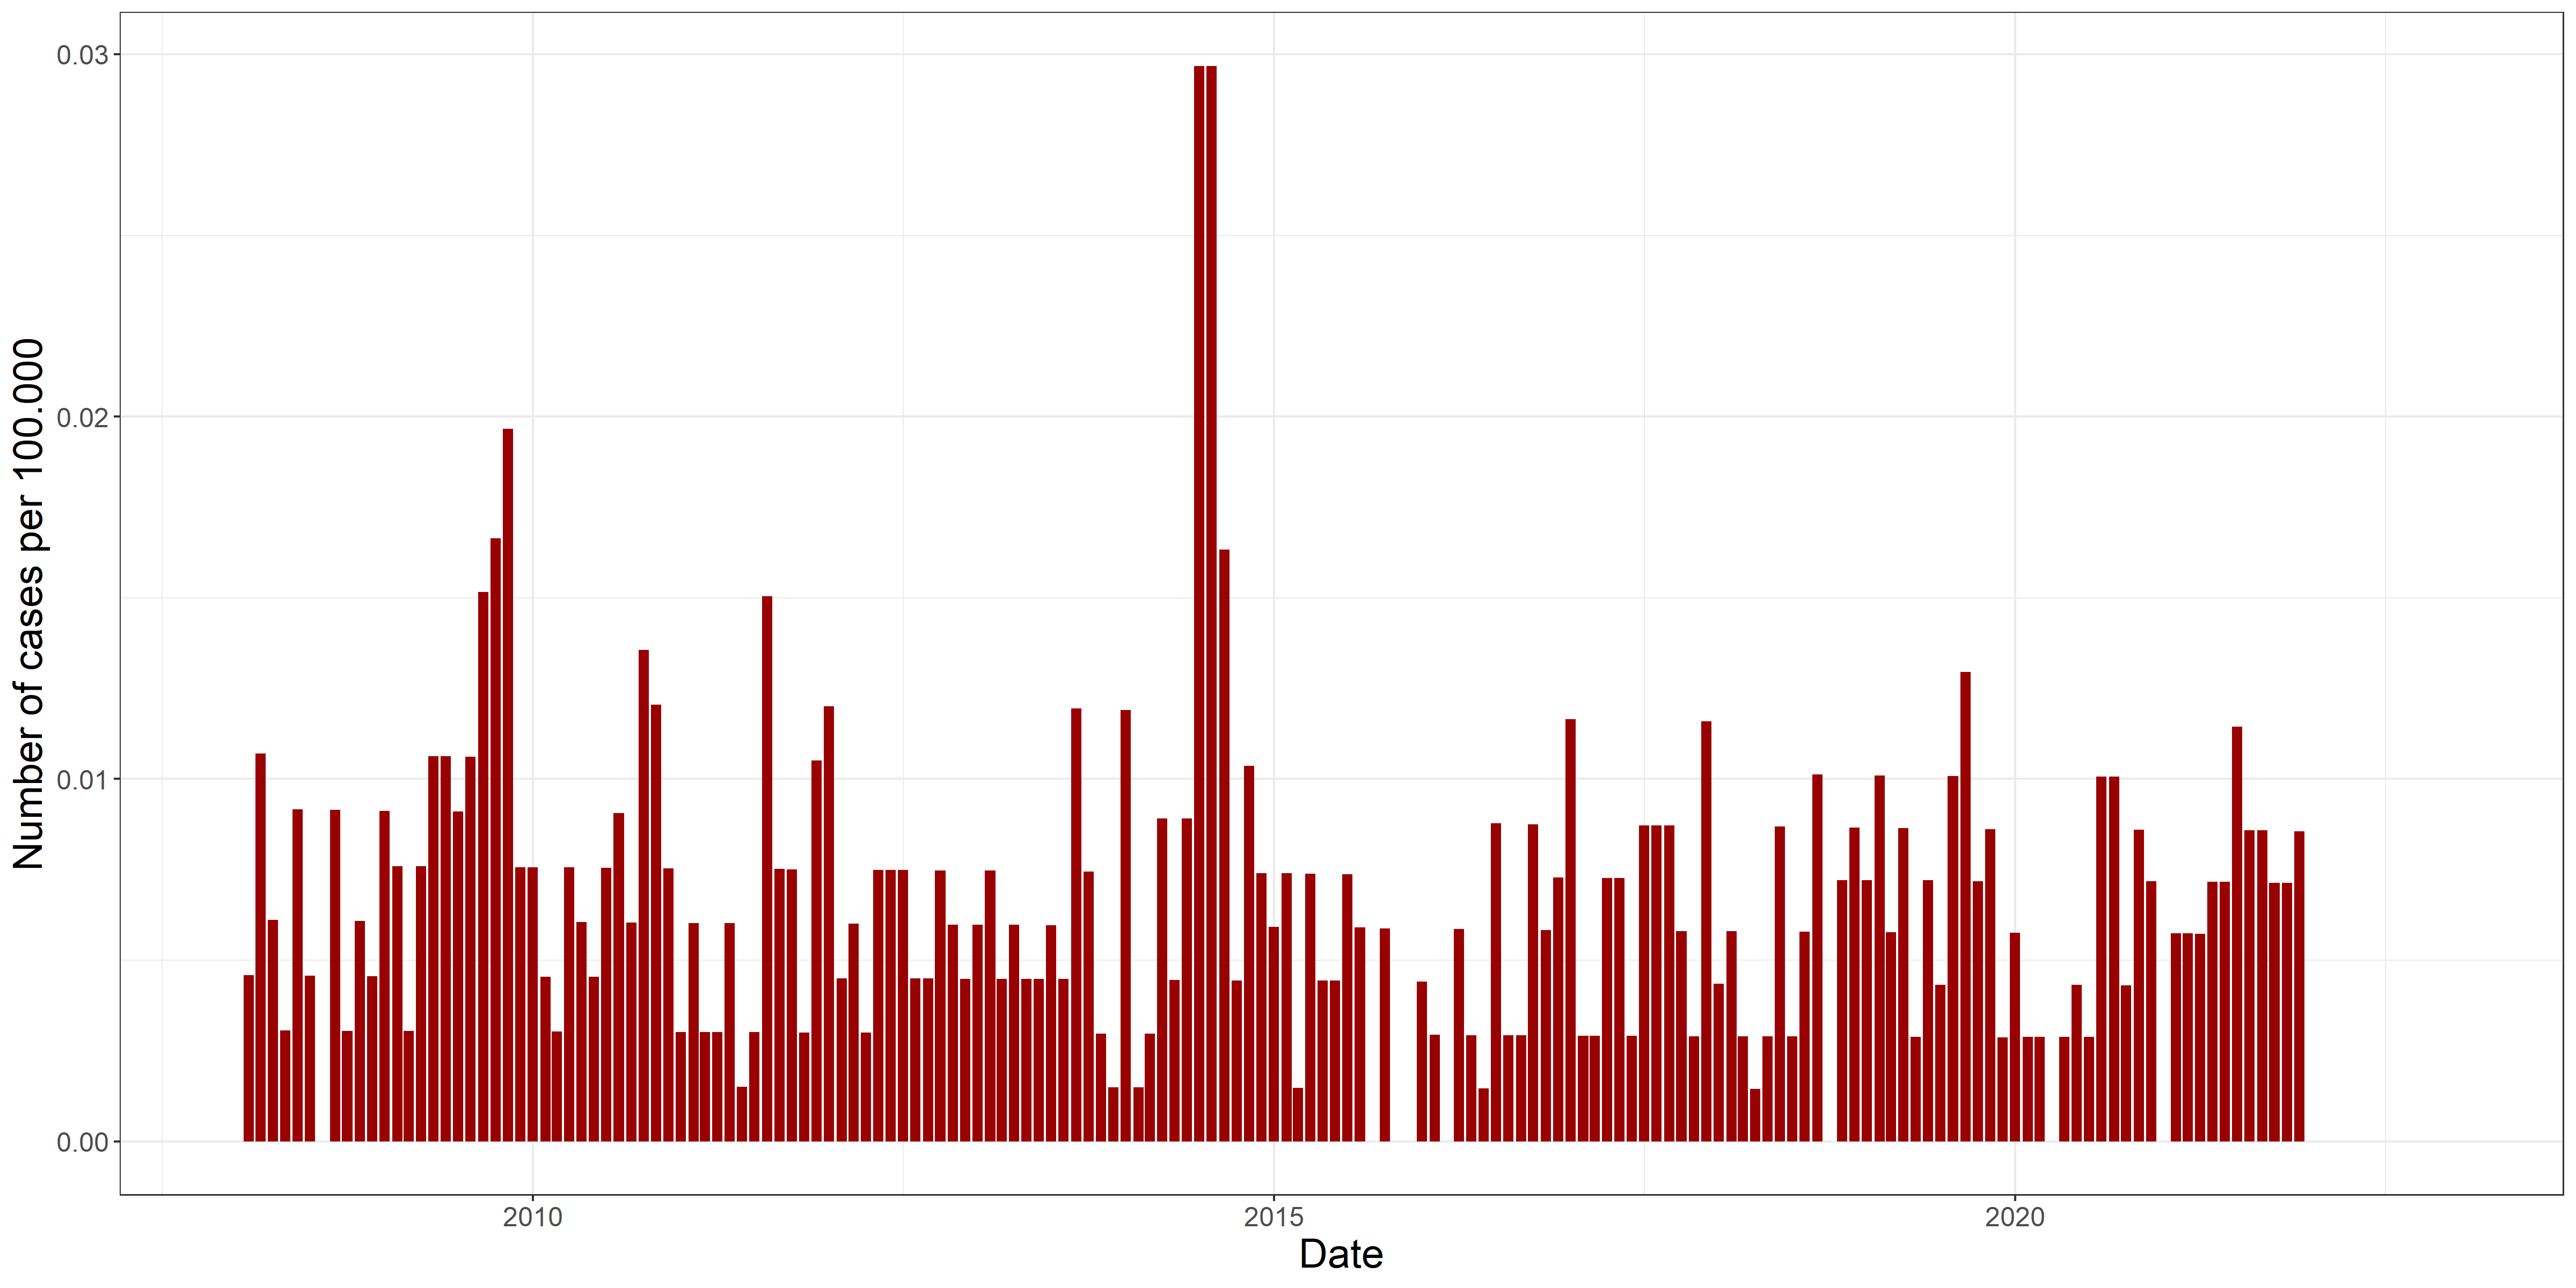
\includegraphics[width=1\linewidth]{../figures/LIST_long_plot} \caption{Placeholder caption}\label{fig:LISTLongPlot}
\end{figure}

In general, SSI employs whole-genome sequencing (WGS) as the state-of-the-art method to detect disease outbreaks caused by \textit{Listeria monocytogenes}. This method involves mapping the entire DNA of the bacteria and enables SSI to identify cases where patients are infected with identical Listeria bacteria. However, it is important to note that for this master's thesis, the DNA typing data is unavailable for use.

One notable outbreak investigated by SSI occurred between September 2013 and October 2014. This \textit{Listeriosis} outbreak involved a total of 41 cases, resulting in 17 deaths. Deli meat products from a specific company were identified as the source of the outbreak. The high mortality rate may be attributed to the consumption of these products in nursing homes and hospitals, where patients are more vulnerable. Following the discovery of Listeria at the facility, the Danish Veterinary and Food Administration recalled all products from the company.

In another \textit{Listeriosis} outbreak investigated by SSI, the source was traced back to cold-smoked and cured salmon products. A total of 5 related cases were identified, with 4 of them occurring in August 2017, and the fifth case in May 2017.

In some cases, despite extensive investigations, the source of contamination in an outbreak cannot always be identified. Such was the case in an unresolved outbreak that took place between the 13th of May and the 6th of June, 2022. During this period, a total of nine cases were infected with the same type of Listeria, with the majority of affected patients located in the Capital Region of Denmark. Despite thorough efforts, the specific source of contamination remained unknown.

Early identification of outbreaks caused by \textit{Listeria monocytogenes} is crucial to implement timely interventions and mitigate the impact of the disease. Otherwise, these outbreaks can persist over an extended period. SSI has successfully resolved several long-spanned outbreaks in the last decade. For example, one investigation revealed that a single outbreak was actually two simultaneous outbreaks caused by the consumption of smoked fish. Each outbreak consisted of ten cases and spanned from May 2013 to July 2015 \autocite{Gillesberg_2016}.

Other documented long-spanned outbreaks investigated by SSI include:

\begin{itemize}
  \item A cold-smoked fish outbreak with 9 cases spanning from December 2016 to February 2019.
  \item A prolonged outbreak with 6 cases from 2016 to 2019, traced back to a local greengrocer.
  \item An outbreak with 8 cases from October 2021 to June 2022, caused by a deli meat product.
  \item Two unresolved outbreaks with 9 cases and 12 cases from the end of 2018 to November 2021 and October 2020 to May 2022, respectively.
\end{itemize}

The use of WGS in these outbreaks provided the ability to link cases that occurred over a period of years and revealed that they were, in fact, continuous-source outbreaks.

In a recent outbreak investigated by SSI, the Danish Veterinary and Food Administration, and the National Food Institute at the Technical University of Denmark, fish patties were identified as the source of contamination. This outbreak occurred from August 2022 to December 2022 and affected a total of 11 cases.



\begin{figure}[H]
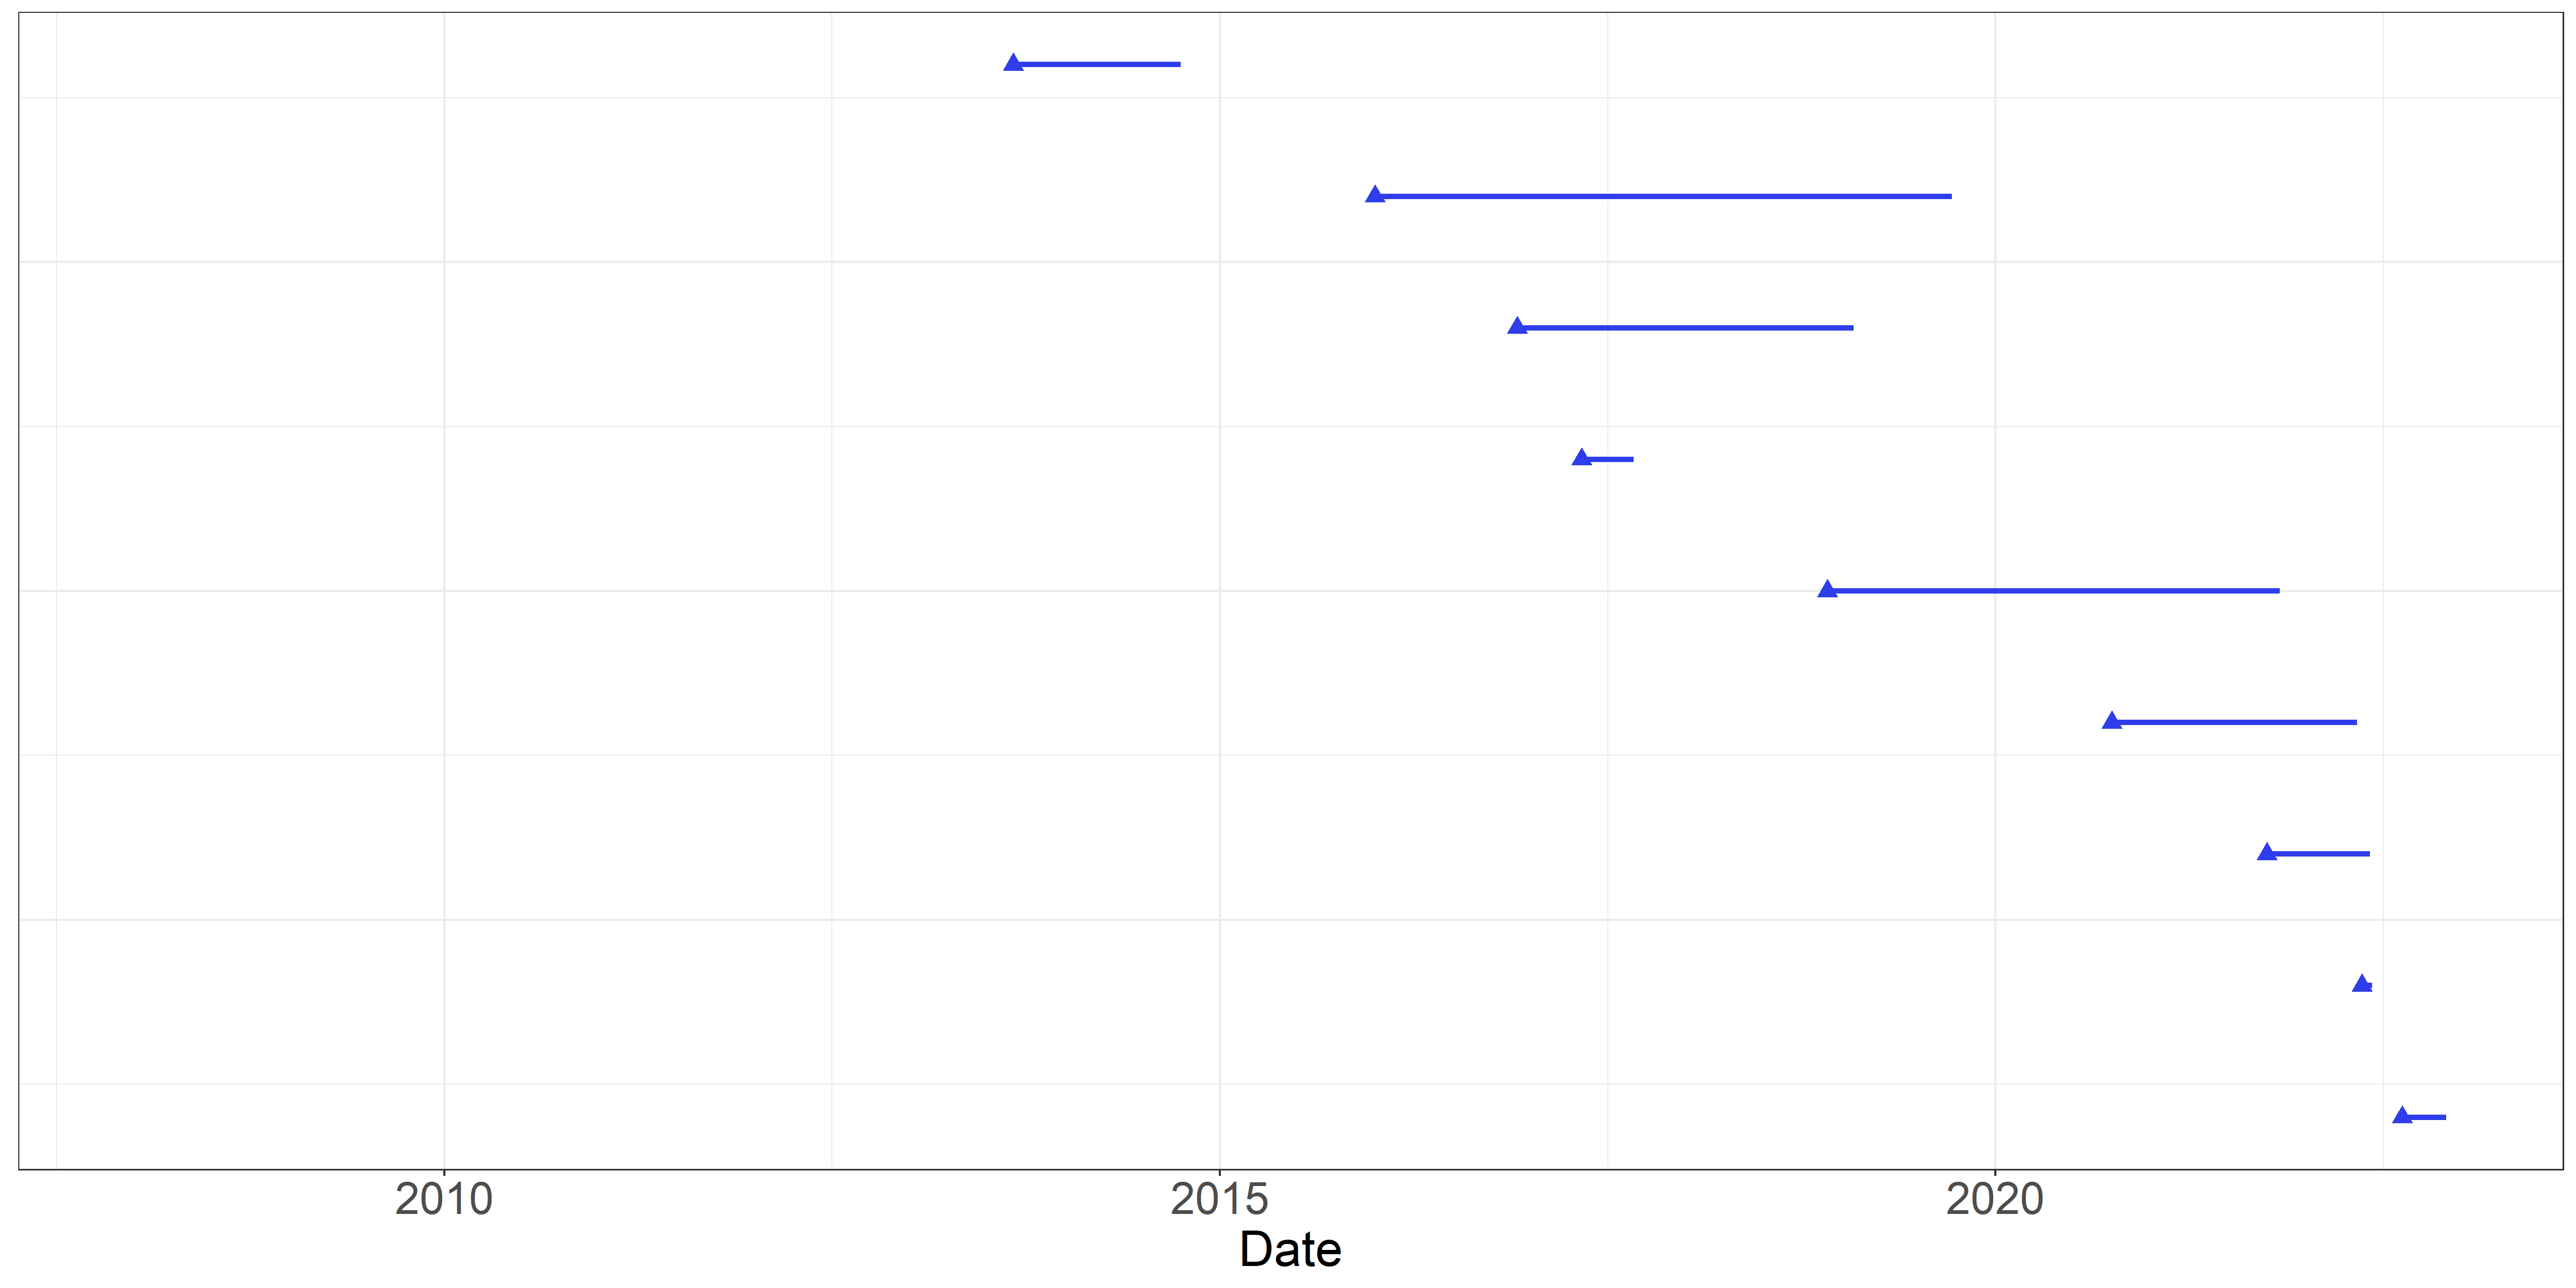
\includegraphics[width=1\linewidth]{../figures/LIST_SSI_outbreaks} \caption{Timeline indicating the start (triangle) and duration (line) of documented outbreaks of \textit{Listeriosis} by SSI and possible collaborators.}\label{fig:LISTSSIoutbreaks}
\end{figure}

\subsection{\textit{Shiggellosis}}

\textit{Shiggellosis} is a diarrheal illness that is caused by a group of bacteria called \textit{Shigella}. The bacteria are highly contagious and can be transmitted through direct person-to-person contact, consumption of contaminated food, or ingestion of water contaminated with human feces. \textit{Shigella} infections are most commonly observed in children under the age of 5, individuals traveling to regions with poor sanitation and unsafe water and food practices, as well as gay, bisexual, and other men who have sex with men.



\begin{figure}[H]
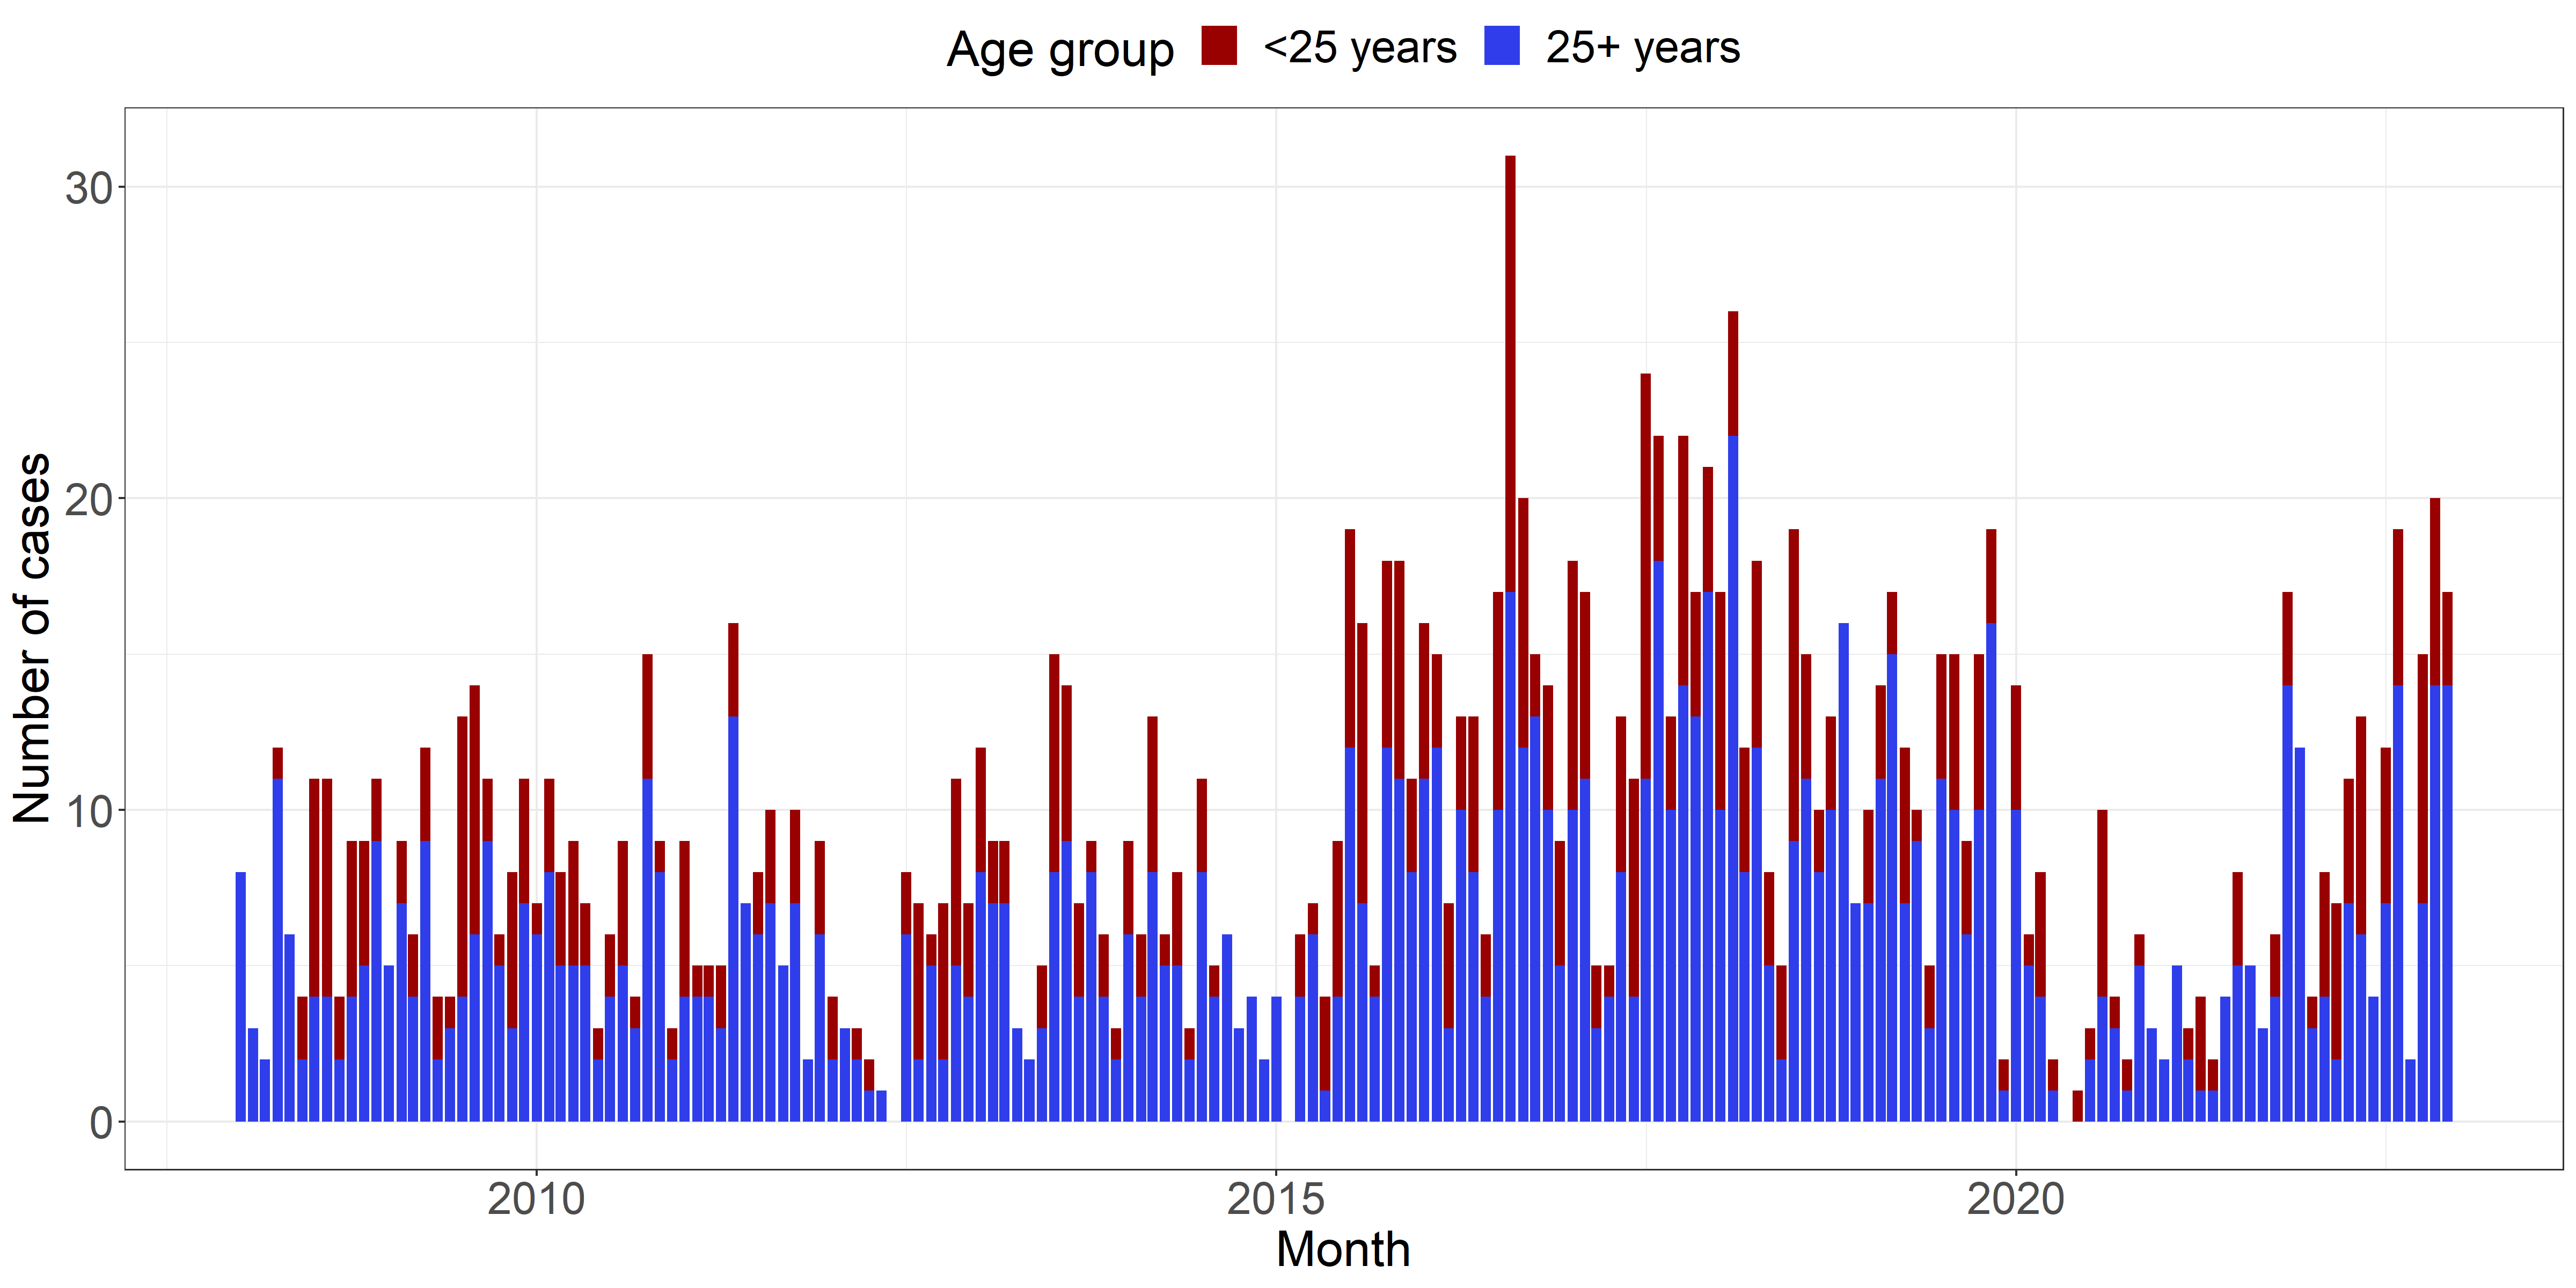
\includegraphics[width=1\linewidth]{../figures/SHIG_long_plot} \caption{Placeholder caption}\label{fig:SHIGLongPlot}
\end{figure}

In Denmark, another significant cause of \textit{Shigellosis} outbreaks is the importation of contaminated vegetables. This was evident in several incidents, including a 2007 outbreak where 215 individuals fell ill after consuming imported contaminated baby corn \autocite{Lewis_2009,Muller_2009}, a smaller outbreak in 2009 linked to sugar snap peas from Kenya, and a 2020 outbreak associated with fresh mint as the source of infection.

The 2020 outbreak is indeed a significant focus of this study, as it serves as a benchmark for evaluating the effectiveness of outbreak detection algorithms. It took place from the 22th of August to the 9th of September and was investigated by SSI in collaboration with the Danish Veterinary and Food Administration and the National Food Institute at the Technical University of Denmark. The outbreak affected 44 patients, mainly concentrated in the Capital Region of Denmark. During the investigation, at least five events were identified where individuals subsequently developed \textit{Shigellosis}.



\begin{figure}[H]
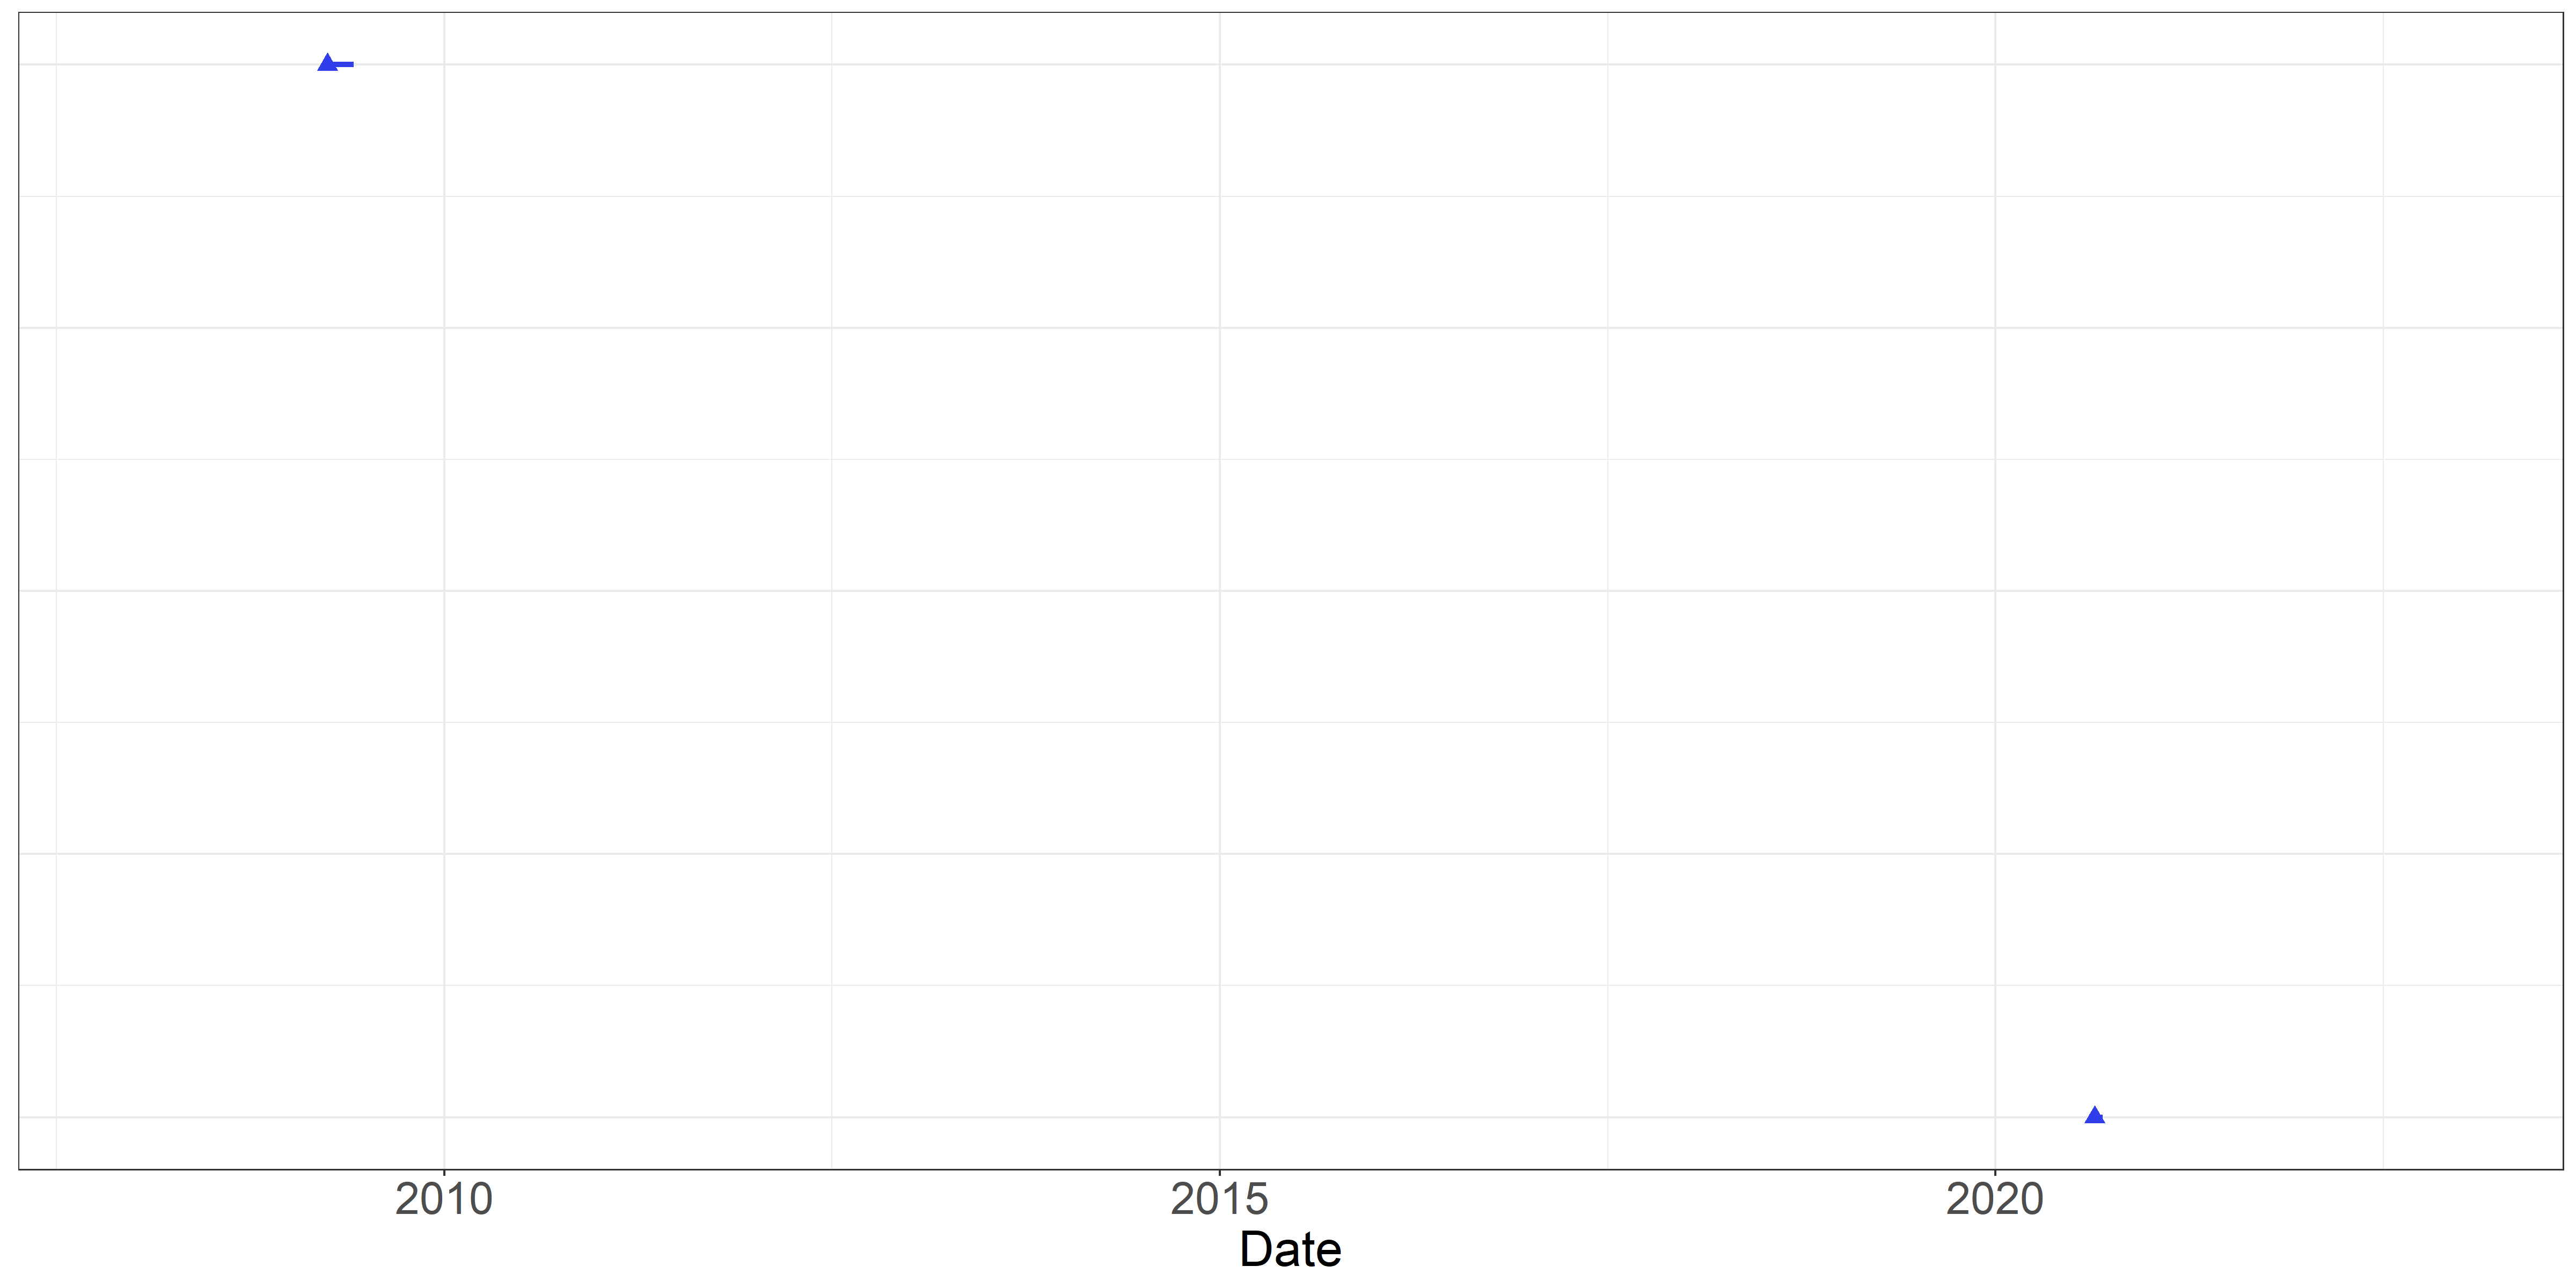
\includegraphics[width=1\linewidth]{../figures/SHIG_SSI_outbreaks} \caption{Placeholder caption}\label{fig:SHIGSSIoutbreaks}
\end{figure}

\subsection{Shiga toxin (verotoxin)-producing \textit{Escherichia coli}}

STEC primarily spreads through contaminated food. Less common sources of infection include contaminated drinking and bathing water, as well as direct or indirect contact with infected animals. Cattle and other ruminants are primary reservoirs for STEC serotypes that are frequently associated with human disease \autocite{Menge_2020}. Therefore, in Denmark, the source of infection is often products derived from beef, non-heat-treated dairy products, or other foods such as ready-to-eat vegetables, leafy greens, vegetable sprouts, and berries contaminated with feces from cows. \textit{Hemolytic uremic syndrome} (HUS) is a severe complication that, in some cases, particularly in children, can develop following an infection with STEC.



\begin{figure}[H]
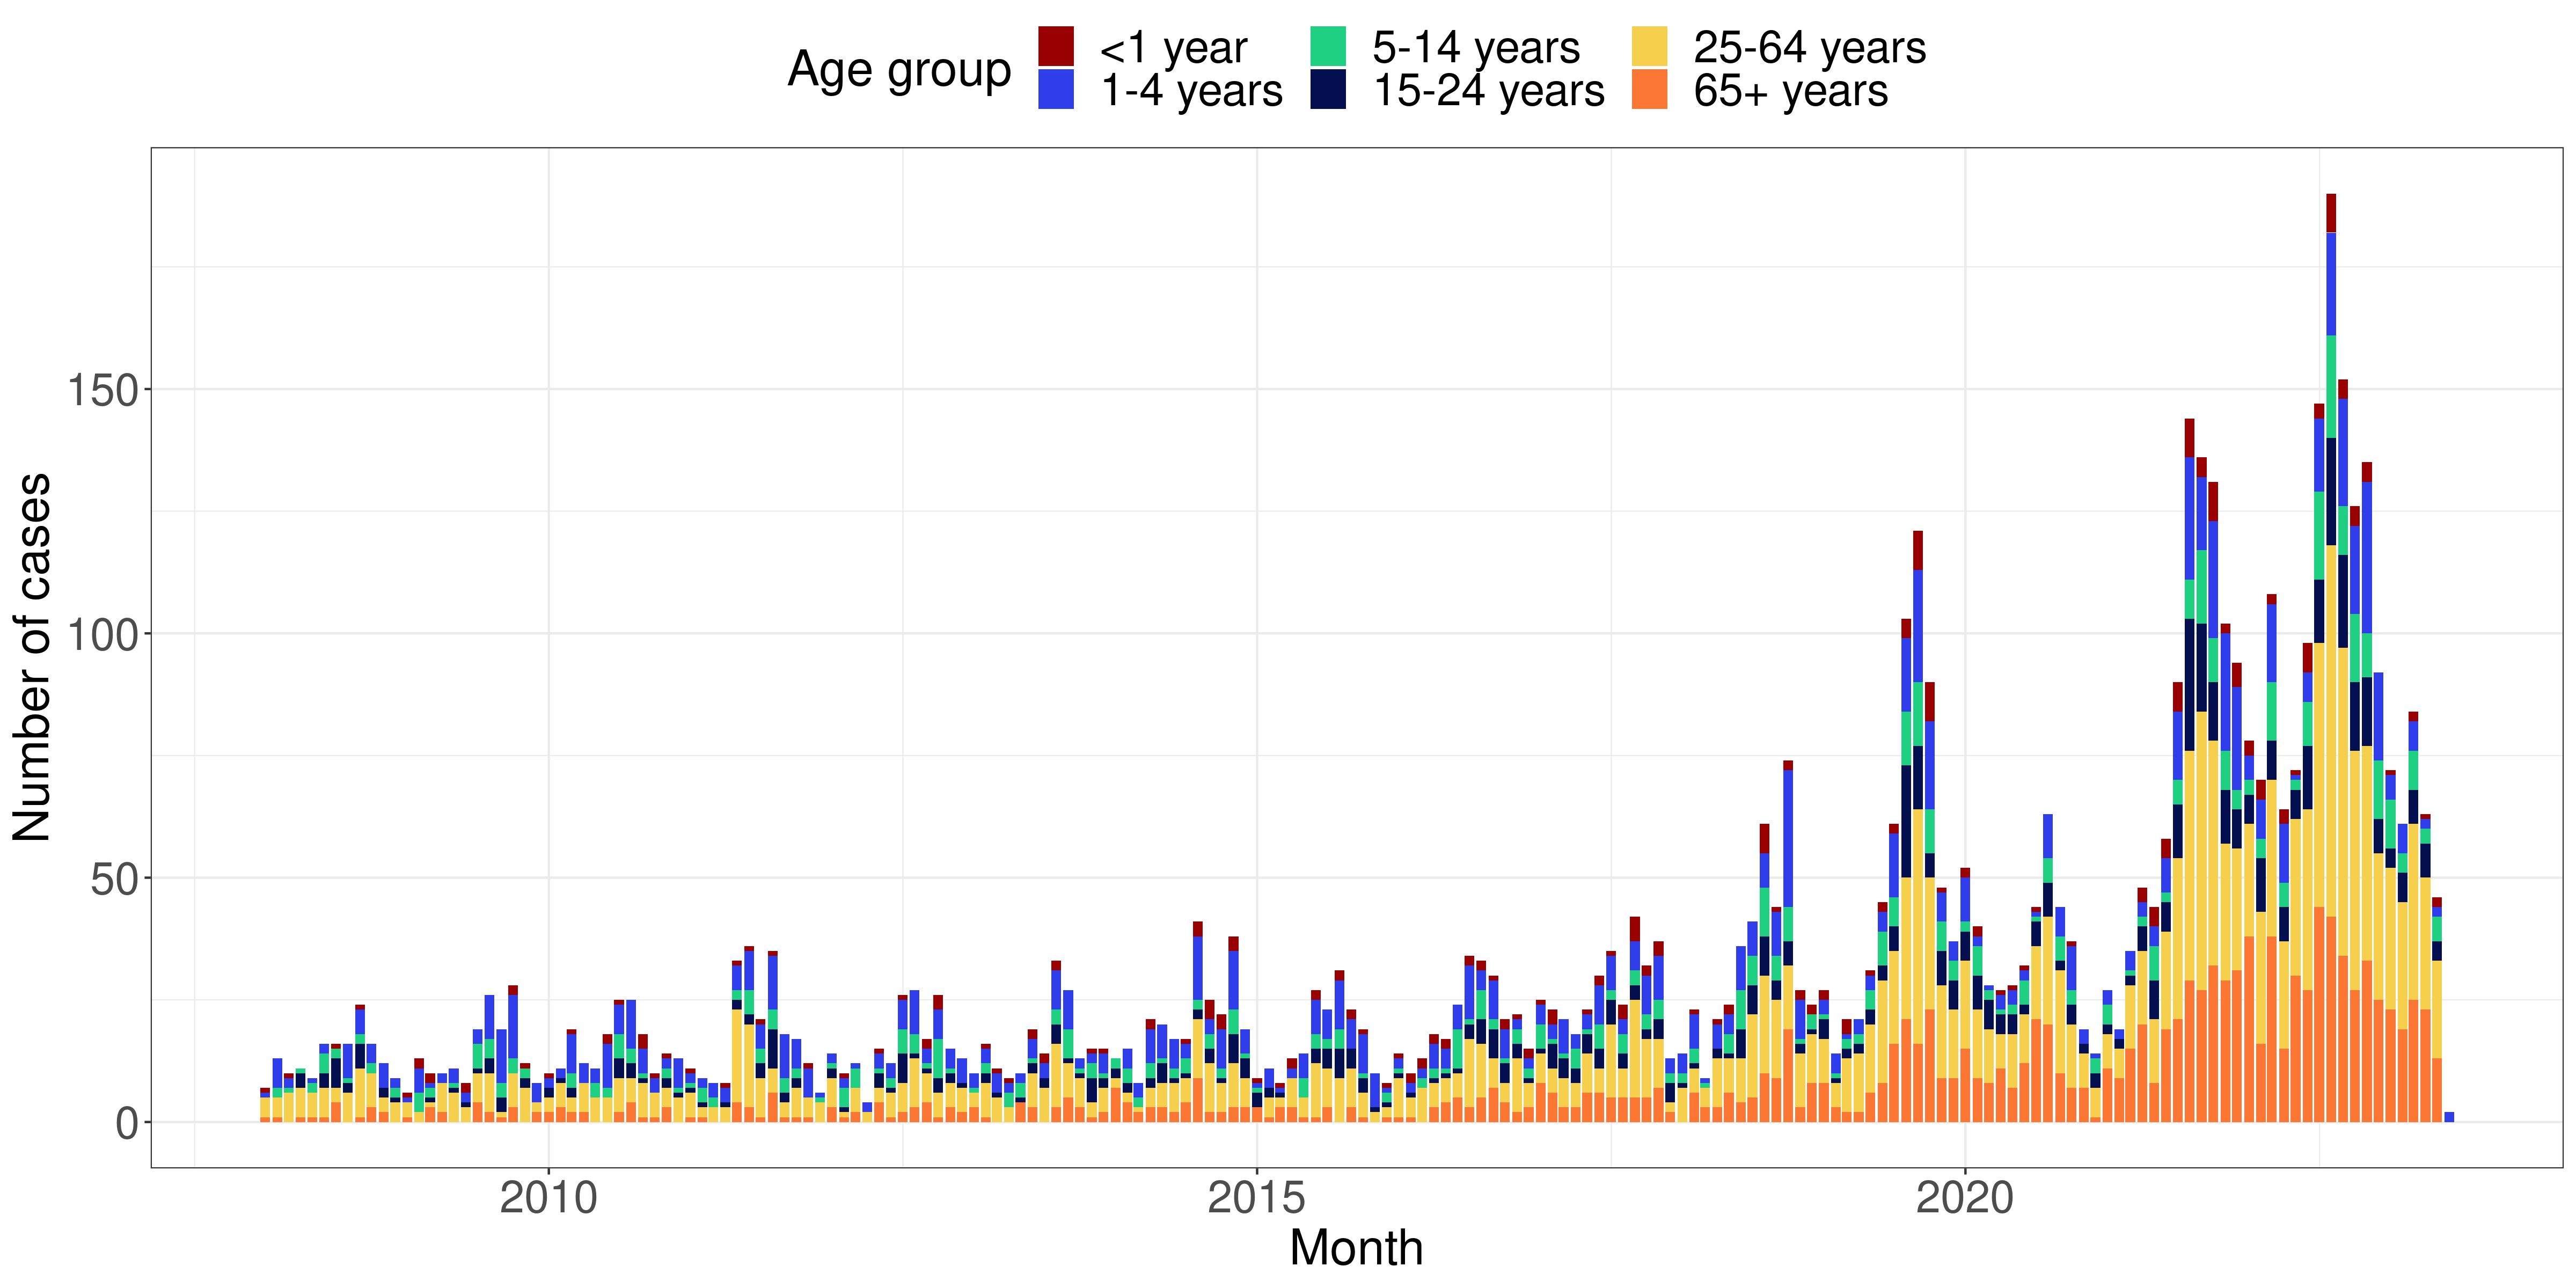
\includegraphics[width=1\linewidth]{../figures/STEC_long_plot} \caption{Placeholder caption}\label{fig:STECLongPlot}
\end{figure}

In general, stool samples are commonly used for diagnostic purposes in cases of STEC infections. Until 2018, most clinical microbiology departments relied on culture-based methods to detect and identify STEC bacteria in stool samples. However, in recent years, PCR methods have been increasingly adopted as a replacement for culture-based methods in the diagnosis of STEC infections \autocite{Svendsen_2023}. PCR methods offer advantages such as increased sensitivity and faster turnaround time, contributing to their growing popularity in clinical laboratories.

It is important to note that not all patients are routinely tested for STEC, and therefore, physicians need to specifically request STEC testing when submitting stool samples.

One of the earliest documented STEC outbreaks occurred in 2007, involving 18 laboratory-confirmed cases over a six-week period. The outbreak primarily affected children in daycare settings, and most patients experienced mild symptoms without bloody diarrhea. Investigations indicated a specific brand of organic beef sausage as the likely source of infection.

In September to October 2012, a STEC outbreak with a high risk of HUS was observed. Thirteen cases were diagnosed, with eight individuals developing HUS. Epidemiological investigations suggested that ground beef was the vehicle of the outbreak \autocite{Soborg_2013}.

More recent outbreaks include a 38-case outbreak from September to November 2018, with a suspected association with beef sausage as the source of infection. Additionally, there were two unresolved outbreaks with 11 and 14 cases occurring from May to July 2019 and from December 2021 to January 2022, respectively. The latter outbreak included three cases of HUS.



\begin{figure}[H]
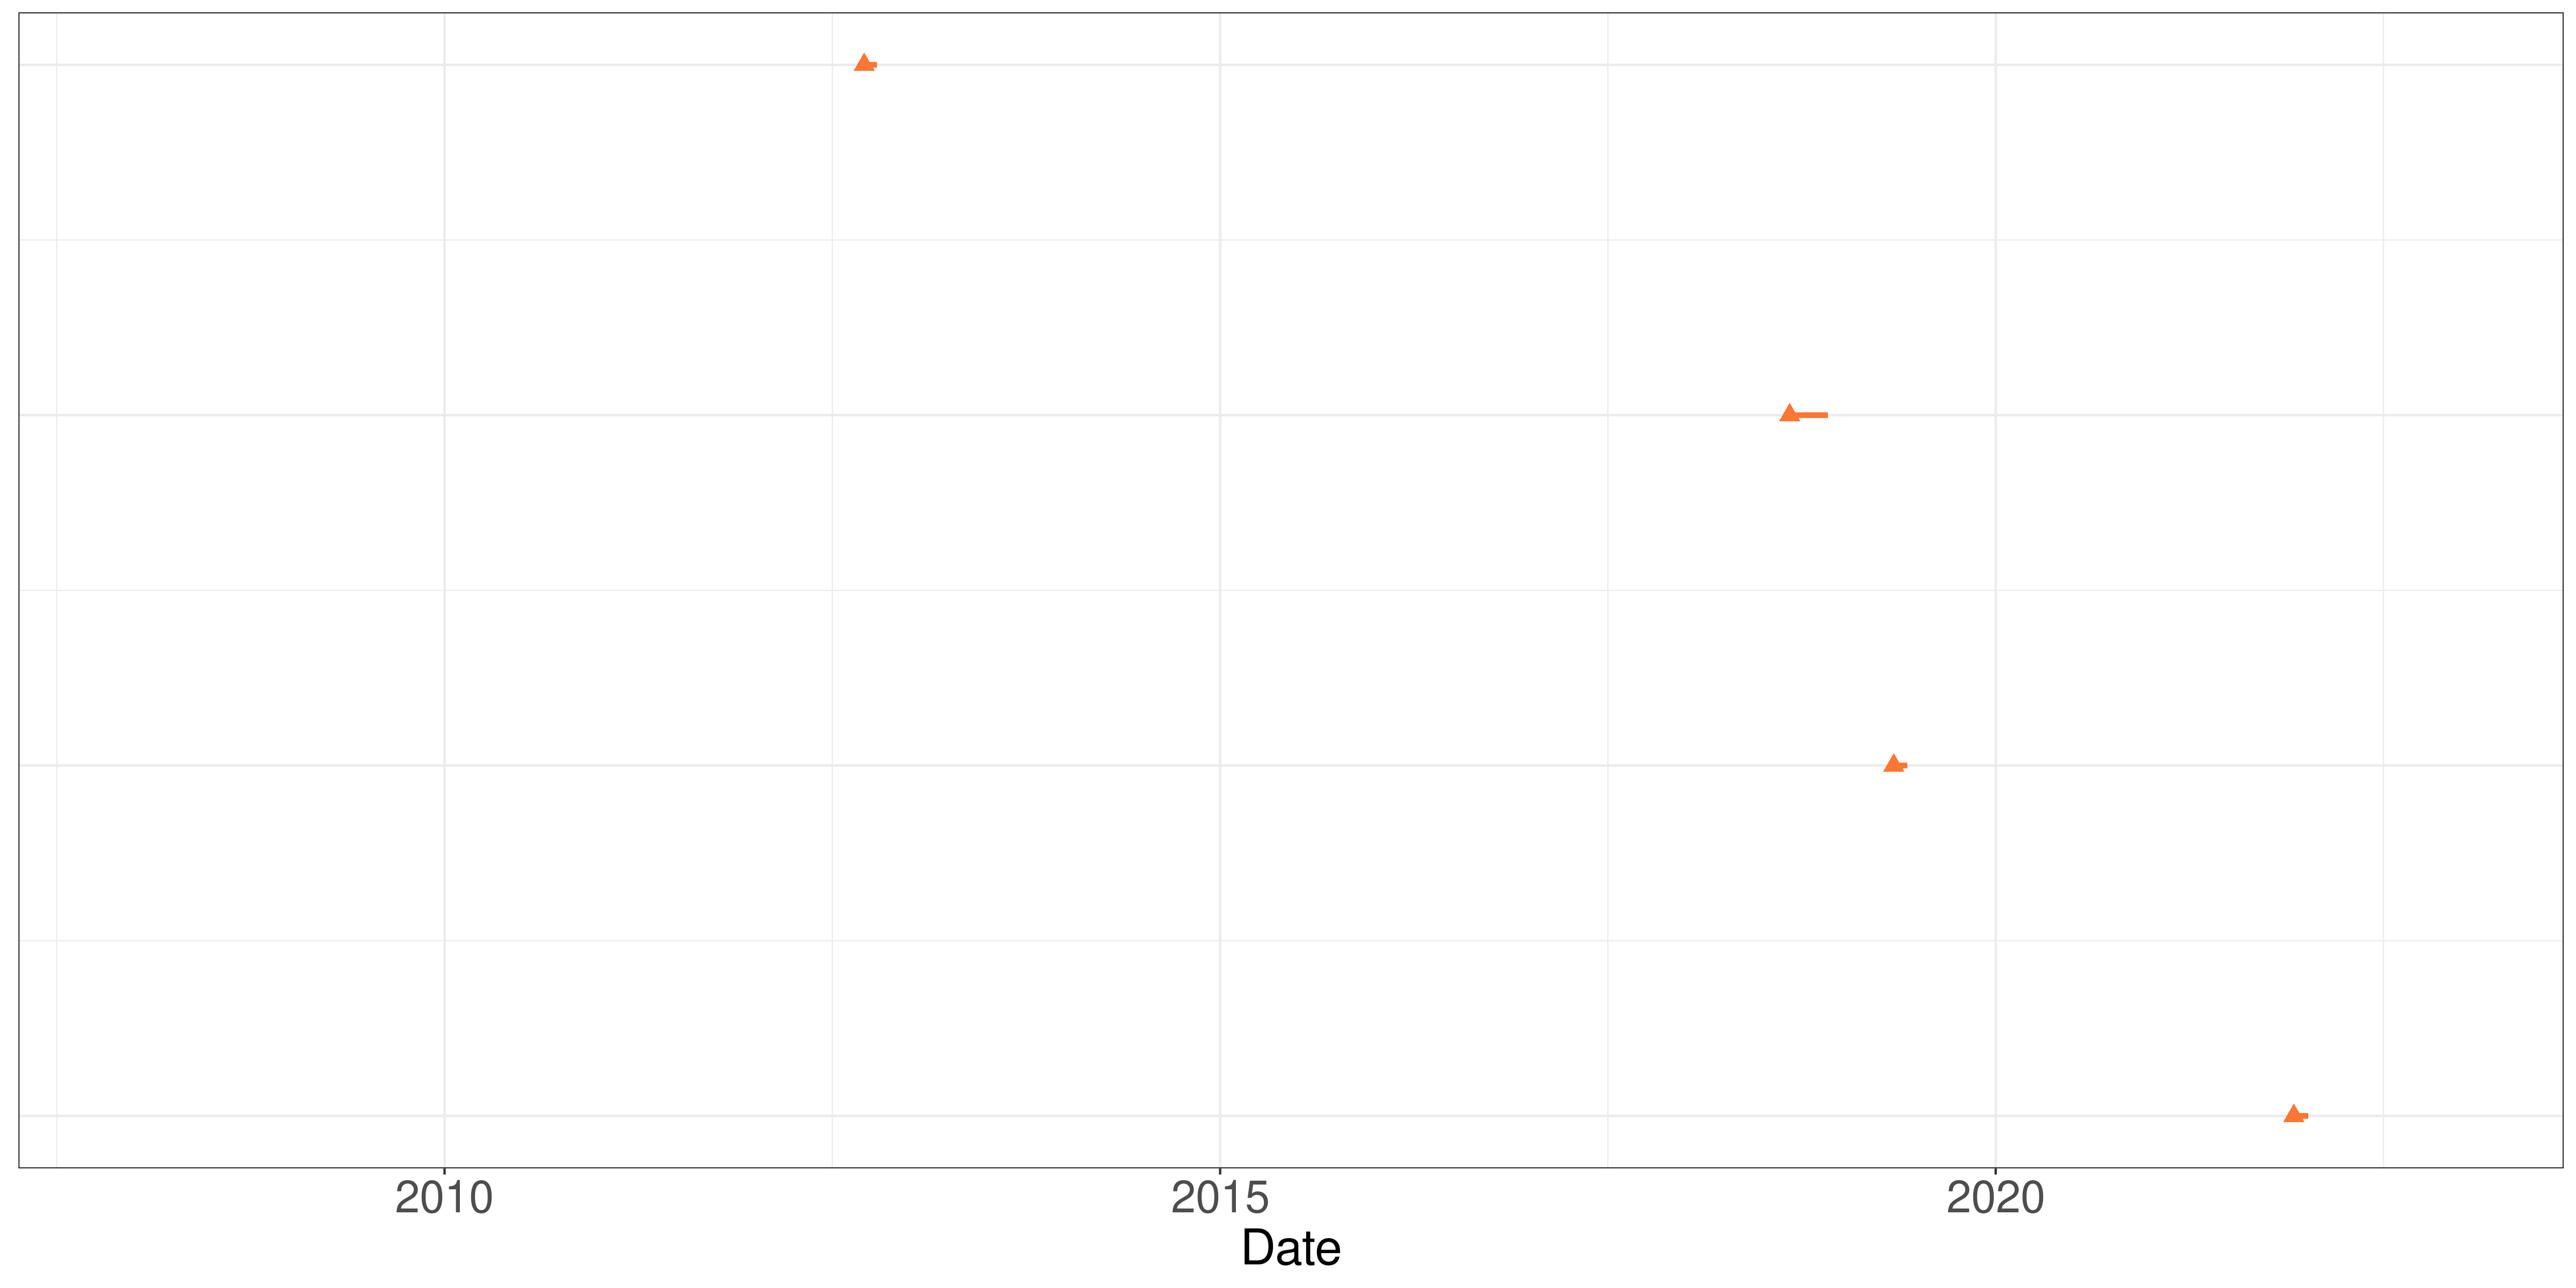
\includegraphics[width=1\linewidth]{../figures/STEC_SSI_outbreaks} \caption{Placeholder caption}\label{fig:STECSSIoutbreaks}
\end{figure}

\subsection{\textit{Salmonellosis}}

\textit{Salmonellosis} is a bacterial disease that primarily affects the intestinal tracts of humans. The \textit{Salmonella} bacteria are commonly found in the intestines of animals and humans and are excreted in feces. Human infection typically occurs through the consumption of contaminated food or water. Salmonella infections are often associated with the consumption of raw or undercooked meat, poultry, eggs or egg products, as well as unpasteurized milk.



\begin{figure}[H]
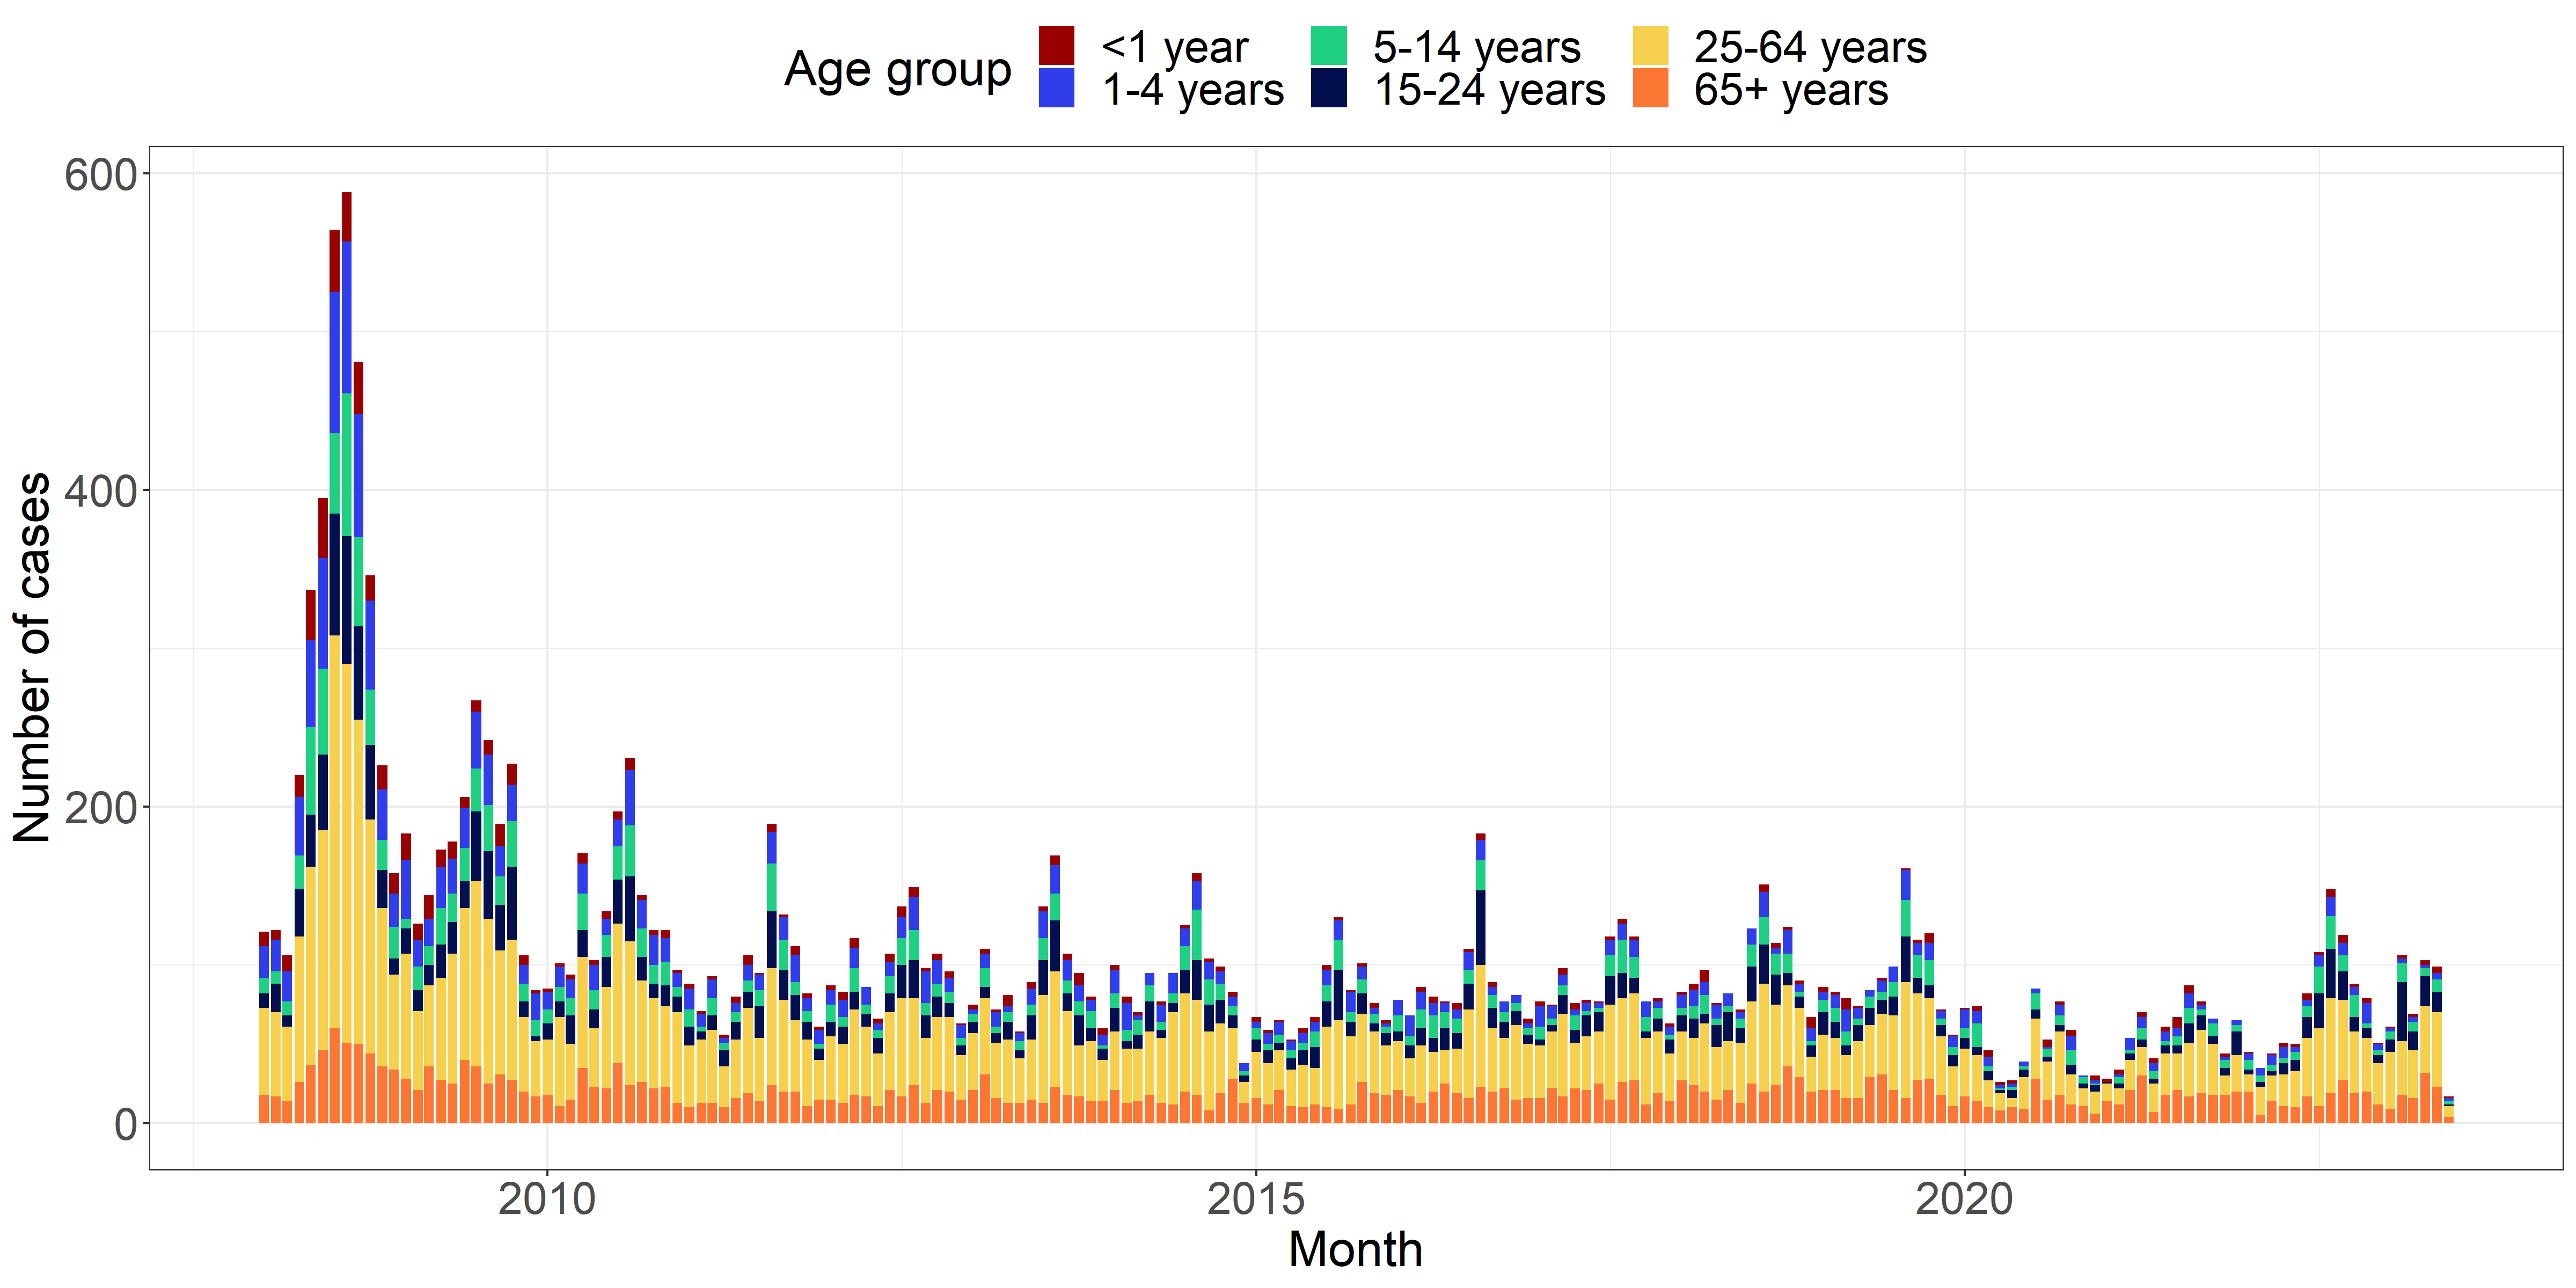
\includegraphics[width=1\linewidth]{../figures/SALM_long_plot} \caption{Placeholder caption}\label{fig:SALMLongPlot}
\end{figure}

It is worth noting that an increasing proportion of infections in Denmark are now observed in connection with international travel, particularly since \textit{Salmonella} has been eliminated from commercial chicken flocks in Denmark, making Danish eggs and poultry meat free from the bacteria. However, imported meat products can still pose a risk of contamination.

In 2015, three outbreaks of \textit{Salmonellosis} with patients in two or more regions were investigated \autocite{Helwigh_2016}:

\begin{itemize}
  \item An outbreak caused by \textit{S}. Newport affecting 6 people in the period from March to April 2015.
  \item A long-lasting outbreak caused by \textit{S}. Oranienburg with 14 genetically linked cases from July 2015 to January 2016.
  \item An outbreak with 6 patients from November 2015 to January 2016.
\end{itemize}

Other resolved and well-documented outbreaks include:

\begin{itemize}
  \item An outbreak with 49 cases from October 2018 to January 2019, where Mediterranean sausage was identified as a possible source of contamination.
  \item An outbreak with 45 cases from November 2020 to April 2021, linked to the consumption of the natural remedy HUSK Psyllium.
  \item An international outbreak from March to July 2021, with more than 300 cases in Europe, including 39 cases in Denmark. Imported melons were suspected as the source of infection.
  \item An outbreak caused by eggs from a Danish producer, resulting in 24 cases registered from September to November 2021.
  \item An international outbreak with a total of 392 cases across 12 countries in the EU/EEA and the UK, including 4 cases in Denmark. Kinder chocolate products were identified as the source of infection.
\end{itemize}

There were also outbreaks where it was not possible to identify the source of contamination, including:

\begin{itemize}
  \item An outbreak with 26 cases in the period from May to August 2019.
  \item An outbreak with 11 cases in the period from June to July 2020.
  \item An outbreak with 24 cases in the period from March to September 2022.
  \item An outbreak with 15 cases in the period from August to September 2022.
\end{itemize}



\begin{figure}[H]
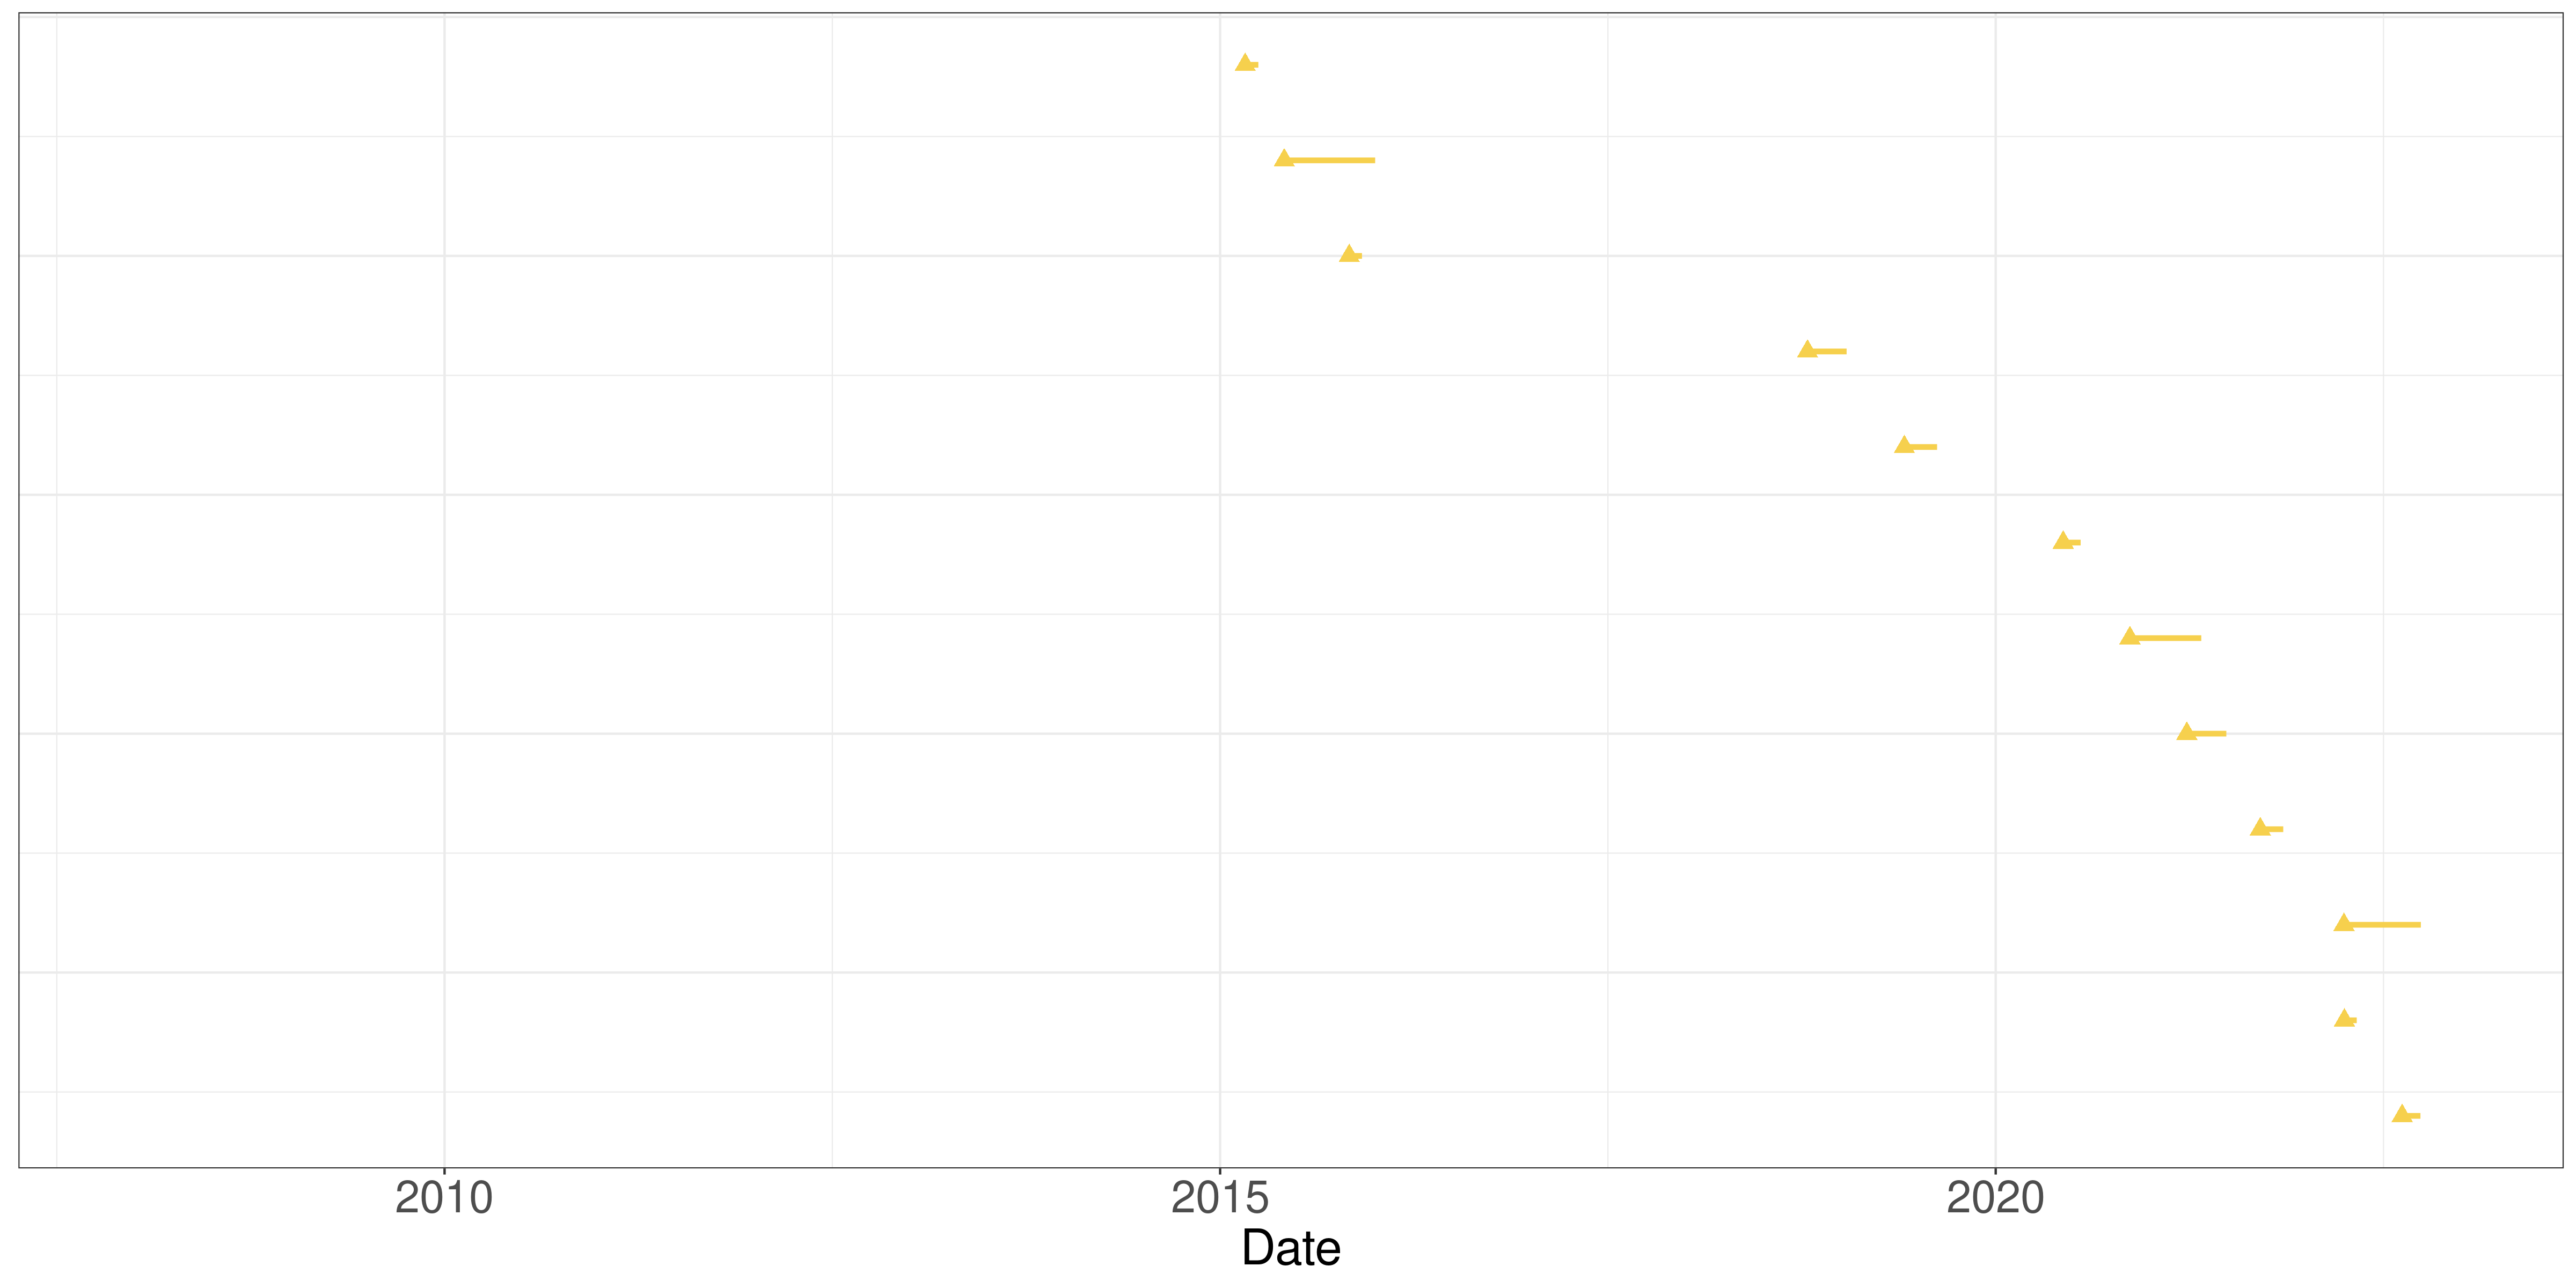
\includegraphics[width=1\linewidth]{../figures/SALM_SSI_outbreaks} \caption{Placeholder caption}\label{fig:SALMSSIoutbreaks}
\end{figure}

\cleardoublepage

\chapter{Methods}

In this chapter, the current state-of-the-art methods for disease outbreak detection will be outlined. Furthermore, the novel outbreak detection algorithm will be introduced, along with the theory related to generalized mixed effects models and hierarchical generalized linear models. These modeling frameworks are utilized in this master's thesis to analyze the count observations denoted as \(\boldsymbol{y}\), but more importantly they play a crucial role in assessing the unobserved random variables or random effects represented by \(\boldsymbol{u}\), which are directly employed in the detection algorithm for characterizing outbreaks.

Due to the complexity of generalized mixed effects models, obtaining closed-form solutions is generally not feasible. Therefore, an overview of the Laplace approximation technique will be provided in this chapter, which allows for approximating the likelihood function in these models. Additionally, the implementation of these models in the R programming language will be presented. The presentation of this chapter is mostly inspired by \textcite{Madsen_2010}.

\section{State-of-the-art outbreak detection algorithm}\label{StateOfTheArt}

In this section, the Farrington method introduced by \textcite{Farrington_1996} and the subsequent improvements proposed by \textcite{Noufaily_2013} will be outlined. These methods are recognized as the current state-of-the-art for disease outbreak detection and will be used as benchmarks to evaluate the performance of the novel outbreak detection algorithm proposed in this master's thesis. Both of the aforementioned methods have been implemented in the R package called \textbf{surveillance} by \textcite{Salmon_2016}, which can be accessed from the Comprehensive R Archive Network (CRAN) at \href{https://cran.r-project.org/web/packages/surveillance/index.html}{\nolinkurl{https://cran.r-project.org/web/packages/surveillance/index.html}}. The presentation of these methods are strongly inspired by \textcite{Salmon_2016}.

Both methods follow the same steps in the algorithm. The first step involves fitting an over-dispersed Poisson generalized linear model (GLM) with a log link to the reference data \(y_{t_{0}}\subseteq\{y_t;t\leq t_0\}\). In this model, the baseline count \(y_t\) corresponding to the baseline time point \(t\) is assumed to have an expected value \(\lambda_t\) and a variance \(\phi\lambda_t\), where \(\phi\geq1\) is ensured to account for over-dispersion. The systematic component of the model includes only a linear time trend in the frequency of reports. Therefore, the systematic component can be expressed as

\begin{equation}
  \log(\lambda_t)=\alpha+\beta t
\end{equation}

The original method incorporated seasonal effects by considering counts from comparable periods in past years for threshold calculation. This approach is similar to the one used by \textcite{Stroup_1989}. The baseline weeks, which are used as reference, are determined by two integers: \(b\) represents the number of years back, and \(w\) represents the window half-width. For a given current week \(x\) of year \(y\), only data from weeks \(x-w\) to \(x+w\) of years \(y-b\) to \(y-1\) are considered, resulting in a total of \(n=b(2w+1)\) baseline weeks. The default values are \(b=5\) and \(w=3\), resulting in a total of \(n=35\) baseline values.

However, \textcite{Noufaily_2013} demonstrated that the algorithm performs better when utilizing more historical data without disregarding seasonality. To achieve this, the author introduced a 10-level factor with a 7-week reference period and nine additional 5-week periods in each year. As a result, the systematic component of the model is modified as follows

\begin{equation}
\log(\lambda_t) = \alpha + \beta t + \delta_{j(t)}
\end{equation}

In this equation, \(j(t)\) represents the seasonal factor level corresponding to time point \(t\). The reference week \(t_0\) is always associated with the reference seasonal level, denoted by \(j(t_0) = 0\) and \(\delta_0 = 0\).

The idea of incorporating more data while preserving seasonality has been further expanded in the implementation of the method in the \textbf{surveillance} R package. The package allows the user to choose an arbitrary number of periods in each year. Consequently, the systematic component is adjusted as follows

\begin{equation}
\log(\lambda_t) = \alpha + \beta t + \delta_{c(t)}
\end{equation}

In this equation, \(c(t)\) represents the coefficients of a zero-order spline with \(\mathtt{noPeriods}+1\) knots. It can be conveniently represented as a \texttt{noPeriods}-level factor that captures seasonality. The function \(c(t)\) indicates which season or period of the year \(t\) belongs to.

Furthermore, \textcite{Noufaily_2013} demonstrated that it is beneficial to exclude the last 26 weeks before \(t_0\) from the baseline calculation. This exclusion helps prevent a reduction in sensitivity when an outbreak has recently started before \(t_0\).

In the second step, the algorithm predicts the expected number of counts \(\lambda_{t_0}\) for the current time point \(t_0\) using the fitted generalized linear model. Both methods differ in their assumptions for calculating the upper bound \(U_{t_0}\).

The original method assumes that a transformation of the prediction error, denoted as \(g(y_{t_0}-\hat{\lambda}_{t_0})\), follows a normal distribution. For example, when using the identity transformation \(g(x)=x\), the assumption becomes

\begin{equation}
y_{t_0} - \hat{\lambda}_{t_0} \sim \N(0, \V(y{t_0}-\hat{\lambda}_{t_0}))
\end{equation}

The upper bound of the prediction interval is then calculated based on this distribution. The variance of the prediction error is given by

\begin{equation}
\V(y_{t_0}-\hat{\lambda}_{t_0}) = \V(\hat{y}_{t_0}) + \V(\hat{\lambda}_{t_0}) = \phi\lambda_{t_0}
\end{equation}

Here, \(\V(\hat{y}_{t_0})\) represents the variance of an observation, and \(V(\hat{\lambda}_{t_0})\) represents the variance of the estimate. The threshold, defined as the upper bound of a one-sided \((1-\alpha)\cdot100\%\) prediction interval, is calculated as

\begin{equation}
U_{t_0} = \hat{\lambda}_{0} + z_{1-\alpha}\hat{V}(y_{t_0}-\hat{\lambda}_{t_0})
\end{equation}

However, this method's weakness lies in the assumption of normality itself. Therefore, an alternative assumption was presented in \textcite{Noufaily_2013}. This approach assumes that \(y_{t_0}\) follows a negative binomial distribution, denoted as \(\text{NB}(\lambda_{t_0}, \nu)\), where \(\lambda_{t_0}\) represents the mean and \(\nu = \frac{\lambda_{t_0}}{\phi-1}\) represents the over-dispersion parameter. In this parameterization, the expected value of \(y_t\) remains \(\lambda_t\), and the variance of \(y_t\) is \(\phi\lambda_t\), with \(\phi > 1\). If \(\phi \leq 1\), a Poisson distribution is assumed for the observed count. The threshold is defined as a quantile of the negative binomial distribution using the plug-in estimates \(\hat{\lambda}_{t_0}\) and \(\hat{\phi}\).

In the final step, the observed count \(y_{t_0}\) is compared to the upper bound \(U_{t_0}\), and an alarm is raised if \(y_{t_0} > U_{t_0}\). The fitting of the GLM in both methods involves three important steps.

First, the algorithm optionally performs a power transformation to correct for skewness and stabilize the variance of the data.

Next, the significance of the time trend is checked. The time trend is included in the model only if it is statistically significant at a chosen significance level, there are more than three years of reference data, and there is no over-extrapolation due to the time trend.

Finally, past outbreaks are reweighted based on their Anscombe residuals. If the Anscombe residual of a count exceeds a certain weight threshold, it is reweighted in a second fitting of the GLM. In the original method by \textcite{Farrington_1996}, a reweighting threshold of 1 was used. However, \textcite{Noufaily_2013} suggests using a value of 2.56 for the weight threshold to make the reweighting procedure less drastic, as it also reduces the variance of the observations.

\section{Novel outbreak detection algorithm}\label{Novel}

In this section, the novel algorithm for the prospective detection of disease outbreaks proposed in this master's thesis is outlined. The algorithm utilizes a generalized mixed effects model or a hierarchical generalized linear model as a modeling framework to model the count observations \(\boldsymbol y\) and assess the unobserved random effects \(\boldsymbol u\). These random effects are used directly in the detection algorithm to characterize an outbreak. The theoretical foundations of these models will be further discussed in Section \ref{GLMM} and Section \ref{HLMM}.

The first step involves fitting either a hierarchical Poisson Normal model or a hierarchical Poisson Gamma model with a log link to the reference data \(y_{t_0}\subseteq \{y_t;t\leq t_0\}\). Here, it is possible for the user to include an arbitrary number of covariates by supplying a model formula. In order to account for structural changes in the time series, e.g.~an improved and more sensitive diagnostic method or a new screening strategy at hospitals, a rolling window with width \(k\) is used to estimate the time-varying model parameters. Also, it is assumed that the count is proportional to the population size \(\boldsymbol n\). Hence, in terms of the canonical link the model for the fixed effects is

\begin{equation}
  \log(\lambda_{it})=x_{it}\beta+\log(n_{it}), \quad i=1,\dots,m, \quad t=T,\dots,0
\end{equation}

Here \(x_{it}\) and \(\beta\) are \(p\)-dimensional vectors of covariates and fixed effects parameters respectively, where \(p\) denotes the number of covariates or fixed effects parameters, \(m\) denotes the number of groups, and \(T\) denotes the length of the period, i.e.~\(T=t_0-k\).

In the second step, the algorithm infers the one-step ahead random effect \(u_{i{t}_1}\) for each group using the fitted model. The threshold for detecting outbreaks is defined as a quantile of the distribution of the random effects in the second stage model. This can be either a Gaussian distribution using the plug-in estimate \(\hat{\sigma}\) or a Gamma distribution using the plug-in estimate \(\hat{\phi}\).

In the final step, the inferred random effect \(u_{i{t}_1}\) is compared to the upper bound \(U_{t_0}\), and an alarm is raised if \(u_{i{t}_1}>U_{t_0}\). If an outbreak is detected, the related observation is omitted from the parameter estimation in the future. Thus, resulting in a smaller sample size for the rolling window until that specific observation is thrown away.

\section{General mixed effects models}\label{GLMM}

In this section selected theory related to generalized mixed effects models is presented. The general mixed effects model can be represented by its likelihood function

\begin{equation}\label{eq:glmm}
  L_{M}(\boldsymbol{\theta; y})=\int_{\mathbb{R}^{q}} L(\boldsymbol{\theta;u,y}) d\boldsymbol{u}
\end{equation}

where \(\boldsymbol{y}\) is the observed random variable, \(\boldsymbol{\theta}\) is the model parameters to be estimated and \(\boldsymbol{U}\) is the \(q\) unobserved random variables. The likelihood function \(L\) is the joint likelihood of both the observed and the unobserved random variables. The likelihood function for estimating \(\boldsymbol{\theta}\) is the marginal likelihood \(L_{M}\) obtained by integrating out the unobserved random variables. In general it is difficult to solve the integral in \eqref{eq:glmm} if the number of unobserved random variables is more than a few and hence numerical methods must be used. Thus, an outline of the Laplace approximation is included in this section.

\subsection{Hierarchical models}\label{hierarchicalModels}

It is useful to formulate the model as a hierarchical model containing a \textit{first stage model}

\begin{equation}
  f_{Y|u}(\boldsymbol{y;u,\beta})
\end{equation}

which is a model for the observed random variables given the unobserved random variables, and a \textit{second stage model}

\begin{equation}
  f_{U}(\boldsymbol{u; \Psi})
\end{equation}

which is a model for the unobserved random variables. Here \(\boldsymbol{\beta}\) represent the fixed effects parameters and \(\boldsymbol{\Psi}\) is a model parameter. The total set of parameters is \(\boldsymbol{\theta}=(\beta, \Psi)\). Hence the joint likelihood is given as

\begin{equation}
  L(\boldsymbol{\beta, \Psi; u, y})=f_{Y|u}(\boldsymbol{y;u,\beta}) f_{U}(\boldsymbol{u; \Psi})
\end{equation}

To obtain the likelihood for the model parameters \((\boldsymbol{\beta, \Psi})\) the unobserved random variables are integrated out. The likelihood function for estimating \((\boldsymbol{\beta, \Psi})\) is as in \eqref{eq:glmm} the marginal likelihood

\begin{equation}\label{eq:glmm2}
  L_{M}(\boldsymbol{\beta, \Psi; y})=\int_{\mathbb{R}^{q}} L(\boldsymbol{\beta, \Psi;u,y}) d\boldsymbol{u}
\end{equation}

where \(q\) is the number of unobserved random variables, and \(\boldsymbol{\beta}\) and \(\boldsymbol{\Psi}\) are the parameters to be estimated.

\subsection{Laplace Approximation}

The Laplace approximation will be outlined in the following. A thorough description of the Laplace approximation in nonlinear mixed effects models is found in \textcite{Wolfinger_1997}.

For a given set of model parameters \(\boldsymbol{\theta}\) the joint log-likelihood \(\ell(\boldsymbol{\theta, u, y})=\log\big(L(\boldsymbol{\theta, u, y})\big)\) is approximated using a second order Taylor approximation around the optimum \(\boldsymbol{\tilde{u}}=\boldsymbol{\hat{u}_\theta}\) of the log-likelihood function w.r.t. the unobserved random variables \(\boldsymbol{u}\), i.e.,

\begin{equation}\label{eq:laplaceApprox}
  \ell(\boldsymbol{\theta, u, y})\approx\ell(\boldsymbol{\theta, \tilde{u}, y}) - \frac{1}{2}(\boldsymbol{u-\tilde{u}})^T \boldsymbol{H}(\boldsymbol{\tilde{u}})(\boldsymbol{u-\tilde{u}})
\end{equation}

where the first-order term of the Taylor expansion disappears since the expansion is done around the optimum \(\boldsymbol{\tilde {u}}\) and \(\boldsymbol{H}(\boldsymbol{\tilde{u}})=-\ell_{uu}''(\boldsymbol{\theta, u, y})|_{\boldsymbol{u=\tilde{u}}}\) is the negative Hessian of the joint log-likelihood evaluated at \(\boldsymbol{\tilde{u}}\).

It is readily seen that the joint log-likelihood for the hierarchical model specified in Section \ref{hierarchicalModels} is

\begin{equation}
  \ell(\boldsymbol{\theta, u, y}) = \ell(\boldsymbol{\beta, \Psi, u, y}) = \log f_{Y|u}(\boldsymbol{y;u,\beta})+\log f_U(\boldsymbol{u;\Psi})
\end{equation}

which implies that the Laplace approximation becomes

\begin{equation}
  \ell_{M,LA}(\boldsymbol{\theta, y})=\log f_{Y|u}(\boldsymbol{y; \tilde{u},\beta})+\log f_U(\boldsymbol{\tilde{u}, \Psi})-\frac{1}{2}\log\Bigg|\frac{\boldsymbol{H}(\boldsymbol{\tilde{u}})}{2\pi}\Bigg|
\end{equation}

\subsection{Formulation of the hierarchical model}

\begin{theorem}[Hierarchical Poisson Normal model]
\protect\hypertarget{thm:poisnTheorem}{}\label{thm:poisnTheorem}In order to simplify the notation, the probability density functions are presented for a specific observation and hence the subscripts indicating the group and time are omitted. The conditional distribution of the count observations is assumed to be a Poisson distribution with intensities \(\boldsymbol \lambda\)

\begin{equation}
  f_{Y|u}(y; u, \boldsymbol{\beta})=\frac{\lambda\exp(u)^{y}}{y!}\exp\big(-\lambda\exp(u)\big)
\end{equation}

Also, it is assumed that the count is proportional to the population size \(\boldsymbol{x}\). Hence, in terms of the canonical link for the Poisson distribution the model for the fixed effects is

\begin{equation}
  \log(\lambda_{it})=\boldsymbol{X}_{t}^T\boldsymbol{\beta}+\log(x_{it}), \quad i=1,\dots,m, \quad t=1,\dots,T
\end{equation}

The probability density function for the distribution of the random effects is assumed to follow a Gaussian distribution, \(\boldsymbol u\sim\N(\boldsymbol 0,sigma^2)\), i.e.

\begin{equation}
  f_U(u;\sigma)=\frac{1}{\sigma\sqrt{2\pi}}\exp\Bigg(-\frac{u^2}{2\sigma^2}\Bigg)
\end{equation}

where \(\sigma\) is a model parameter.

Henceforth, the total set of parameters are \(\boldsymbol{\theta}=(\boldsymbol{\beta},\sigma)\) and the model can be formulated as a two-level hierarchical model

\begin{subequations} \label{eq:PoisN}
  \begin{alignat}{2}
    \boldsymbol{Y|u} &\sim \Pois \big( \boldsymbol{\lambda} \exp(\boldsymbol{u}) \big) \label{eq:pois_n0} \\ 
    \boldsymbol{u} &\sim \N(\boldsymbol{0},I\sigma^2) \label{eq:pois_n1}
  \end{alignat}
\end{subequations}

The joint likelihood for the count observations \(\boldsymbol y\) and the random effects \(\boldsymbol u\) becomes

\begin{multline}\label{eq:jnllPoisN}
  L(\boldsymbol{\beta}, \sigma;u_{it},y_{it})=\\
  \prod_{t=1}^{T}\prod_{i=1}^{m} \frac{(\lambda_{it}\exp(u_{it}))^{y_{it}}}{y_{it}!}\exp\big(-\lambda_{it}\exp(u_{it})\big) \prod_{t=1}^{T}\prod_{i=1}^{m} \frac{1}{\sigma\sqrt{2\pi}}\exp\Bigg(-\frac{u_{it}^2}{2\sigma^2}\Bigg)
\end{multline}
\end{theorem}

\section{Hierarchical generalized linear models}\label{HLMM}

In this section selected theory related to hierarchical generalized linear models is presented. The model class was initially formulated by \textcite{Lee_1996} as a natural generalization of the generalized linear models to also incorporate random effects. A starting point in hierarchical modelling is an assumption that the distribution of random effects may be modeled by an exponential dispersion family. This family of models were first introduced by \textcite{Fisher_1922}, and has proven to play an important role in mathematical statistics because of their simple inferential properties. The exponential dispersion family considers a family of distributions, which can be written on the form

\begin{equation}\label{eq:expDispFam}
  f_Y(y;\theta)=c(y,\lambda)\exp\big(\lambda \{\theta y-\kappa(\theta) \}\big)
\end{equation}

Here the parameter \(\lambda>0\) is called the \textit{precision parameter}, which in some cases represents a known shape parameter as for the Gamma distribution. In other cases the precision parameter represents an over-dispersion that is not related to the mean. These distributions combine with the so-called \textit{standard conjugate distributions} in a simple way, and lead to marginal distributions that may be expressed in a closed form suited for likelihood calculations.

\subsection{Standard conjugate distribution}

Now the general notion of a \textit{standard conjugate distribution} for an exponential dispersion family is introduced.

Consider an exponential dispersion family \(\ED(\mu, \V(\mu)/\lambda)\) with density \eqref{eq:expDispFam} for \(\theta\in\Omega\). Let \(\mathcal{M}=\tau(\Omega)\) denote the mean value space for this family. Let \(m\in\mathcal{M}\) and consider

\begin{equation}\label{eq:densityTheta}
  g_{\theta}(\theta;m, \gamma)=\frac{1}{C(m,\gamma)}\exp\Big(\frac{\theta m-\kappa(\theta)}{\gamma}\Big)
\end{equation}

with

\begin{equation}
  C(m,\gamma)=\int_\Omega \exp\Big(\frac{\theta m-\kappa(\theta)}{\gamma}\Big)d\theta
\end{equation}

for \(\gamma\in\mathbb{R}_+\) for which the integral converges. Then \eqref{eq:densityTheta} defines the density function of a probability distribution for \(\theta\). This distribution is called the \textit{standard conjugate distribution} for \(\theta\) corresponding to \eqref{eq:expDispFam}.

\subsection{Definition of the hierarchical generalized linear model}

Consider a set of observations \(\boldsymbol Y=(Y_1,Y_2,\dots,Y_k)^T\) such that for a given value of a parameter \(\theta\) the distribution of \(Y_i\) is given by an exponential dispersion model with density \eqref{eq:expDispFam} and with canonical parameter space \(\Omega\) (for \(\theta\)), mean value \(\mu=\kappa'(\theta)\), mean value space \(\mathcal{M}\) (for \(\mu\)) and canonical link \(\theta=g(\mu)\).

Let the \textit{conjugate distribution} of \(\theta\) be given by \eqref{eq:densityTheta}, and the corresponding conjugate distribution of \(\mu\), (e.g., \(f_Y(y)\) Poisson distribution; \(g_\mu(\mu)\) Gamma distribution; link \(g(\mu)=\log(\mu)\)).

The variables in a hierarchical generalized linear model are

\begin{enumerate}[i)]
  \item the observed responses $y_1, y_2, \dots, y_k \quad (\in\mathcal{M})$
  \item the unobserved random effects $u_1,u_2,\dots,u_q \quad (\in\mathcal{M})$
  \item and the corresponding unobserved canonical variables $v_i=g(u_i) \quad (\in \Omega)$
\end{enumerate}

The \textit{linear predictor} is of the form

\begin{equation}
  \boldsymbol \theta = g(\boldsymbol \mu|\boldsymbol v)=\boldsymbol{X\beta}+\boldsymbol{Zv}
\end{equation}

The distribution of \(\boldsymbol V\in\Omega\) is a conjugated distribution to the canonical parameter \(\theta\). The derived distribution of \(\boldsymbol U\in\mathcal{M}\) is the corresponding conjugated distribution to the mean value parameter \(\mu\) such that \(\E[U]=\psi\). When the conditional distribution of \(Y|\mu\) is a Poisson distribution, and the distribution of \(V\) is constructed in such a way that the distribution of \(U=\log(V)\) is a Gamma distribution with mean value \(\E[U]=\psi=1\), then it follows that the distribution of \(Y\) is a negative binomial distribution with parameters determined by \(\boldsymbol{X\beta}\) and \(\boldsymbol{Zv}\).

\subsection{Formulation of the hierarchical Poisson Gamma model}

To motivate the choice of distribution for unobserved random variables \(\boldsymbol U\), an illustrative example is presented.

INCLUDE AN EXAMPLE

\begin{verbatim}
## # A tibble: 2 x 3
##   ageGroup  `mean(y)` `var(y)`
##   <fct>         <dbl>    <dbl>
## 1 <65 years      1.21     1.57
## 2 65+ years      3.23     5.58
\end{verbatim}

\begin{theorem}[Compound Poisson Gamma model]
\protect\hypertarget{thm:poisgTheorem}{}\label{thm:poisgTheorem}In the compound Poisson Gamma model the conditional distribution of the count observations are assumed to be a Poisson distribution with intensities \(\boldsymbol \lambda\)

\begin{equation}\label{eq:pdfPois}
  f_{Y|u}(y;u,\boldsymbol{\beta})=\frac{(\lambda u)^{y}}{y!}\exp(-\lambda u)
\end{equation}

The probability density function for the random effects \(\boldsymbol u\) are assumed to follow a reparametrized Gamma distribution with mean \(\boldsymbol 1\), \(\boldsymbol u \sim \G(\boldsymbol 1/\phi,\phi)\) that is

\begin{equation} \label{eq:pdfGamma}
  f_{u}(u;\phi)=\frac{1}{\phi \Gamma(1/\phi)} \bigg(\frac{u}{\phi}\bigg)^{1/\phi-1} \exp (-u/\phi)
\end{equation}

Subsequently, the model can be formulated as a two-level hierarchical model

\begin{subequations} \label{eq:PoisGam}
  \begin{alignat}{2}
    \boldsymbol{Y|u} &\sim \Pois (\boldsymbol{\lambda u}) \label{eq:pois_g0} \\ 
    \boldsymbol{u} &\sim \G(\boldsymbol 1/\phi,\phi) \label{eq:pois_g1}
  \end{alignat}
\end{subequations}

Given \eqref{eq:pdfPois} and \eqref{eq:pdfGamma}, the probability function for the marginal distribution of \(\boldsymbol Y\) is determined from

\begin{equation} \label{eq:marMix}
  \begin{aligned}
    g_{Y}(y;\boldsymbol \beta,\phi)&=\int_{u=0}^\infty f_{Y|u}(y;\boldsymbol, u, \beta) f_{u}(u;\phi) \,du \\
    &=\int_{u=0}^\infty \frac{(\lambda u)^y}{y!} \exp (-\lambda u) \frac{1}{\phi \Gamma(1/\phi)} \bigg(\frac{u}{\phi}\bigg)^{1/\phi-1} \exp (-u /\phi) \,du\\
    &=\frac{\lambda^{y}}{y!\Gamma(1/\phi)\phi^{1/\phi}} \int_{u=0}^\infty u^{y+1/\phi-1} \exp \big(-u(\lambda \phi+1)/\phi\big) \,du
  \end{aligned}
\end{equation}

In \eqref{eq:marMix} it is noted that the integrand is the \emph{kernel} in the probability density function for a Gamma distribution, \(\G\big(y+1/\phi,\phi/(\lambda \phi+1)\big)\). As the integral of the density shall equal one, we find by adjusting the norming constant that

\begin{equation}
  \int_{u=0}^\infty  u^{ y+ 1/\phi-1} \exp \bigg(- u/\Big(\phi/( \lambda \phi+1)\Big)\bigg) \,du = \frac{\phi^{ y+ 1/\phi}\Gamma( y+\boldsymbol 1/\phi)}{( \lambda \phi + 1)^{y+1/\phi}}
\end{equation}

Therefore, it can be shown that the marginal distribution of \(Y\) is a negative binomial distribution, \(Y\sim\NB\big(1/\phi,1/(\lambda\phi+1)\big)\). The probability function for \(Y\) is

\begin{equation} \label{eq:pdfMix}
  \begin{aligned}
    P[Y=y]&=g_{Y}(y;\boldsymbol \beta, \phi) \\
    &=\frac{\lambda^{y}}{y!\Gamma(1/\phi)\phi^{1/\phi}}\frac{\phi^{y+1/\phi}\Gamma(y+1/\phi)}{(\lambda \phi + 1)^{y+1/\phi}} \\
    &=\frac{\Gamma(y+1/\phi)}{\Gamma(1/\phi)y!}\frac{1}{(\lambda\phi+1)^{1/\phi}}\bigg(\frac{\lambda\phi}{\lambda\phi+1}\bigg)^{y} \\
    &=\begin{pmatrix} y+1/\phi-1 \\ y \end{pmatrix} \frac{1}{(\lambda\phi+1)^{1/\phi}}\bigg(\frac{\lambda\phi}{\lambda\phi+1}\bigg)^{y} \ , \quad \mathrm{for} \ y = 0, 1, 2, \dots
  \end{aligned}
\end{equation}

where we have used the convention

\begin{equation}
  \begin{pmatrix} z\\y \end{pmatrix} = \frac{\Gamma(z+1)}{\Gamma(z+1-y)y!}
\end{equation}

for \(z\) real and \(y\) integer values. Consequently, the mean and variance of \(Y\) are given by

\begin{equation}
  \E[Y] = \lambda \qquad \V[Y] = \lambda (\lambda \phi + 1)
\end{equation}

The likelihood function for estimating \((\boldsymbol \beta,\phi)\) is

\begin{equation}
  L(\boldsymbol \beta, \phi; y_{it})=\prod_{t=1}^{T}\prod_{i=1}^{m} \begin{pmatrix} y_{it}+1/\phi-1 \\ y_{it} \end{pmatrix} \frac{1}{(\lambda_{it}\phi+1)^{1/\phi}}\bigg(\frac{\lambda_{it}\phi}{\lambda_{it}\phi+1}\bigg)^{y_{it}}
\end{equation}
\end{theorem}

\subsubsection{Inference on individual groups}

In order to simplify the notation, the subscript indicating the group and time are omitted. Consider the compound Poisson Gamma model in \eqref{eq:PoisGam}, and assume that a value \(Y=y\) has been observed.

Then the conditional distribution of \(u\) for given \(Y=y\) is found using Bayes Theorem

\begin{equation}
  \begin{aligned}
    g_{u}(u|Y=y)&=\frac{f_{y,u}(y,u)}{g_Y(y;\lambda, \phi)} \\
    &=\frac{f_{y|u}(y;u)g_{u}(u)}{g_{Y}(y;\lambda,\phi)} \\
    &=\frac{1}{g_{Y}(y;\lambda,\phi)}\bigg(\frac{(\lambda u)^y}{y!} \exp (-\lambda u) \frac{1}{\phi \Gamma(1/\phi)} \bigg(\frac{u}{\phi}\bigg)^{1/\phi-1} \exp (-u/\phi)\bigg) \\
    &\propto u^{y+1/\phi-1} \exp \big(- u(\lambda\phi+1)/\phi\big)
  \end{aligned}
\end{equation}

We identify the \emph{kernel} of the probability density function

\begin{equation}
  u^{y+1/\phi-1} \exp (- u(\lambda\phi+1)/\phi)
\end{equation}

as the kernel of a Gamma distribution, \(\G(y+1/\phi,\phi/(\lambda\phi+1))\), i.e.~the conditional distribution of \(u\) for given \(Y=y\) can be written as

\begin{equation}
  u| Y=y\sim \G\big(y+1/\phi,\phi/(\lambda \phi+1)\big)
\end{equation}

The mean of the conditional distribution is given by:

\begin{equation}
  \E[u|Y=y]=\frac{y\phi+1}{\lambda \phi+1}
\end{equation}

And the variance of the conditional distribution is:\\
\begin{equation}
  \V[u|Y=y]=\frac{( \phi^2+\phi)}{(\lambda \phi + 1)^2}
\end{equation}

These formulas provide the mean and variance of the conditional distribution of \(u\) given the observed value \(Y=y\).

\subsubsection{Why do we choose the Gamma distribution to represent the variation between days?}

The choice of the Gamma distribution for modeling the random effects has been motivated by several reasons. Firstly, the support of the Gamma distribution, which ranges from 0 to infinity, aligns with the mean-value space, denoted as \(\mathcal{M}\), for the Poisson distribution. This ensures that the random effects are constrained within a meaningful range for the underlying Poisson process.

Secondly, the two-parameter family of Gamma distributions offers considerable flexibility, encompassing a wide range of shapes and distributions that can span from exponential-like distributions to fairly symmetrical distributions on the positive real line. This flexibility allows the model to capture various patterns and characteristics observed in the data.

Additionally, the choice of the Gamma distribution has benefits in terms of the derivation of the marginal distribution of the response variable \(Y\). The kernel \(u^{\alpha-1}\exp(-u/\beta)\) of the Gamma distribution used for modeling the random effects exhibits a similar structure to the kernel \(u^y\exp(-u)\) of the likelihood function corresponding to the sampling distribution of \(Y\). This similarity facilitates the analytical computation of the integral involved in deriving the marginal distribution, as it can be expressed in terms of known functions.

Overall, the Gamma distribution is selected due to its alignment with the mean-value space of the Poisson distribution, its flexibility in capturing diverse distributions, and its analytical convenience in computing the marginal distribution of the response variable.

\section{Parameter estimation}

In this section, the parameter estimation and implementation of the novel outbreak detection algorithm in R using the \textbf{TMB} (Template model Builder) package is presented. \textbf{TMB} is an open-source R package developed by \textcite{Kristensen_2016}. This package facilitates efficient maximum likelihood estimation and uncertainty calculations for the parameter set \(\boldsymbol \theta=(\boldsymbol{\beta, \Psi})\) and random effects \(\boldsymbol u\). The presentation of the parameter estimation conducted in \textbf{TMB} is strongly inspired by Chapter 2 in \textcite{Kristensen_2016} and Section 5.10 in \textcite{Madsen_2010}.

The \textbf{TMB} package maximizes a user-provided objective function in the form of a C++ template to estimate the maximum likelihood for the parameter set \(\boldsymbol \theta = (\boldsymbol{\beta, \Psi})\). See Appendix \ref{cpp} to access the C++ template files used in this master's thesis. The objective function maximizes the marginal log-likelihood function, which integrates out the random effects \(\boldsymbol u\)

\begin{equation}
  \ell_{M}(\boldsymbol{\theta; y})=\int_{\mathbb{R}^{q}} \ell (\boldsymbol{\theta;u,y}) d\boldsymbol{u}
\end{equation}

where \(\ell(\boldsymbol{\theta, u,y})\) is the joint log-likelihood function of the data given the parameters and random effects. We use \(\hat{\boldsymbol u}_{\boldsymbol \theta}\) to denote the maximizer of the joint log-likelihood \(\ell(\boldsymbol{\theta;u,y})\) w.r.t. \(\boldsymbol u\); i.e.,

\begin{equation}
  \hat{\boldsymbol u}_{\boldsymbol \theta}=\argmax_{\boldsymbol u} \ell(\boldsymbol{\theta;u,y})
\end{equation}

Using \(H(\hat{\boldsymbol u}_{\boldsymbol \theta})\) to denote the negative Hessian of the joint log-likelihood evaluated at \(\hat{\boldsymbol u}_{\boldsymbol \theta}\); i.e,

\begin{equation}
  H(\hat{\boldsymbol u}_{\boldsymbol \theta}) =-\ell_{uu}''(\boldsymbol{\theta, u, y})|_{\boldsymbol u=\hat{\boldsymbol u}_{\boldsymbol \theta}}
\end{equation}

The Laplace approximation for the marginal log-likelihood \(\ell_M(\boldsymbol \theta)\) is

\begin{equation}
  \ell_{M,LA}(\boldsymbol{\theta, y})=\ell(\boldsymbol{\theta,u,y})-\frac{1}{2}\log \Big|\frac{H(\hat{\boldsymbol u}_{\boldsymbol \theta})}{2\pi}\Big|
\end{equation}

Our estimate of \(\theta\) minimizes the negative log of the Laplace approximation, i.e.,

\begin{equation}
  -\ell_{M,LA}(\boldsymbol{\theta, y}) = - \ell(\boldsymbol{\theta, u, y}) + \frac{1}{2} \log \Big|\frac{H(\hat{\boldsymbol u}_{\boldsymbol \theta})}{2\pi} \Big|
\end{equation}

The maximization of the Laplace approximation for the marginal likelihood is then performed using conventional R optimization routines (e.g., BFGS) to optimize the objective and obtain our estimate \(\hat{\boldsymbol \theta}\). Uncertainty of the estimate \(\hat{\boldsymbol \theta}\), or any differentiable function of the estimate \(\phi(\hat{\boldsymbol \theta})\), is obtained by the \(\delta\)-method:

\begin{equation}
  \V\big(\phi(\hat{\boldsymbol \theta})\big)=-\phi_{\boldsymbol \theta}'(\hat{\boldsymbol \theta})\Big(\Delta^2 \ell_{M,LA}(\boldsymbol{\hat{\theta}, y})\Big)^{-1} \phi_{\boldsymbol \theta}'(\hat{\boldsymbol \theta})^T
\end{equation}

WRITE SOMETHING ABOUT THE LIKELIHOOD ESTIMATION IN THE HIERARCHICAL POISSON GAMMA MODEL!

Additionally, \textbf{TMB} utilized Automatic Differentiation (AD) techniques \autocite{Griewank_2008} to evaluate first, second, and potentially third-order derivatives. For a comprehensive introduction to the concept of AD, it is recommended to read Section 2.1 and Section 2.2 of \textcite{Fournier_2012}. This approach enhances the computational efficiency and accuracy of the parameter estimation process in the implemented models.

\section{Scoring rule}

In this section, the scoring rule used to evaluate the overall score of the models is outlined. The approach is inspired by \textcite{Blicher_2021}. For a given time series \({y_t}={y_1,\dots,y_N}\), each forecast and its corresponding realized observation pair \((G_t,y_t)\) is evaluated. The overall score of the model is then reported as the average score:

\begin{equation}\label{eq:averageLogS}
\bar{S}(G,y)=\frac{1}{N} \sum_{t=1}^{N}S(G_t,y_t)
\end{equation}

One commonly used scoring rule is the \textit{logarithmic score} derived from likelihood theory, which is defined as \(S(G,y)=-\log\big(f(y)\big)\) \autocite{Good_1992}. This scoring rule is based on the probability density function and is equivalent to the log-likelihood of the forecast model. It has desirable properties as it captures all possible information about the observed data in relation to the model. However, it has a potential drawback in that it heavily penalizes unlikely observations. Consequently, even small changes in the tails of a density forecast can lead to significant changes in the \textit{logarithmic score}, even when the overall shape of the density remains unchanged.

The calculation of the logarithmic score is shown in Example \ref{exm:logs}, which is adapted from \textcite{Blicher_2021}.

\begin{example}[Calculation of the logarithmic score]
\protect\hypertarget{exm:logs}{}\label{exm:logs}

The Gamma distribution is used to represent the probabilistic forecast in this example. The Gamma distribution is parametrized by two parameters, shape (\(\alpha\)) and rate (\(\beta\)), and its probability density function (PDF) is given by:

\begin{equation}
f(y) = \frac{1}{\Gamma(\alpha)\beta}\left(\frac{y}{\beta}\right)^{\alpha-1}\exp\left(-\frac{y}{\beta}\right)
\end{equation}

In this example, the parameters of the true model, denoted as \(f\), is chosen to be \((\alpha,\beta)=(3,3)\). We simulate 10 observations, denoted as \(y_1,y_2,\dots,y_{10}\), which are shown in Table \ref{tab:LogSExample}. The true model \(f\) is compared to a competing model, denoted as \(g\), which is a Gamma distribution with parameters \((\alpha,\beta)=(3,8)\). The true model \(f\), the competing model \(g\), and the observations \(\boldsymbol y\) are illustrated in Figure \ref{fig:LogSExamplePlot}.

\begin{table}[H]

\caption{\label{tab:LogSExample}10 simulated observations following a G(3,3)-distribution.}
\centering
\begin{tabu} to \linewidth {>{\raggedright}X>{\raggedright}X>{\raggedright}X>{\raggedright}X>{\raggedright}X>{\raggedright}X>{\raggedright}X>{\raggedright}X>{\raggedright}X>{\raggedright}X>{\raggedright}X}
\toprule
$i$ & 1 & 2 & 3 & 4 & 5 & 6 & 7 & 8 & 9 & 10\\
$y_i$ & 1.278 & 2.233 & 0.657 & 0.831 & 1.281 & 0.287 & 1.363 & 1.612 & 0.790 & 0.161\\
\bottomrule
\end{tabu}
\end{table}



\begin{figure}[H]
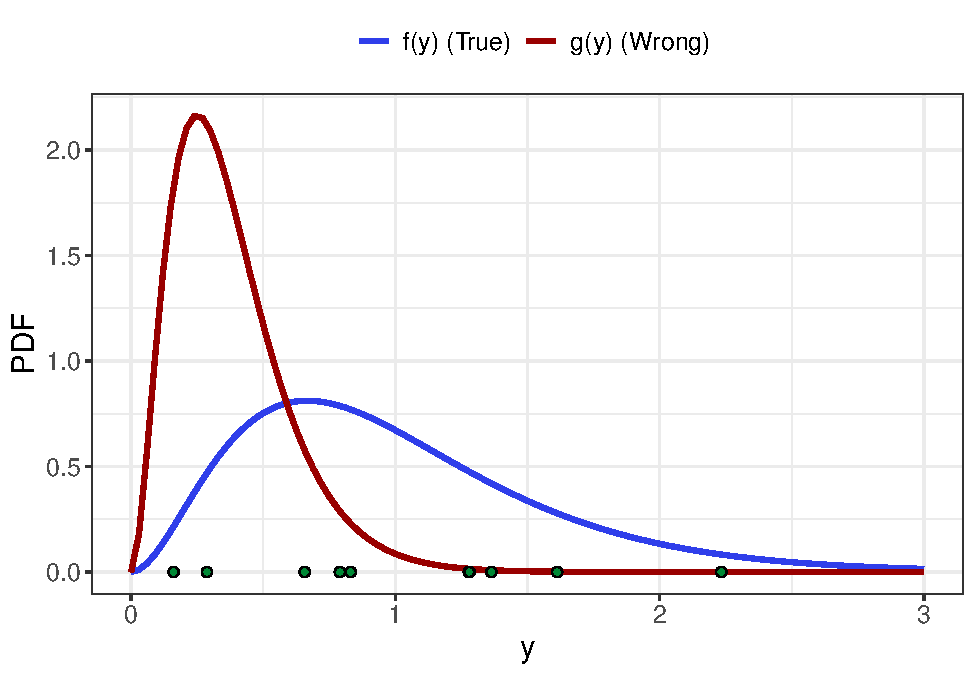
\includegraphics[width=1\linewidth]{_main_files/figure-latex/LogSExamplePlot-1} \caption{Observations (green dots) were simulated from a \(\G(3,3)\)-distribution. The true model \(f\) (blue) is shown, along with the PDF for the competing model \(g\), which follows a \(G(3,8)\)-distribution.}\label{fig:LogSExamplePlot}
\end{figure}

The logarithmic score of the true model \(f\) for the first observation, \(y_1=1.278\), is calculated as follows

\begin{equation}
  \begin{aligned}
  -\log\big(f(y_1)\big)&=-\log\big(f(1.278)\big) \\
  &=-\log\left[ \frac{1}{\Gamma(3)4}\Big(\frac{1.278}{4}\Big)^{3-1}\exp(-1.278/4)\right] \\
  &=-1.156
  \end{aligned}
\end{equation}

Similarly, the logarithmic scores for the other observations can be calculated using the same formula. The individual logarithmic scores for all 10 observations are presented in Table \ref{tab:tabLogS}. Among the 10 observations, 8 of them are more likely to occur under the true model \(f\) compared to the competing model \(g\). The final key quantity, the average logarithmic score, \(\bar{S}(G,\boldsymbol y)\), can be calculated using Equation \eqref{eq:averageLogS}.

\begin{equation}
  \begin{aligned}
    \bar{S}(f,\boldsymbol y) &=1.1 \\
    \bar{S}(g,\boldsymbol y) &=3.22
  \end{aligned}
\end{equation}

\begin{table}[H]

\caption{\label{tab:tabLogS}Logarithmic scores of the two different Gamma models w.r.t. the 10 individual observations.}
\centering
\begin{tabu} to \linewidth {>{\raggedright}X>{\raggedright}X>{\raggedright}X>{\raggedright}X>{\raggedright}X>{\raggedright}X>{\raggedright}X>{\raggedright}X>{\raggedright}X>{\raggedright}X>{\raggedright}X}
\toprule
$i$ & 1 & 2 & 3 & 4 & 5 & 6 & 7 & 8 & 9 & 10\\
$\bar{S}(f,y_i)$ & 1.16 & 3.86 & 0.00 & 0.23 & 1.16 & 0.18 & 1.37 & 2.03 & 0.17 & 0.83\\
$\bar{S}(g,y_i)$ & 4.19 & 10.71 & 0.55 & 1.47 & 4.21 & -0.75 & 4.74 & 6.40 & 1.25 & -0.60\\
\bottomrule
\end{tabu}
\end{table}

\end{example}

\cleardoublepage

\chapter{Case studies}

This chapter presents the findings obtained from applying both the state-of-the-art outbreak detection algorithm and the novel outbreak detection algorithm to the subset of diseases examined in this master's thesis. To demonstrate the practical application of these algorithms, a comprehensive case study focused on STEC will be presented as the primary focus. The results of the remaining case studies will be presented in a more concise manner to maintain reader engagement. However, for a complete collection of related figures and tables, please refer to Appendix \ref{FigAndTabCaseStudy}.

It is widely recognized that effective monitoring of a surveillance time series necessitates accurate modeling of the time series prior to assessing aberrations. Therefore, the performance of these algorithms in identifying outbreaks within the selected diseases will be thoroughly discussed and analyzed. Both the state-of-the-art algorithms and the novel algorithms take into account trends and seasonality, which will be addressed in the analysis.

Furthermore, a comprehensive comparative analysis will be conducted to provide valuable insights into the strengths and limitations of both the state-of-the-art algorithms and, more importantly, the novel algorithms.

For a detailed presentation of the data used to generate these results, please refer to Chapter \ref{Dataset}.

\section{Shiga toxin (verotoxin)-producing \textit{Escherichia coli}}

The initial analysis focuses on STEC. The data set comprises monthly counts of Danish STEC cases, denoted as \(y_{it}\), where \(i=1,\dots,6\) represents the six age groups and \(t=1,\dots,T\) represents the time period of \(T=180\) months starting in 2008. The first step involves applying the state-of-the-art outbreak detection algorithms to identify potential outbreaks in the time series.

Following that, the novel outbreak detection algorithm is utilized, and different models for the fixed effects are proposed. Both the hierarchical Poisson Normal model and the hierarchical Poisson Gamma model is considered for the modeling framework. The performance of these models is compared using the average logarithmic score, \(\bar{S}(G,y)\), to determine the most appropriate model for further analysis.

\subsection{Applying the state-of-the-art outbreak detection algorithm to Shiga toxin (verotoxin)-producing \textit{Escherichia coli}}

To investigate outbreak detection, the Farrington method and the Noufaily method, as described in Section \ref{StateOfTheArt}, are initially explored. These methods can be implemented using the \texttt{farringtonFlexible} function, which is available in the R package called \textbf{surveillance}. The specific \texttt{control} arguments for each method can be found in Appendix \ref{controlsStateOfTheArt}.

For this analysis, the reference values are based on data collected from January 2008 to February 2011. Subsequently, surveillance is performed using the data spanning from March 2011 to December 2022. The resulting time series is visualized in Figure \ref{fig:CompareStateOfTheArtSTEC}.



\begin{figure}[H]
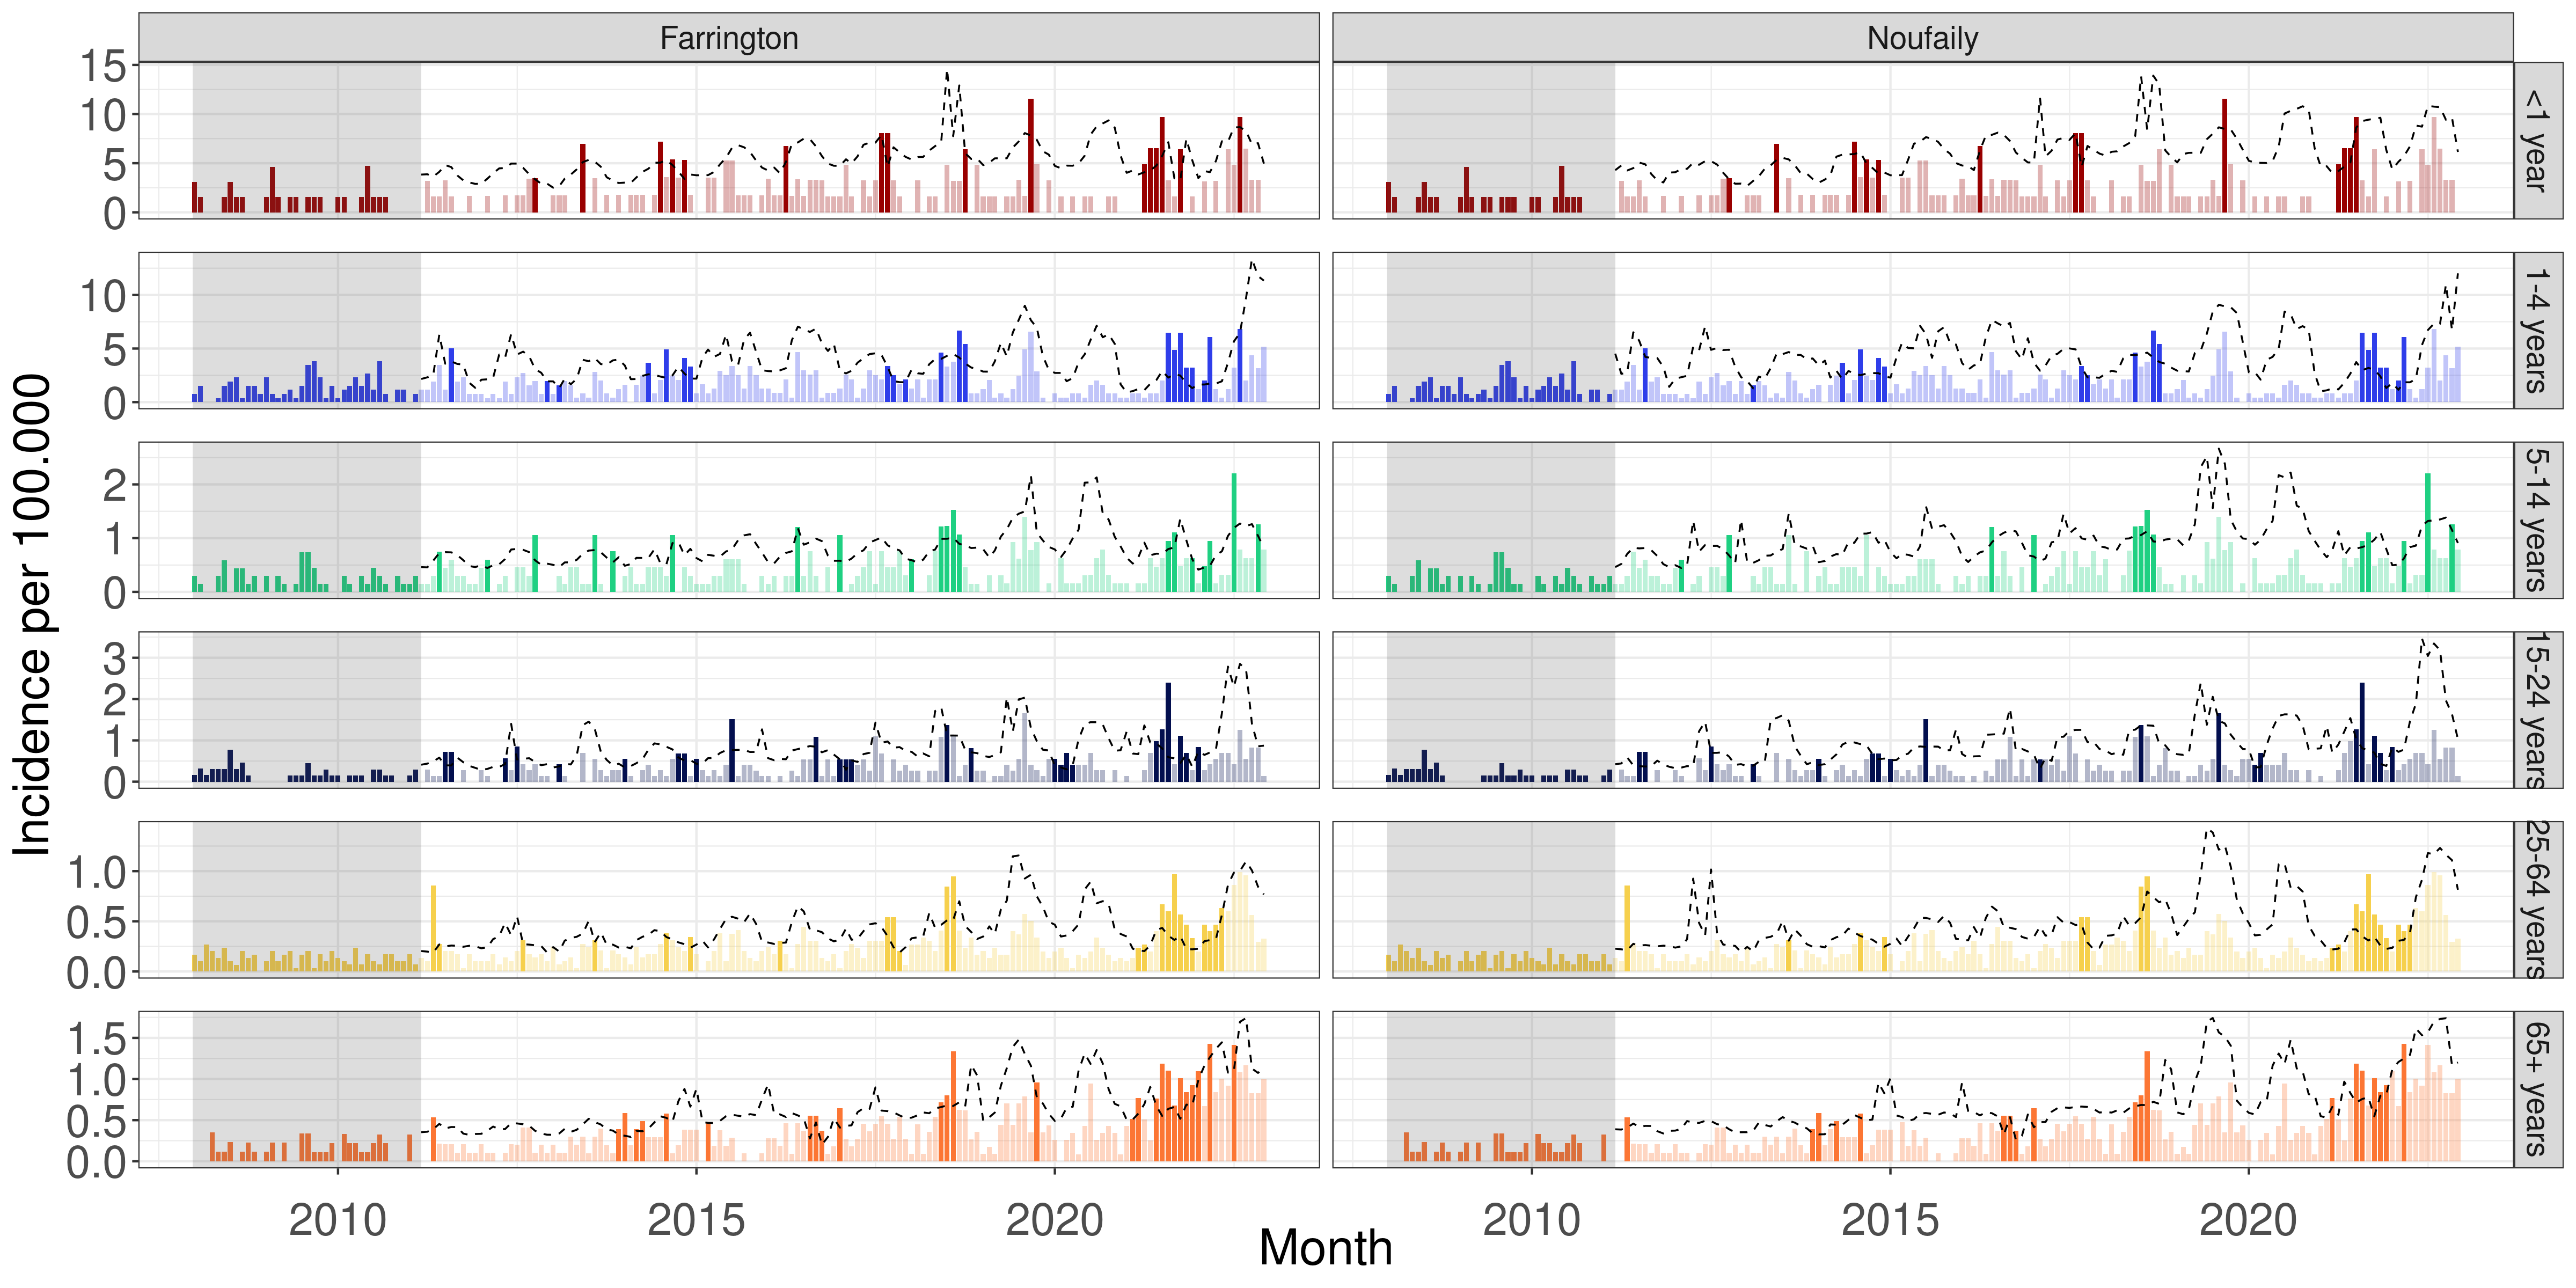
\includegraphics[width=1\linewidth]{../figures/Compare_stateOfTheArt_STEC} \caption{Monthly Shiga toxin (verotoxin)-producing \textit{Escherichia coli} incidence per 100.000 in Denmark, 2008-2022. Monitored by (left) Farrington and (right) Noufaily method. Reference data for the estimation of model parameters from January 2008 to March 2011 (grey area). Threshold (dashed line) is computed for observations timepoints outside reference data. Alarm triggered (dark color) if observations exceeds threshold.}\label{fig:CompareStateOfTheArtSTEC}
\end{figure}

Figure \ref{fig:CompareStateOfTheArtSTEC} displays multiple alarms for both the Farrington method and the Noufaily method. The Farrington method generates a total of 134 alarms, while the Noufaily method produces a significantly lower count of 101 alarms.

The substantial number of alarms generated by both the Farrington method and the Noufaily method raises valid concerns. The sheer volume of alarms can overwhelm epidemiologists, posing challenges in effectively prioritizing and investigating potential outbreaks. It is crucial to avoid reacting solely to individual alarms and instead consider the bigger picture.

Of particular importance are alarms that are triggered simultaneously in multiple age groups or during concurrent time points. Such patterns indicate potential outbreaks that warrant further attention and investigation by epidemiologists. By analyzing and interpreting the alarms in context, epidemiologists can gain a more comprehensive understanding of the outbreak situation and make informed decisions about resource allocation and intervention strategies.

\subsection{Applying the novel outbreak detection algorithm to Shiga toxin (verotoxin)-producing \textit{Escherichia coli}}

The subsequent investigation focuses on the application of the novel outbreak detection algorithm to analyze outbreaks. In this analysis, a rolling window with a width of \(k=36\) is selected. The reference values are established using monthly data collected from January 2008 to December 2010. Subsequently, the time series is monitored using data from January 2011 to December 2022.

To identify outbreaks, an observation is classified as such if the one-step ahead random effect \(u_{t_1}\) exceeds the upper bound \(U_{t_0}\). The upper bound is determined as the 90\% quantile of the distribution of random effects obtained from the second stage model. This threshold helps identify significant deviations in the outbreak intensity.

To ensure effective monitoring, a series of models for the fixed effects are proposed, with each model building upon the previous one. These models aim to capture different aspects of the disease dynamics and improve the accuracy of outbreak detection.

In the initial model, the intensity \(\lambda_{it}\) is assumed to be solely dependent on the age group and the population size \(n_{it}\). The model is formulated as:

\begin{equation}\label{eq:Agegroup}
  \log(\lambda_{it}) = \beta(ageGroup_{i}) + \log(n_{it})
\end{equation}

Here, \(\beta(ageGroup_{i})\) represents the fixed effect specific to the age group \(i\), capturing the age group's influence on the outbreak intensity. The term \(\log(n_{it})\) acts as an offset, accounting for the population size at time \(t\) for age group \(i\).

In the first extension of this initial model, the trend over time across all age groups is incorporated. The extended model is formulated as:

\begin{equation}
  \log(\lambda_{it})=\beta(ageGroup_{i}) + \beta_{trend} t + \log(n_{it})
\end{equation}

In this model, \(\beta_{trend}\) quantifies the rate of change in the outbreak intensity over time. By including this parameter, the model accounts for the overall trend in the outbreak intensity across all age groups, allowing for a more comprehensive analysis of the outbreak dynamics.

In addition to the models described earlier, another model is proposed, which incorporates seasonality into the analysis. This model builds upon the initial model and assumes an annual seasonality pattern. The intensity \(\lambda_{it}\) is modeled as follows:

\begin{equation}
\log(\lambda_{it})=\beta(ageGroup_{i})+ \sin \big(\frac{2\pi\cdot \tau_t}{12}\big) \beta_{\sin} + \cos \big(2\frac{\pi\cdot \tau_t}{12}\big) \beta_{\cos} + \log(n_{it})
\end{equation}

In this model, \(\tau_t\) represents the time period \(t\) within a year, ranging from 1 to 12 (corresponding to the months of January to December). The parameters \(\beta_{\sin}\) and \(\beta_{\cos}\) capture the effect of the seasonal pattern on the outbreak intensity. By including sine and cosine functions of \(\tau_t\), the model accounts for the periodic fluctuations in the outbreak intensity observed throughout the year. This allows for the detection and analysis of seasonality patterns in the outbreak data, providing insights into the seasonal variations in disease occurrence.

In addition to the models described earlier, a final model is proposed that combines both trend and seasonality components. This model builds upon the previous models and includes the effects of both the overall trend over time and the seasonal patterns. The intensity \(\lambda_{it}\) is modeled as follows:

\begin{equation}\label{eq:AgegroupTrendSeasonality}
  \log(\lambda_{it})=\beta(ageGroup_{i}) + \beta_{trend} t + \sin \big(\frac{2\pi\cdot \tau_t}{12}\big) \beta_{\sin} + \cos \big(\frac{2\pi\cdot \tau_t}{12}\big)\beta_{\cos} + \log(n_{it})
\end{equation}

The proposed models above are subsequently implemented and estimated in two different modeling frameworks: the hierarchical Poisson Normal model and the hierarchical Poisson Gamma model. The goodness-of-fit of these models is evaluated using the average logarithmic score, \(\bar{S}(G,y)\). An excerpt of these results, namely for the models with the lowest logarithmic score, \(\bar{S}(G,y)\), for both modeling frameworks, are summarized in Table \ref{tab:STECNovelTbl}. For the full table of results, refer to Table \ref{tab:STECNovelTblAppendix}.

\begin{longtable}[t]{lrll}
\caption{\label{tab:STECNovelTbl}The average logarithmic score, $\bar{S}(G, y)$, is computed for the model described in  \eqref{eq:AgegroupTrendSeasonality} that models Shiga toxin (verotoxin)-producing \textit{Escherichia coli}. The parameter estimates at time $t_0$ are also obtained for this model. Both the hierarchical Poisson Normal model and the hierarchical Poisson Gamma model are considered for the analysis. Confidence intervals for the parameter estimates are calculated using profile likelihood confidence intervals.}\\
\toprule
 & $\bar{S}(G,y)$ & Parameter & Estimate (95\% CI)\\
\midrule
\endfirsthead
\caption[]{\textit{(continued)}}\\
\toprule
Model & $\bar{S}(G,y)$ & Parameter & Estimate (95\% CI)\\
\midrule
\endhead

\endfoot
\bottomrule
\endlastfoot
\addlinespace[0.3em]
\multicolumn{4}{l}{\textit{\textbf{Poisson Normal}}}\\
\hspace{1em} & 13.12 & $\beta_{trend}$ & 0.04 (0.03, 0.05)\\

\hspace{1em} &  & $\beta_{<1 year}$ & 11.95 (11.68, 12.31)\\

\hspace{1em} &  & $\beta_{1-4 years}$ & 14.51 (14.28, 14.73)\\

\hspace{1em} &  & $\beta_{5-14 years}$ & 15 (14.75, 15.26)\\

\hspace{1em} &  & $\beta_{15-24 years}$ & 15.42 (15.19, 15.66)\\

\hspace{1em} &  & $\beta_{25-64 years}$ & 17.82 (17.64, 18.03)\\

\hspace{1em} &  & $\beta_{65+ years}$ & 16.59 (16.4, 16.81)\\

\hspace{1em} &  & $\beta_{\sin}$ & -0.33 (-0.43, -0.21)\\

\hspace{1em} &  & $\beta_{\cos}$ & -0.22 (-0.33, -0.1)\\

\hspace{1em} &  & $\log(\sigma)$ & -1.1 (-1.45, -0.87)\\
\cmidrule{1-4}
\addlinespace[0.3em]
\multicolumn{4}{l}{\textit{\textbf{Poisson Gamma}}}\\
\hspace{1em} & 13.13 & $\beta_{trend}$ & 0.04 (0.03, 0.05)\\

\hspace{1em} &  & $\beta_{<1 year}$ & 12.06 (11.74, 12.35)\\

\hspace{1em} &  & $\beta_{1-4 years}$ & 14.58 (14.36, 14.8)\\

\hspace{1em} &  & $\beta_{5-14 years}$ & 15.06 (14.81, 15.31)\\

\hspace{1em} &  & $\beta_{15-24 years}$ & 15.48 (15.25, 15.71)\\

\hspace{1em} &  & $\beta_{25-64 years}$ & 17.88 (17.69, 18.07)\\

\hspace{1em} &  & $\beta_{65+ years}$ & 16.65 (16.45, 16.85)\\

\hspace{1em} &  & $\beta_{\sin}$ & -0.32 (-0.43, -0.21)\\

\hspace{1em} &  & $\beta_{\cos}$ & -0.21 (-0.32, -0.1)\\

\hspace{1em} &  & $\log(\phi)$ & -2.29 (-2.95, -1.77)\\*
\end{longtable}

The models incorporating both trends and seasonality have shown improved performance in terms of lower logarithmic scores, indicating a better fit to the data. As a result, these models have been selected for further investigation regarding their ability to detect outbreaks.

Additionally, it is worth noting that the parameter estimates and confidence intervals for the fixed effects are consistent across the two modeling frameworks, despite the differences in assumptions about the distribution of random effects. This suggests that the choice of modeling framework does not have a substantial impact on the estimation of the fixed effects in this analysis.

Figure \ref{fig:CompareNovelSTEC} shows the one-step ahead random effects \(u_{i{t_1}}\) for each age group and the corresponding upper bounds \(U_{t_0}\) for both modeling frameworks.

The random effects \(u_{i{t_1}}\) represent the deviations from the expected outbreak intensity in the subsequent time period for each age group. These random effects provide information on whether there is an unusual or unexpected increase or decrease in the outbreak intensity compared to the expected values.

The upper bounds \(U_{t_0}\) are calculated based on the 90\% quantile of the distribution of the random effects obtained from the second stage model. They serve as threshold values to identify potential outbreaks. If the one-step ahead random effects exceed the upper bounds, it suggests a significant deviation from normal variation and indicates a potential outbreak.

By visualizing the one-step ahead random effects and the upper bounds together, epidemiologists can easily identify periods or age groups where the random effects surpass the upper bounds, highlighting potential outbreaks that require further investigation and monitoring.

is computed for the model described in \textbackslash eqref\{eq:AgegroupTrendSeasonality\}



\begin{figure}[H]
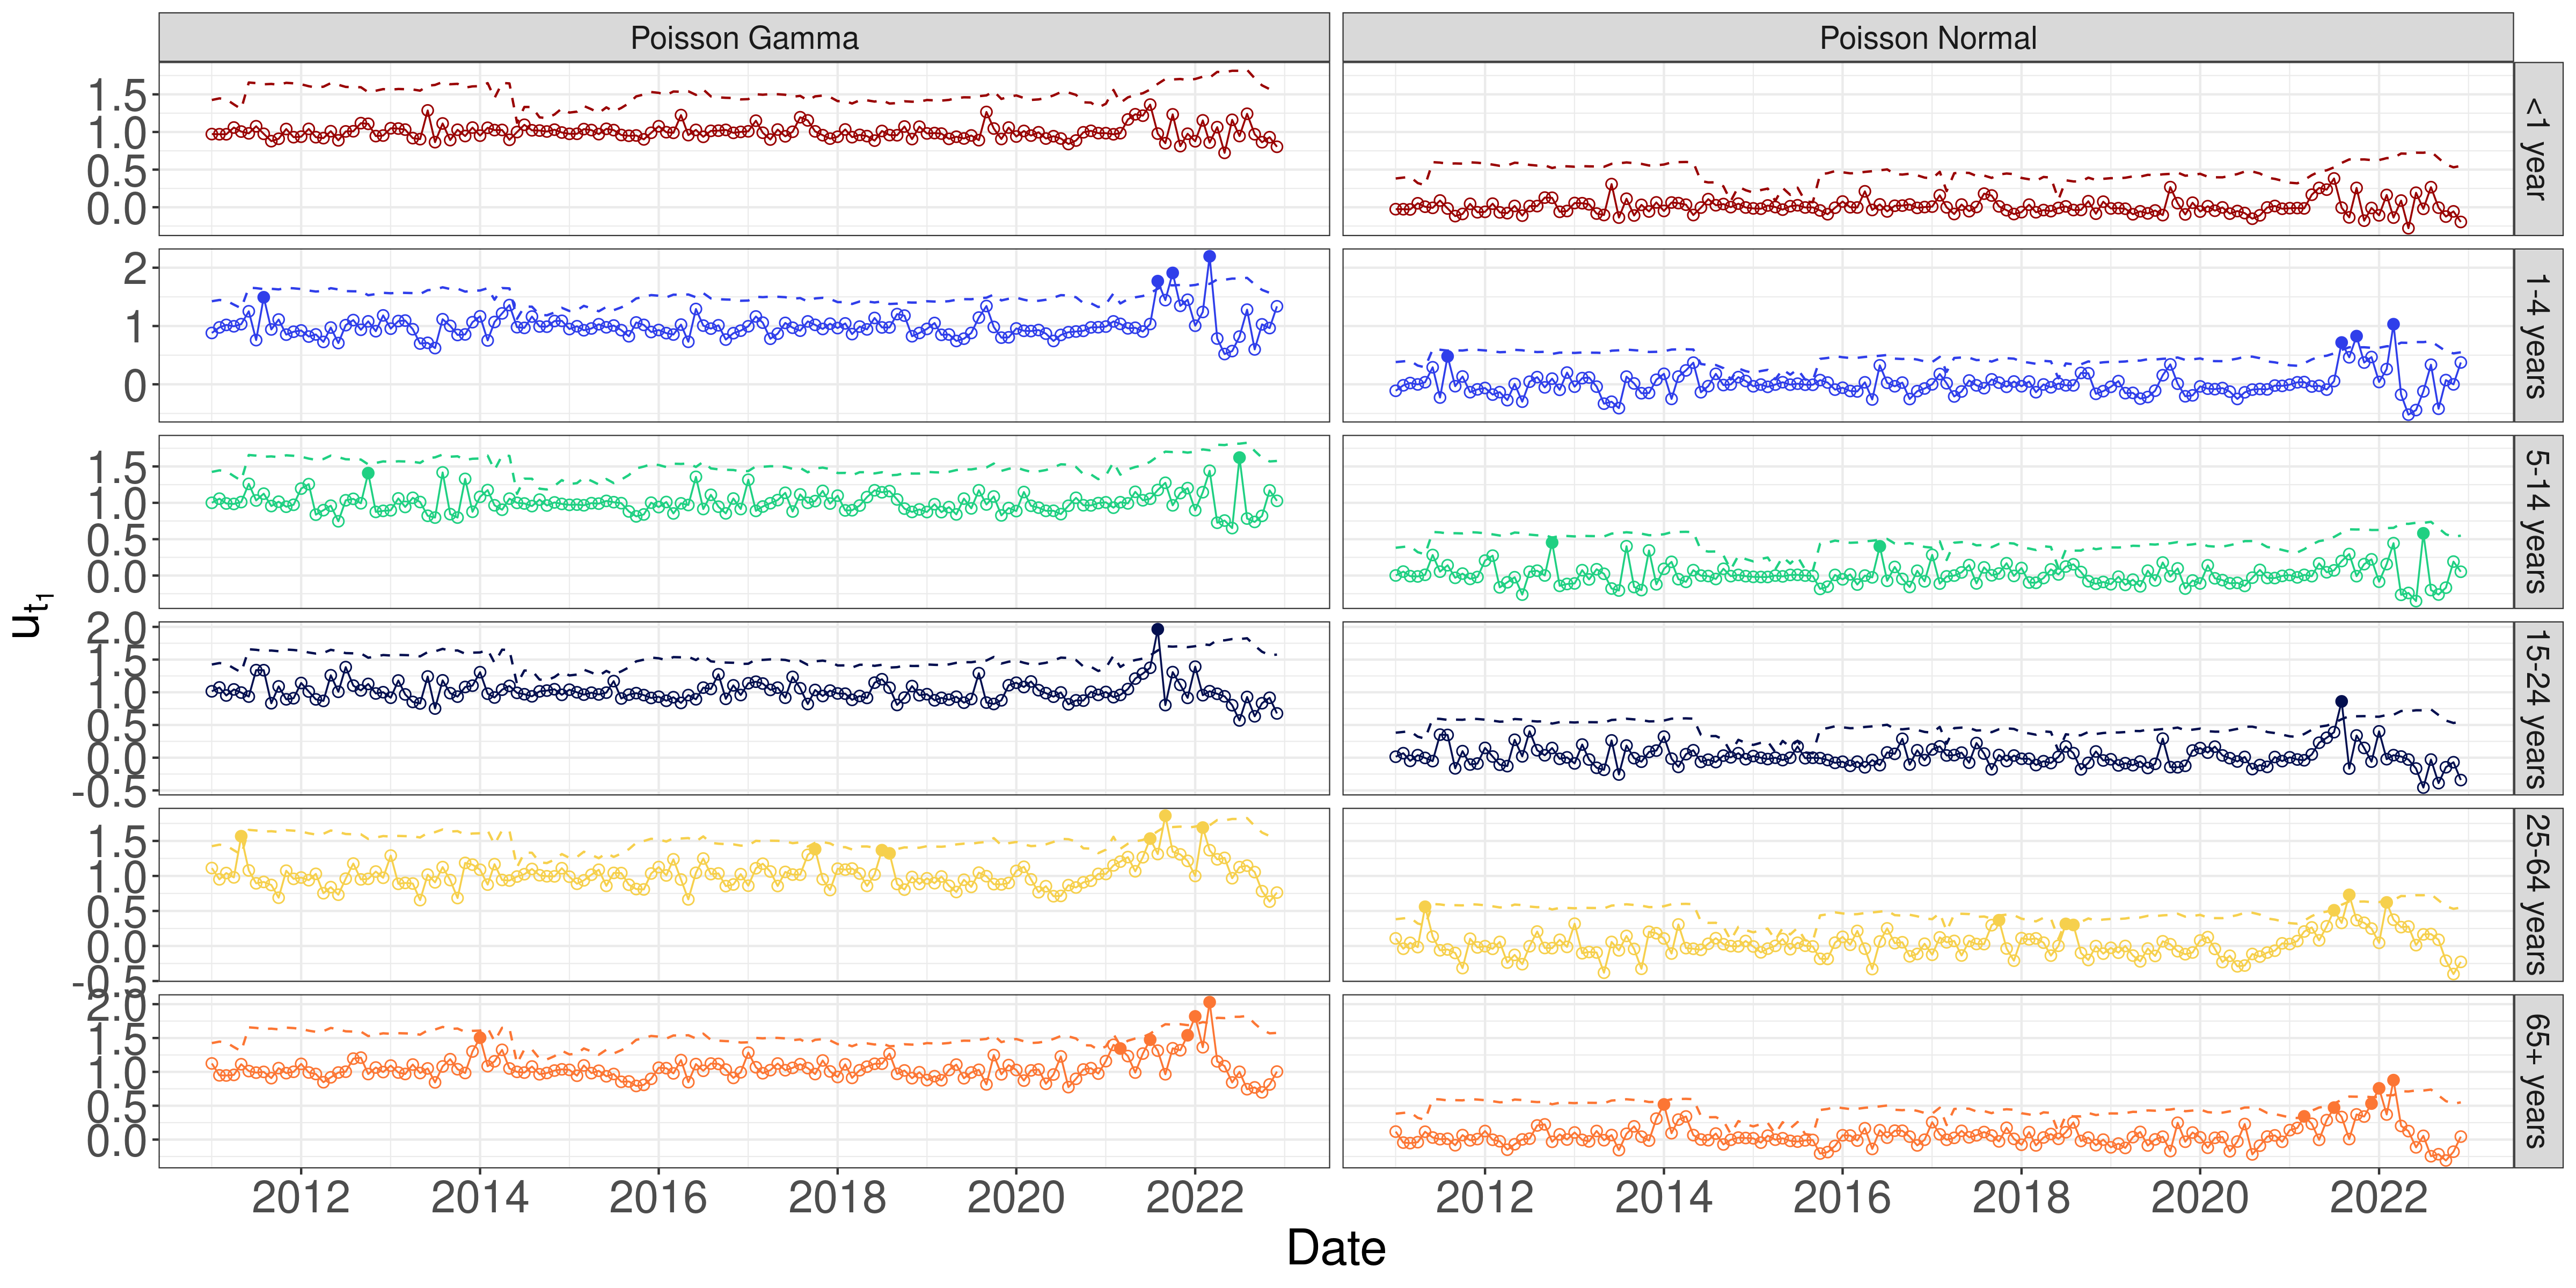
\includegraphics[width=1\linewidth]{../figures/Compare_novel_STEC} \caption{One-step ahead random effects \(u_{t_1}\) (circles) given the model described in \eqref{eq:AgegroupTrendSeasonality} for Shiga toxin (verotoxin)-producing \textit{Escherichia coli} in Denmark, 2011-2022. Poisson Normal model (right) and Poisson Gamma model (left) monitor the disease. Alarm raised (solid circle) if \(u_{t_1}\) exceeds the threshold (dashed line).}\label{fig:CompareNovelSTEC}
\end{figure}

SKRIVE HER NÅR RESULTATER ER FÆRIGE



\begin{figure}[H]
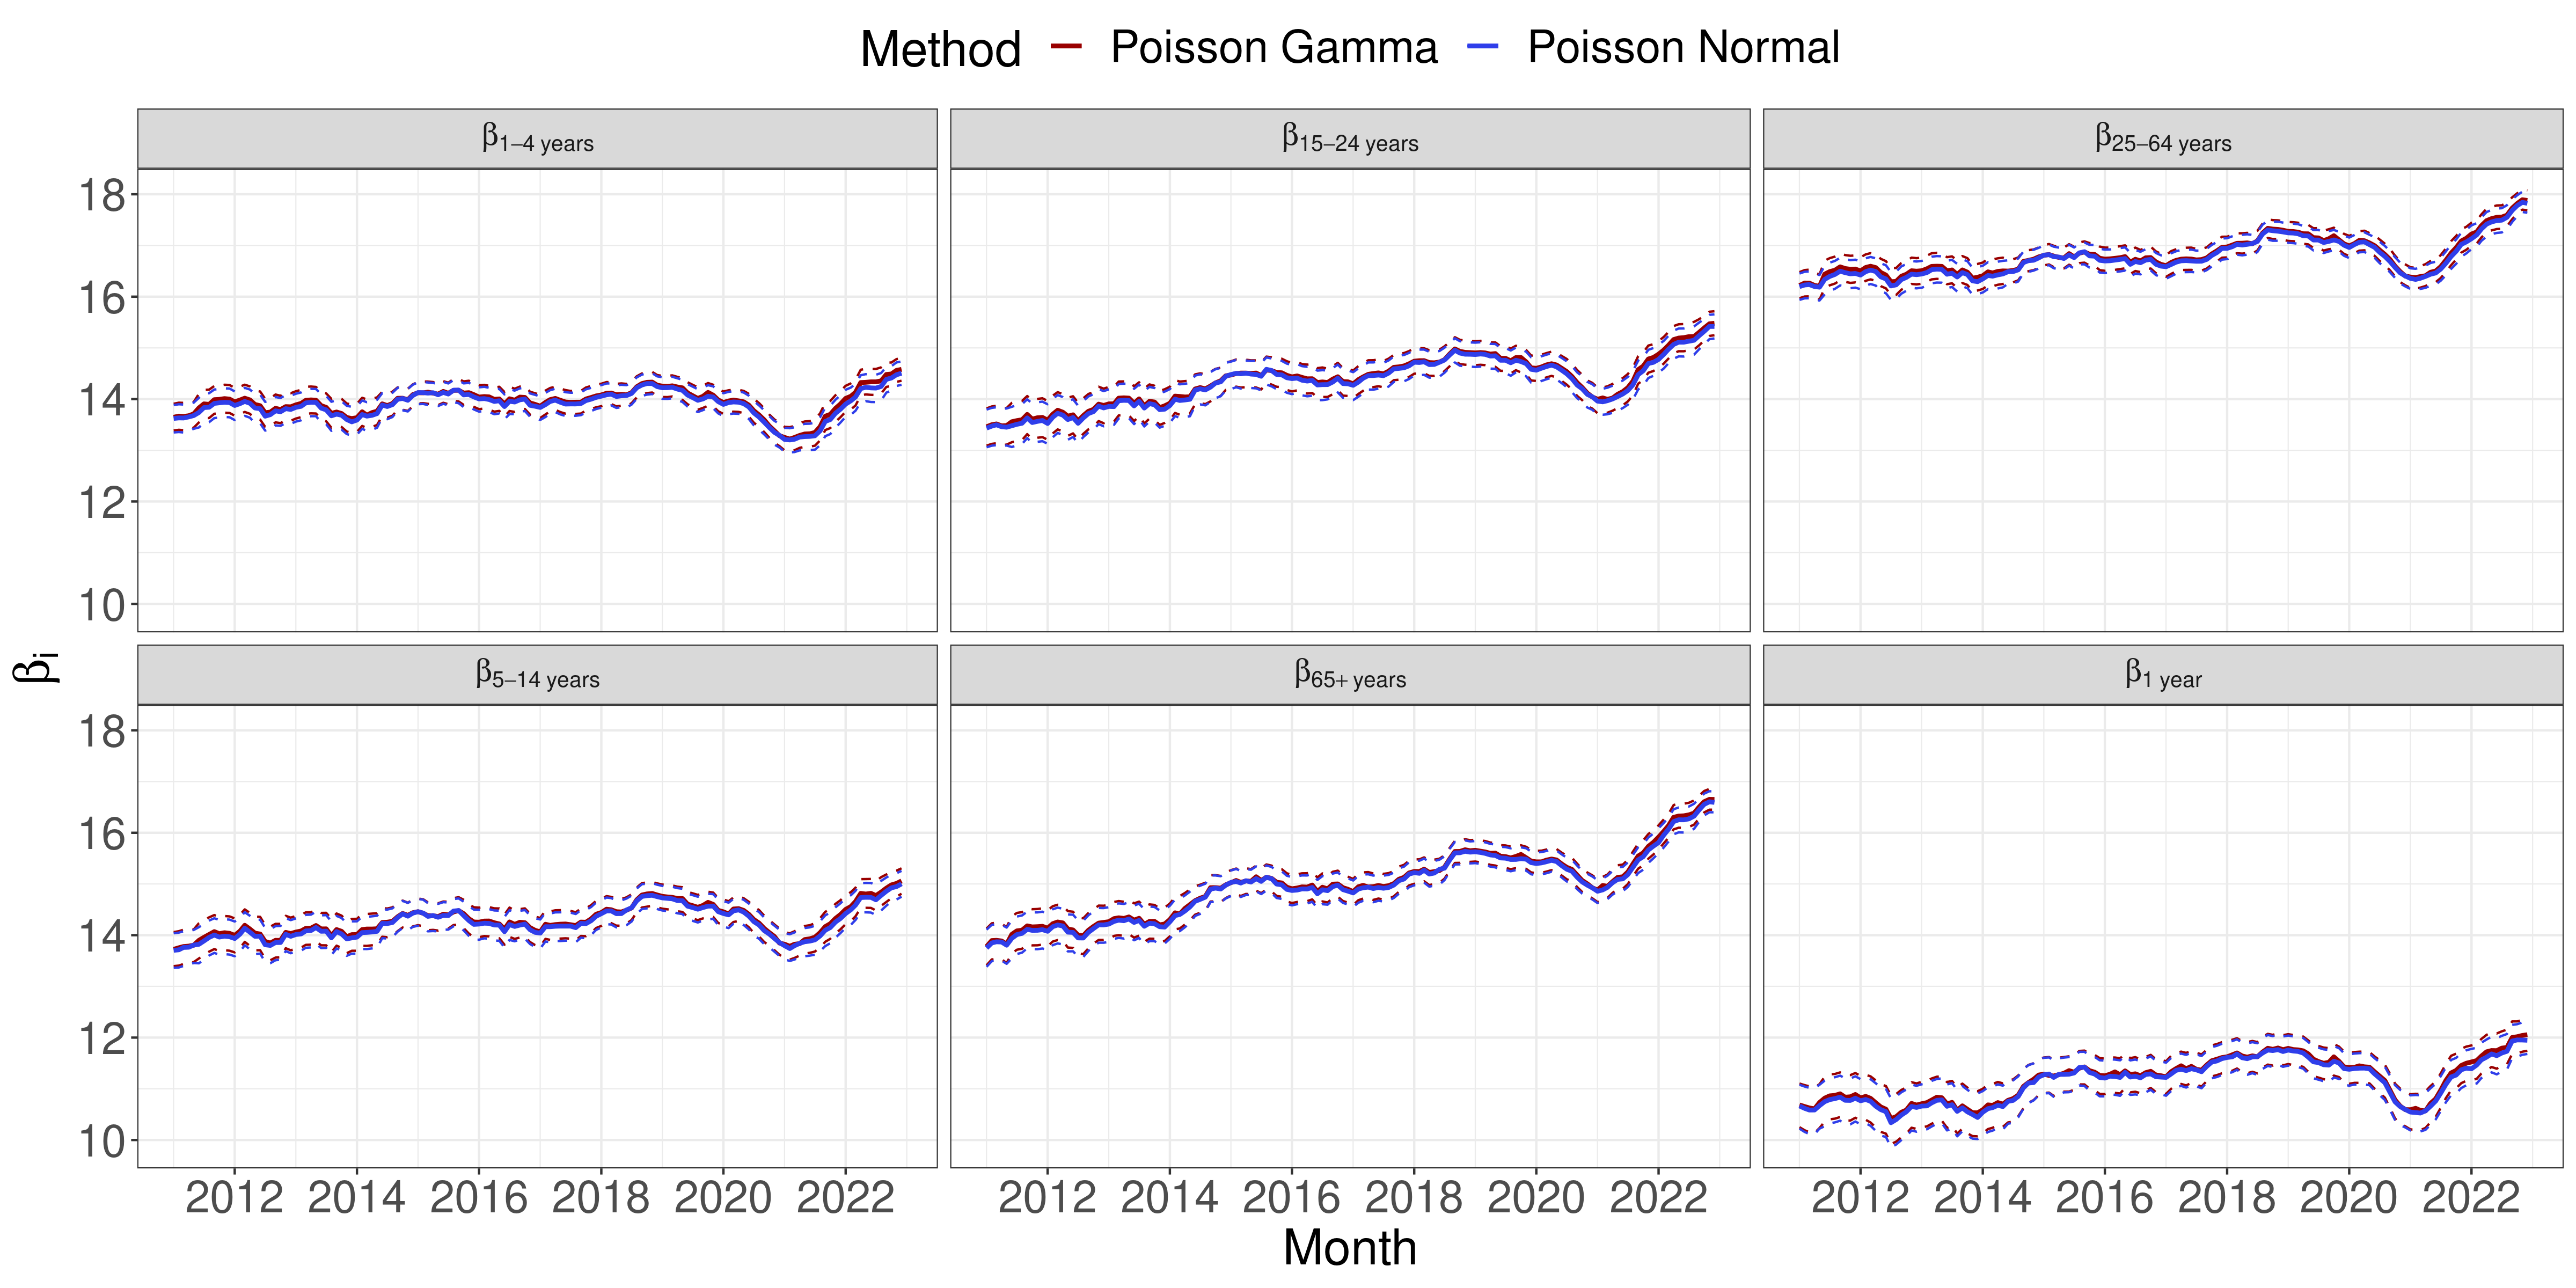
\includegraphics[width=1\linewidth]{../figures/STEC_novel_par_ageGroup} \caption{Estimates (solid line) and 95\% profile likelihood confidence intervals (dashed line) of \(\beta(ageGroup_i)\) are shown using a rolling window with a width of \(k=36\) for the time period between January 2011 and December 2022 for Shiga toxin (verotoxin)-producing \textit{Escherichia coli}.}\label{fig:STECnovelparageGroup}
\end{figure}



\begin{figure}[H]
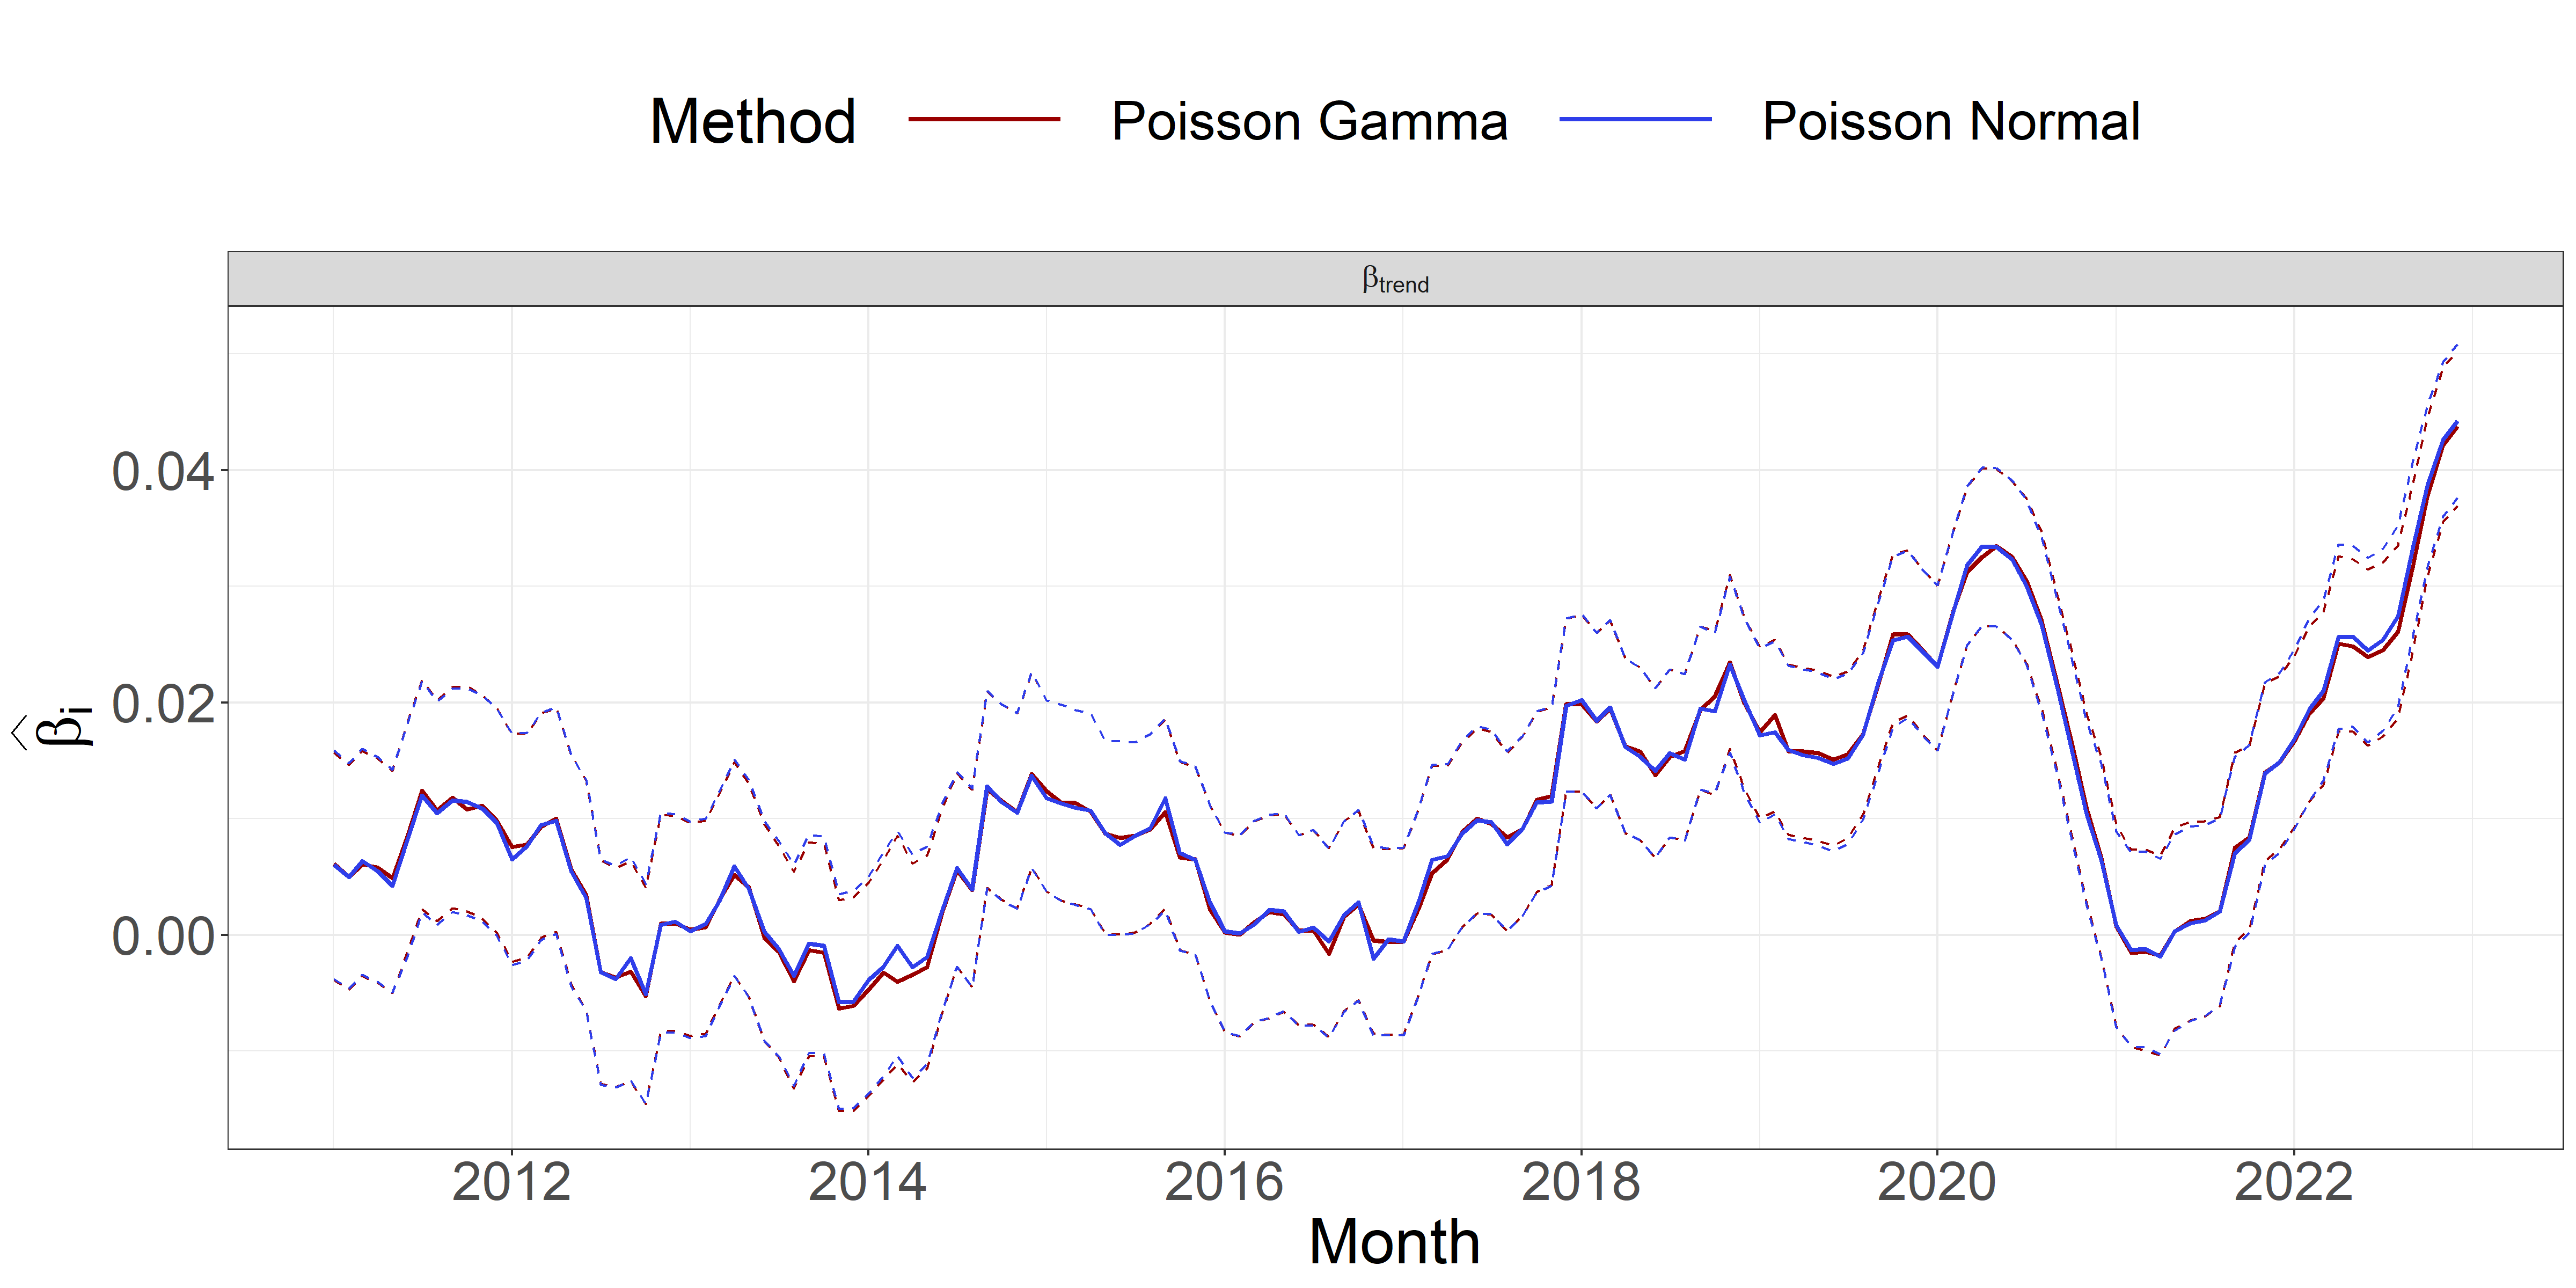
\includegraphics[width=1\linewidth]{../figures/STEC_novel_par_trend} \caption{Estimates (solid line) and 95\% profile likelihood confidence intervals (dashed line) of \(\beta_{\sin}\) and \(beta_{\cos}\) are shown using a rolling window with a width of \(k=36\) for the time period between January 2011 and December 2022 for Shiga toxin (verotoxin)-producing \textit{Escherichia coli}.}\label{fig:STECnovelpartrend}
\end{figure}



\begin{figure}[H]
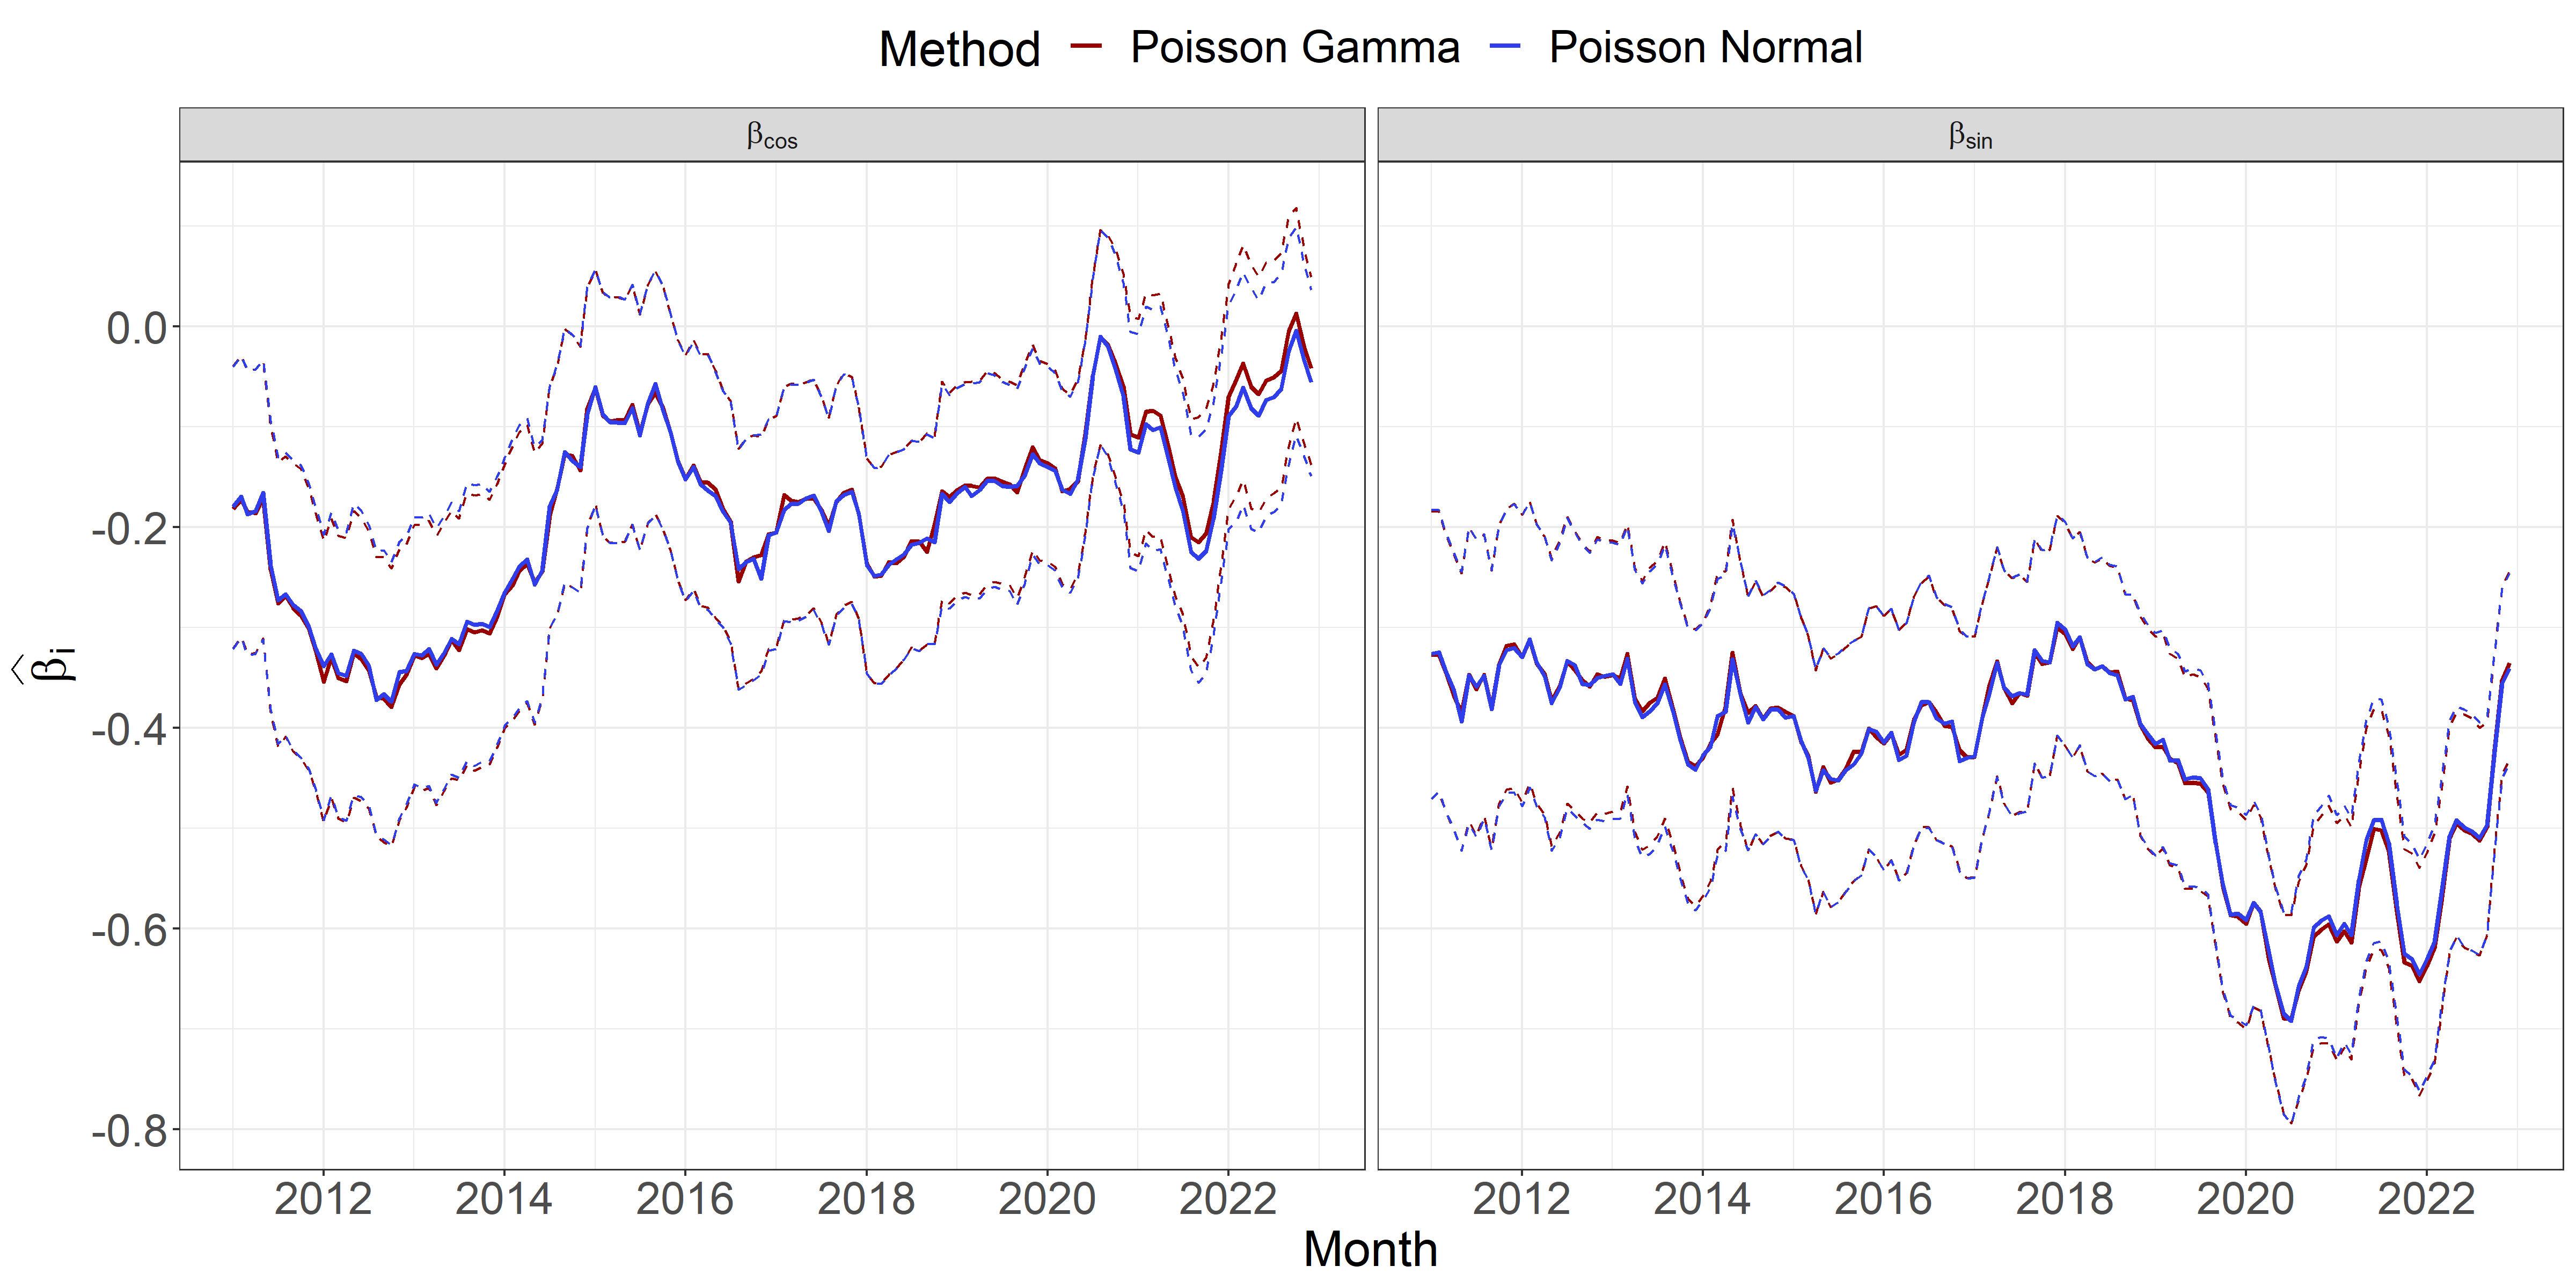
\includegraphics[width=1\linewidth]{../figures/STEC_novel_par_seasonality} \caption{Estimates (solid line) and 95\% profile likelihood confidence intervals (dashed line) of \(\beta_{trend}\) are shown using a rolling window with a width of \(k=36\) for the time period between January 2011 and December 2022 for Shiga toxin (verotoxin)-producing \textit{Escherichia coli}.}\label{fig:STECnovelparseasonality}
\end{figure}

Apart from the Poisson Gamma model being seemingly more robust, the estimated fixed effects parameters for the models are on a comparable scale. This can be seen in Figure \ref{fig:STECnovelparageGroup}



\begin{figure}[H]
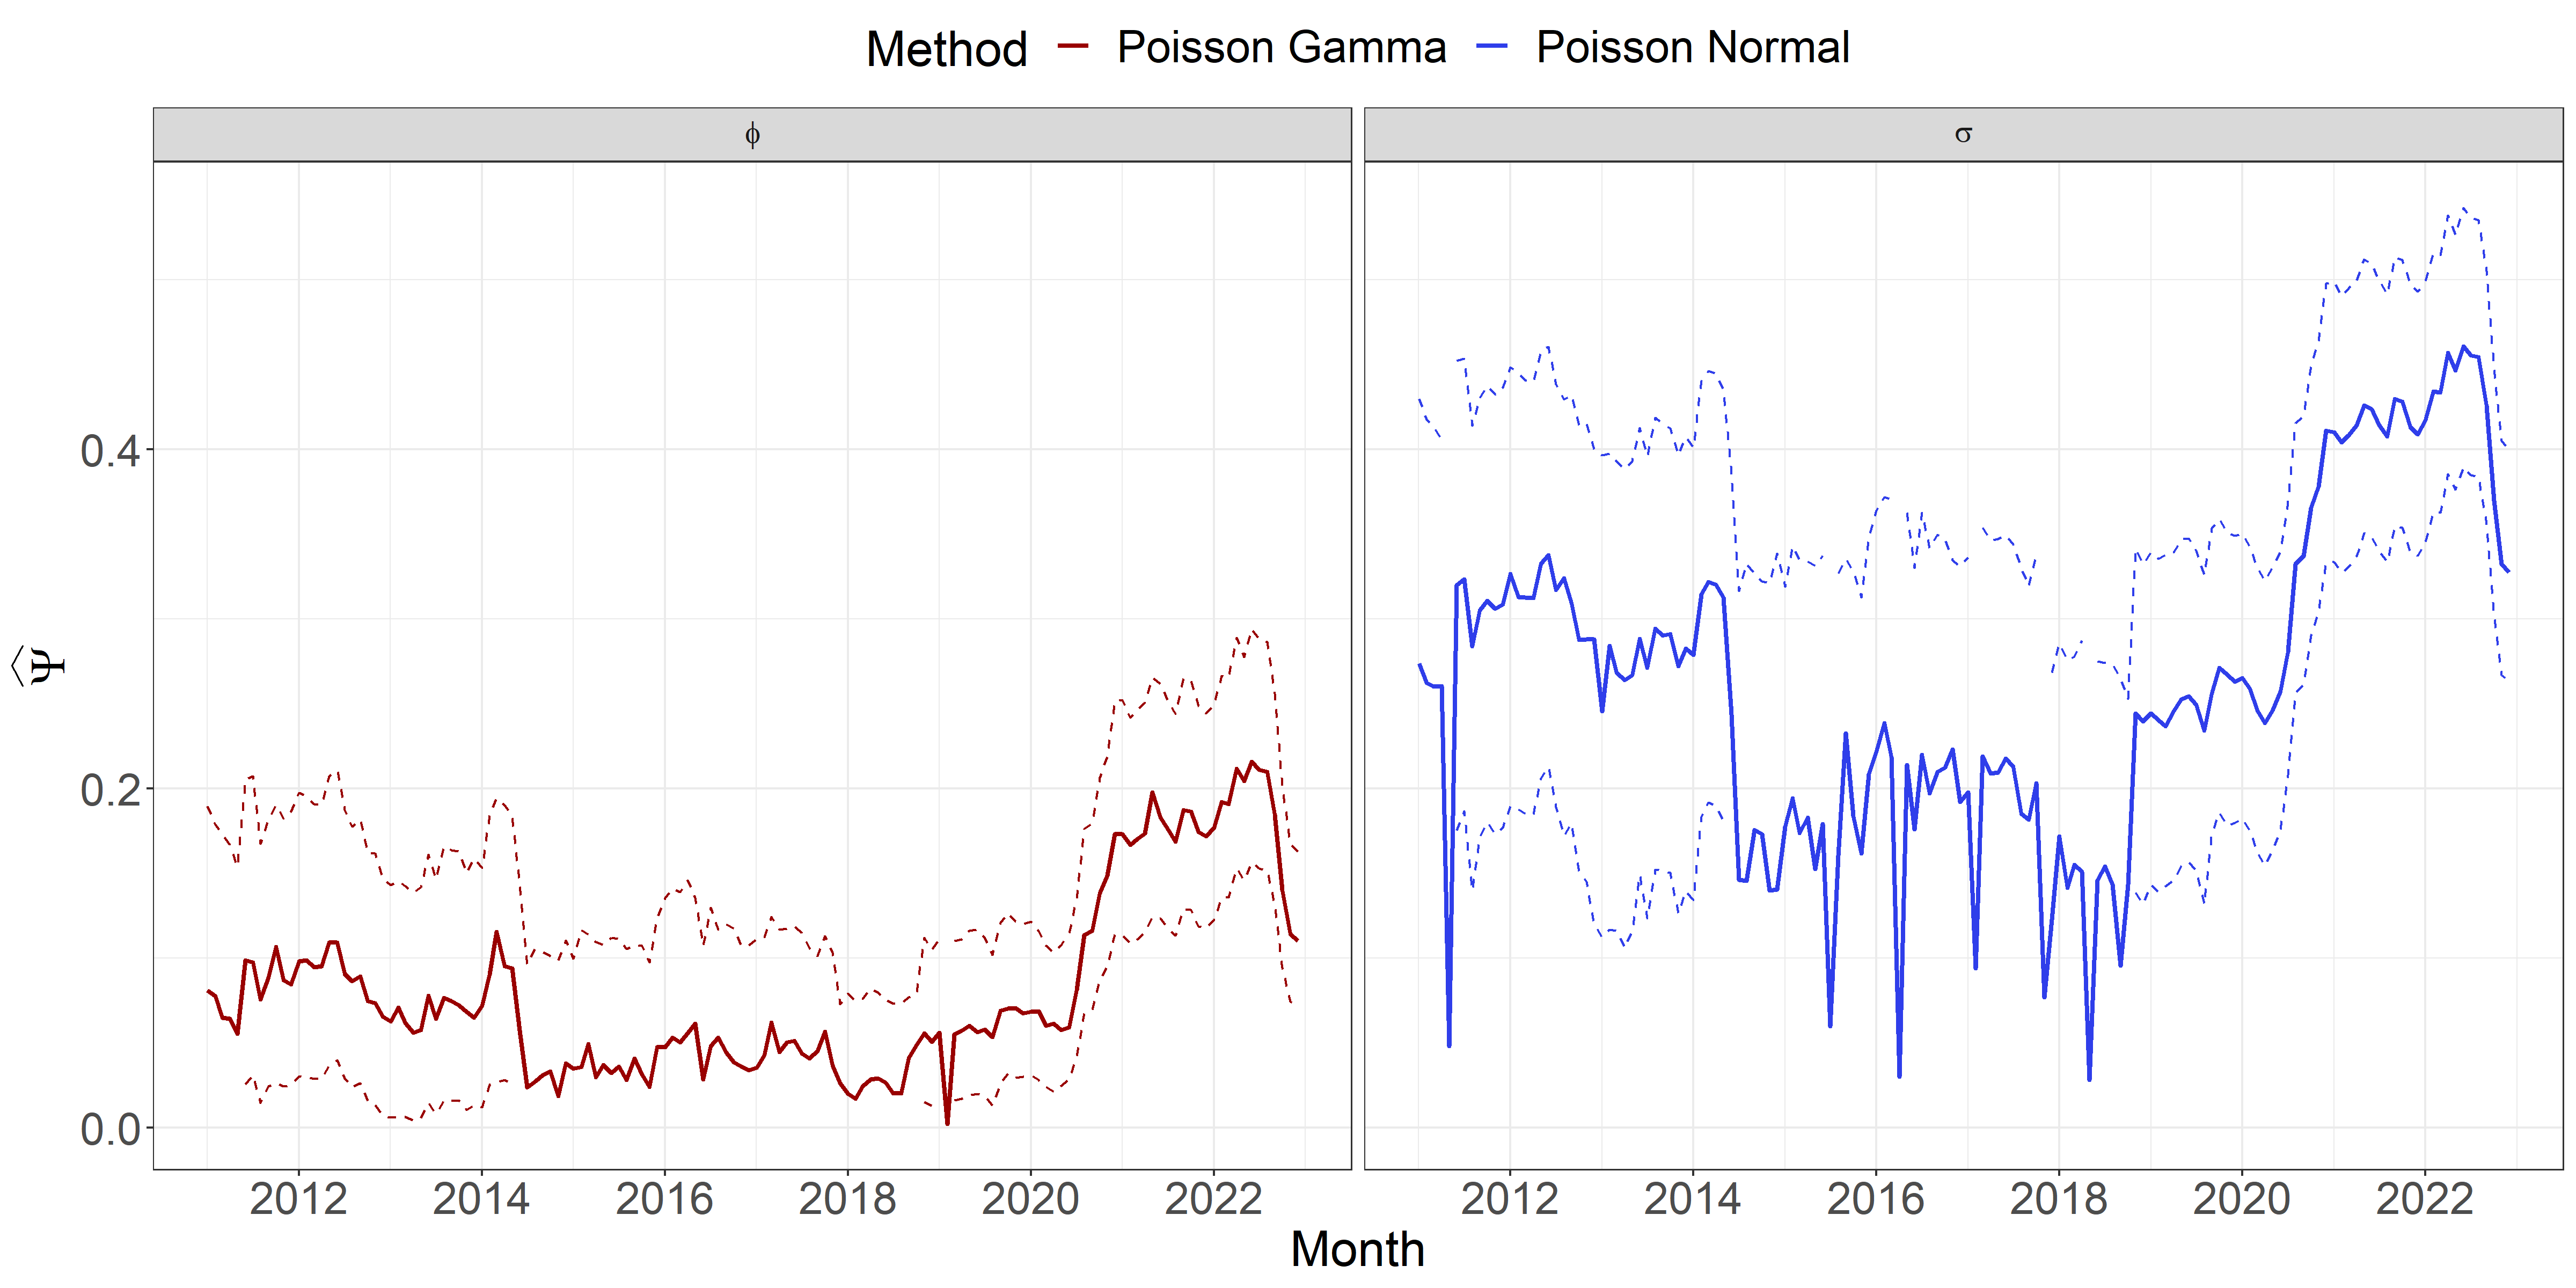
\includegraphics[width=1\linewidth]{../figures/STEC_novel_par_dispersion} \caption{Estimates (solid line) and 95\% profile likelihood confidence intervals (dashed line) of \(\phi\) and \(\sigma\) are shown using a rolling window with a width of \(k=36\) for the time period between January 2011 and December 2022 for Shiga toxin (verotoxin)-producing \textit{Escherichia coli}.}\label{fig:STECnovelparseaDispersion}
\end{figure}

\section{\textit{Listeriosis}}

Intuitively, it is not common to employ statistical methods for monitoring and detecting outbreaks of \textit{Listeriosis}. The current state-of-the-art approach for detecting outbreaks of this disease relies on laboratory-based methods, specifically WGS. WGS enables epidemiologists to link cases that have occurred over an extended period, even months or years apart, and identify them as part of a continuous-source outbreak. Statistical methods may face challenges in detecting such outbreaks due to their complex and prolonged nature. However, it is crucial to include this case study in the master's thesis to highlight both the strengths and limitations of the proposed method.

The data set used in this case study consists of monthly counts of Danish listeria cases, denoted as \(y_{it}\). The subscript \(i\) distinguishes between two age groups, with \(i=1\) representing the age group below 65 years and \(i=2\) representing the age group above 65 years. The subscript \(t\) represents the time period, ranging from \(t=1,\cdots,T\), where \(T=180\) corresponds to the total number of months starting in 2008.

Both the state-of-the-art outbreak detection algorithm and the novel outbreak detection algorithm are applied to this data set.

\subsection{Applying the state-of-the-art outbreak detection algorithm to \textit{Listeriosis}}

In Figure \ref{fig:CompareStateOfTheArtLIST}, multiple alarms can be observed for both the Farrington method and the Noufaily method. The Farrington method triggers a total of 28 alarms, while the Noufaily method produces slightly fewer alarms, specifically 25 alarms.

Initially, outbreak detection using the Farrington method and the Noufaily method, described in Section \ref{StateOfTheArt}, are investigated.

The reference values for the analysis are based on the data from January 2008 to February 2011. Subsequently, surveillance is conducted using the data from March 2011 to December 2021. The resulting series is visualized in Figure \ref{fig:CompareStateOfTheArtLIST}.



\begin{figure}[H]
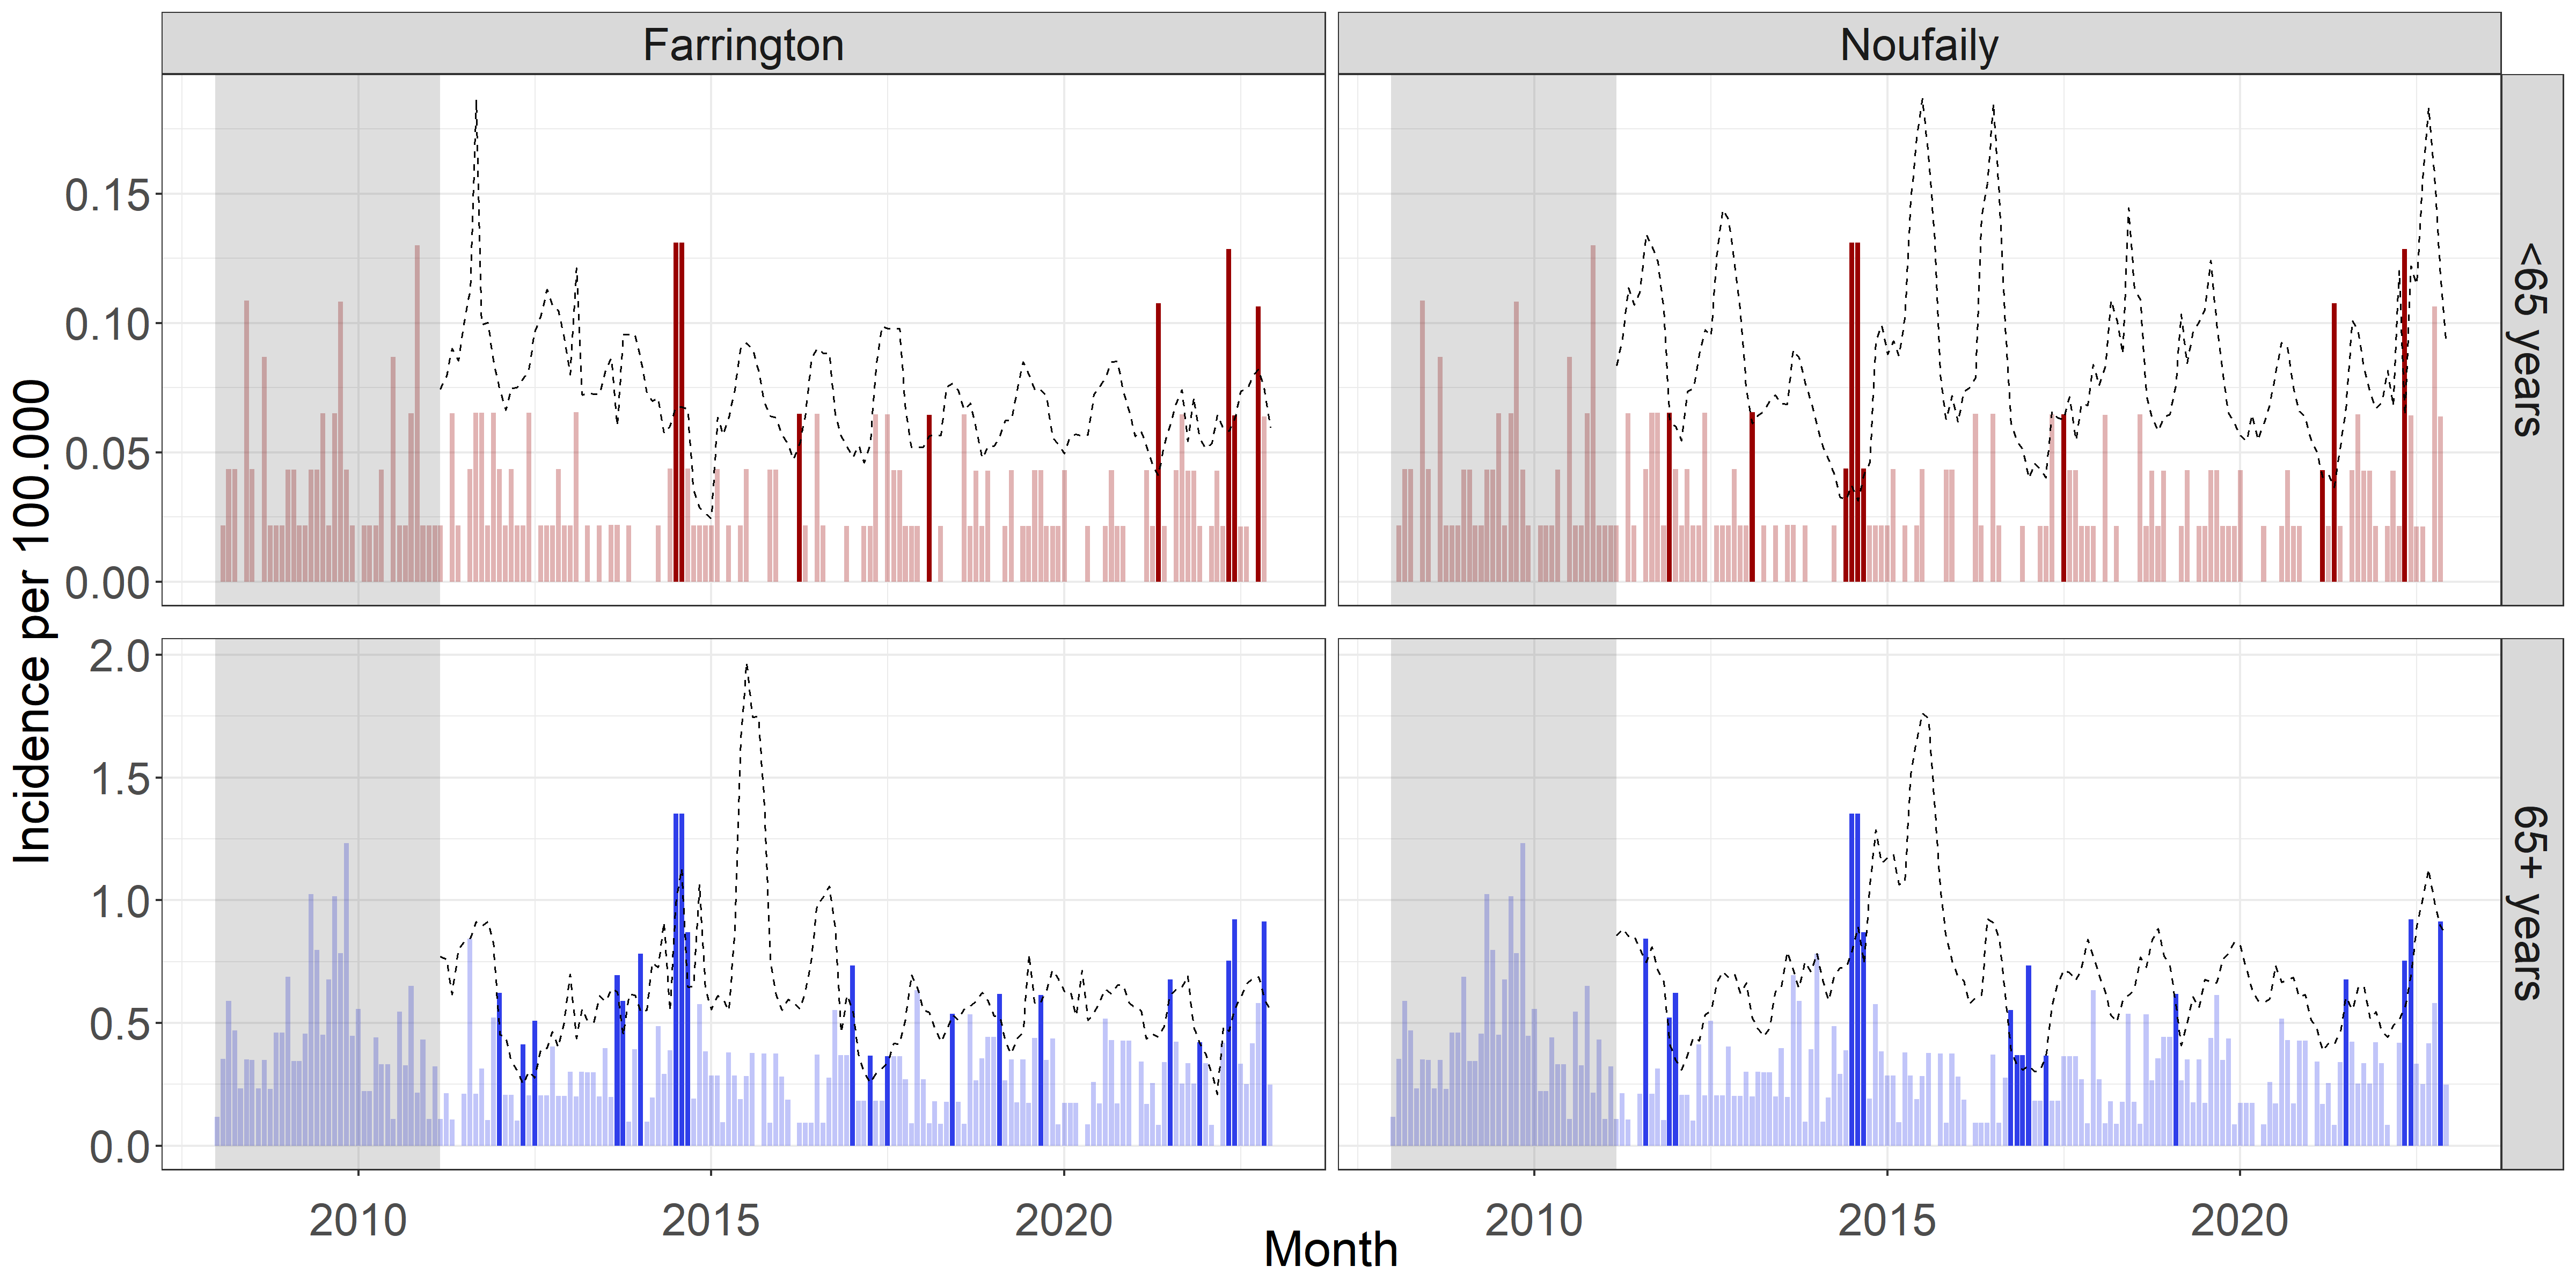
\includegraphics[width=1\linewidth]{../figures/Compare_stateOfTheArt_LIST} \caption{One-step ahead random effects \(u_{t_1}\) (circles) given the model described in \eqref{eq:Agegroup} for \textit{Listeriosis} in Denmark, 2011-2022. Poisson Normal model (right) and Poisson Gamma model (left) monitor the disease. Alarm raised (solid circle) if \(u_{t_1}\) exceeds the threshold (dashed line).}\label{fig:CompareStateOfTheArtLIST}
\end{figure}

Interestingly, both the Farrington method and the Noufaily method demonstrate the ability to correctly raise alarms during ongoing outbreak investigations by SSI. One notable example is the outbreak investigated by SSI, which involved 41 cases and resulted in 17 deaths. The Farrington method successfully flags this event in September 2013, with alarms occurring sporadically in the subsequent period. The Noufaily method also identifies this outbreak, although it does so one month later in October 2013.

It is worth noting that the other observations flagged by the methods may be related to some of the numerous other long-spanned outbreaks that occurred concurrently in the period from 2016 to 2021. However, it is out of scope for this master's thesis, to directly link individual alarms to specific outbreaks.

For a full list over the observations flagged by the state-of-the-art outbreak detection algorithms see Table \ref{tab:LISTStateOfTheArtTbl}.

\subsection{Applying the novel outbreak detection algorithm to \textit{Listeriosis}}

The one-step ahead random effects \(u_{t_1}\) for the disease are depicted in Figure \textcite{ref}(fig:CompareNovelLIST). It is evident that the models struggle to accurately capture the underlying process of the disease. There are prolonged periods where the random effects collapse, indicating that there is insufficient information in the data to inform the model. This is particularly noticeable in the hierarchical Poisson Normal model, where the variance parameter \(\sigma\) approaches zero.

However, it is worth noting that both modeling frameworks identify the same observations as outbreaks, all of which coincide with one or more concurrent outbreaks investigated by SSI. The first two observations characterized as outbreaks occur in August and September 2014. The third outbreak is in January 2017, and the last two outbreaks are in June and November 2022.



\begin{figure}[H]
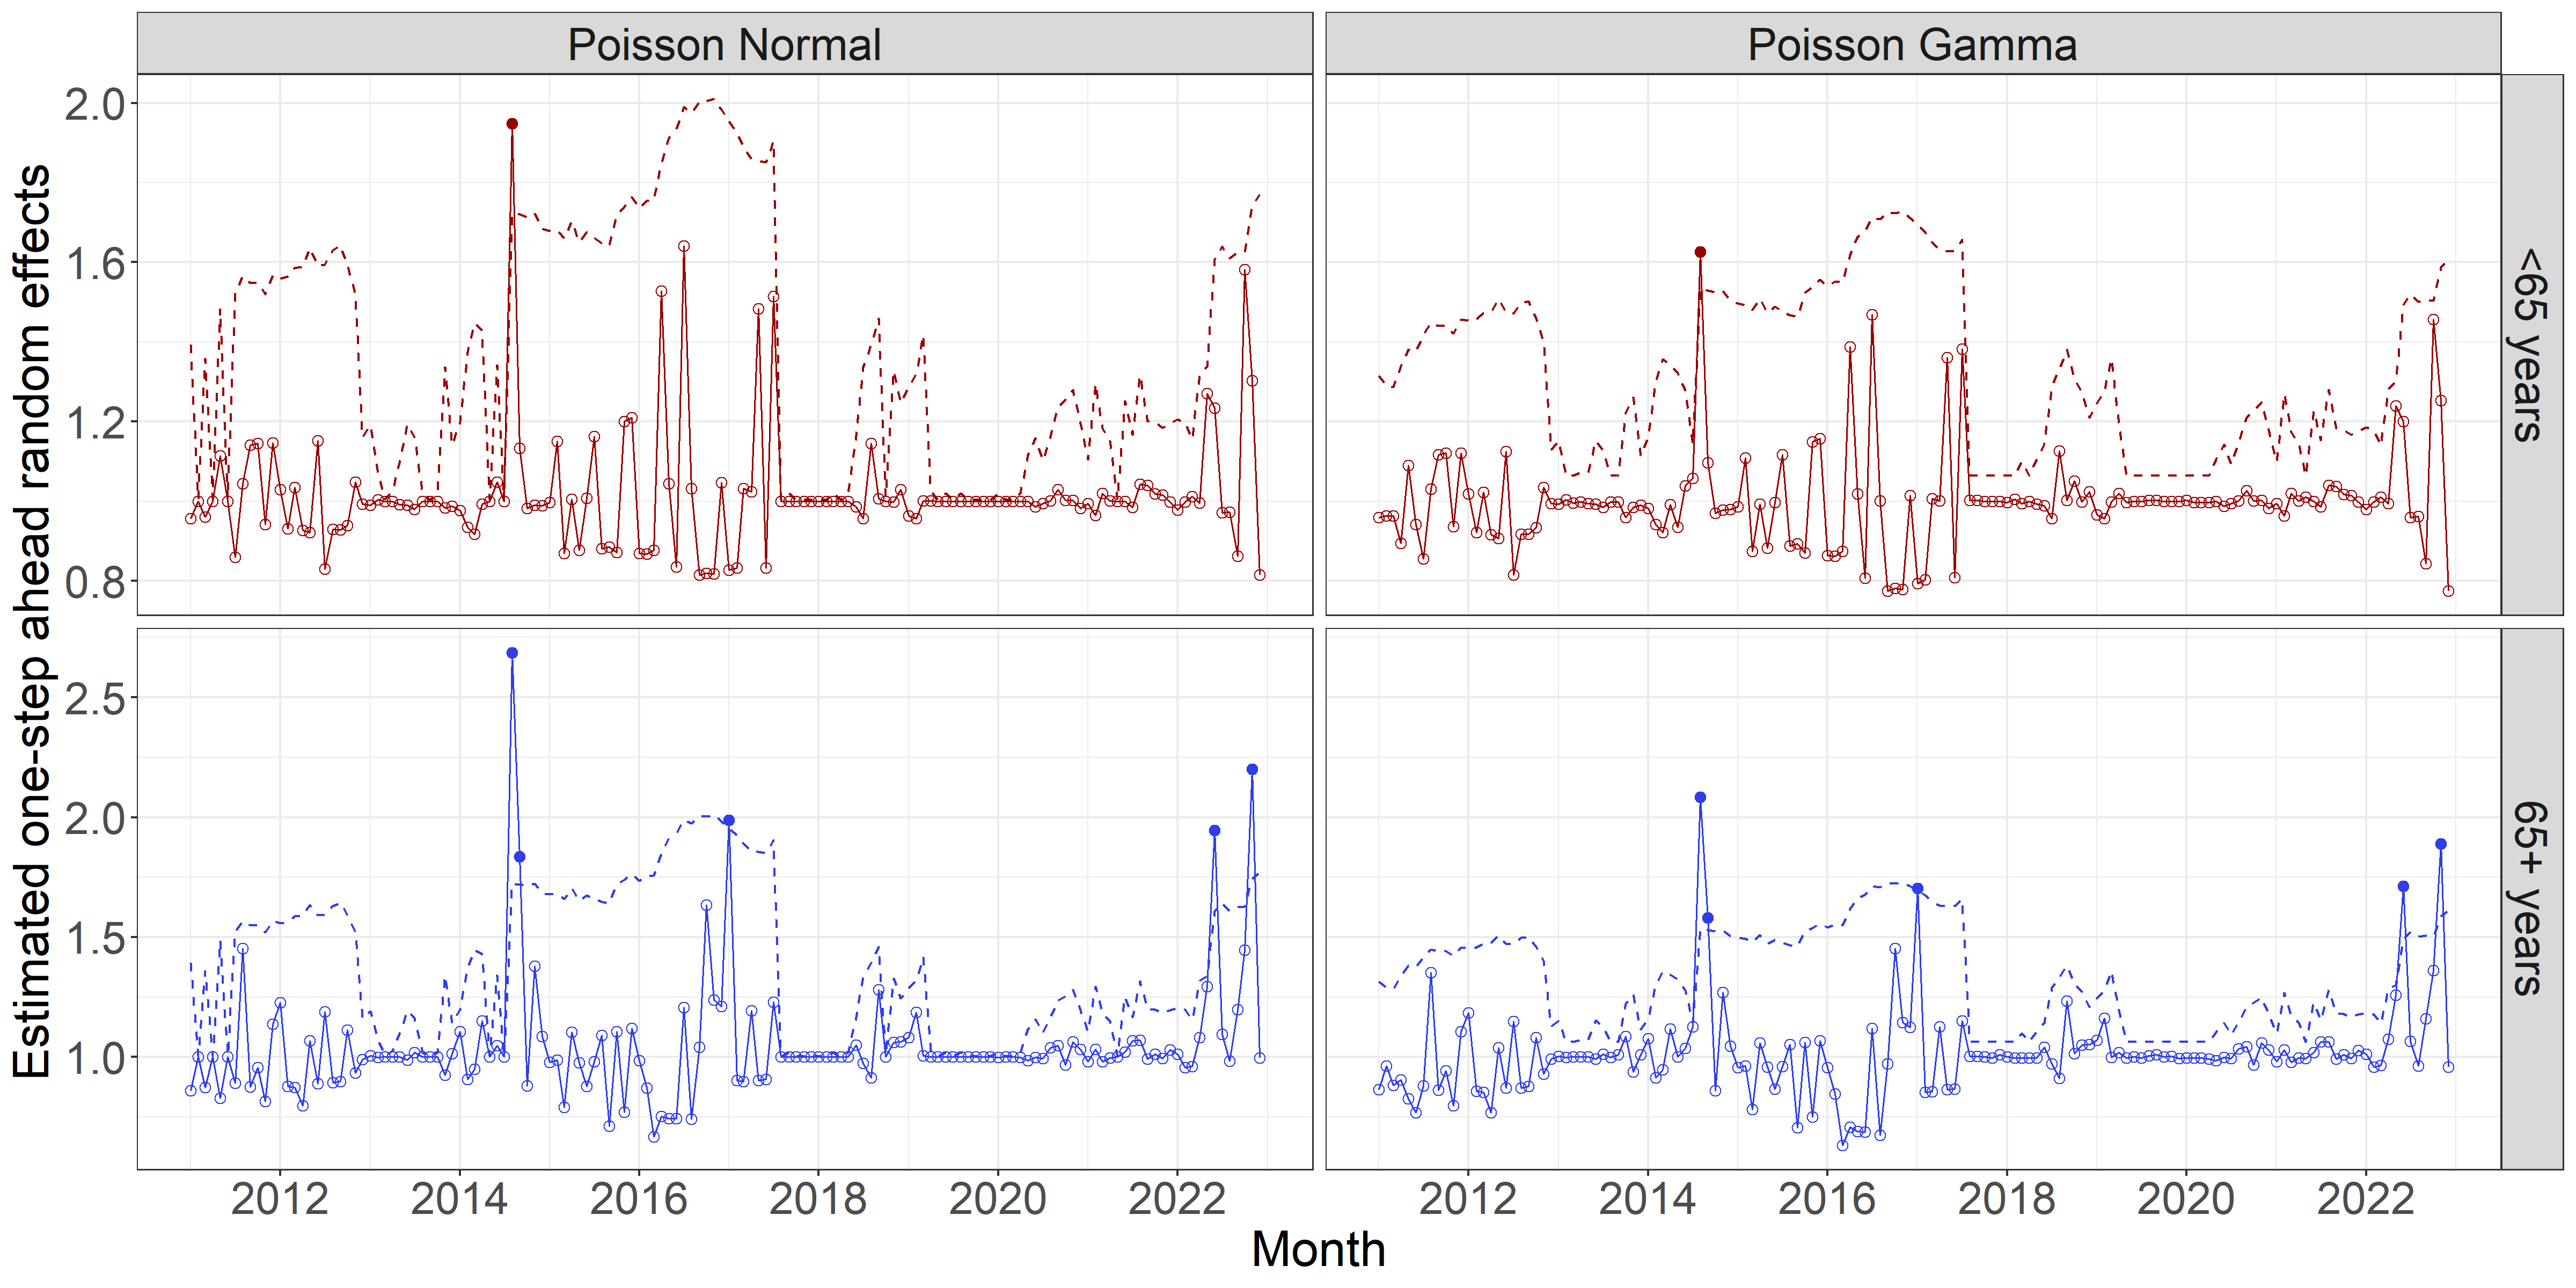
\includegraphics[width=1\linewidth]{../figures/Compare_novel_LIST} \caption{One-step ahead random effects \(u_{t_1}\) of \textit{Listeriosis} in Denmark, 2011-2022, as circles. Poisson Normal model (top) and Poisson Gamma model (bottom) monitor the disease. Alarm raised (solid circle) if \(u_{t_1}\) exceeds the threshold (dashed line).}\label{fig:CompareNovelLIST}
\end{figure}

\section{\textit{Shiggellosis}}

The data set utilized in this case study comprises monthly counts of Danish shigella cases, denoted as \(y_{it}\). The subscript \(i\) distinguishes between two age groups, with \(i = 1\) representing the age group below 25 years and \(i = 2\) representing the age group above 25 years. The subscript \(t\) represents the time period, ranging from \(t = 1,\cdots, T\), where \(T = 180\) corresponds to the total number of months starting in 2008.

Both the state-of-the-art outbreak detection algorithm and the novel outbreak detection algorithm are applied to this data set.

\subsection{Applying the state-of-the-art outbreak detection algorithm to \textit{Shigellosis}}



\begin{figure}[H]
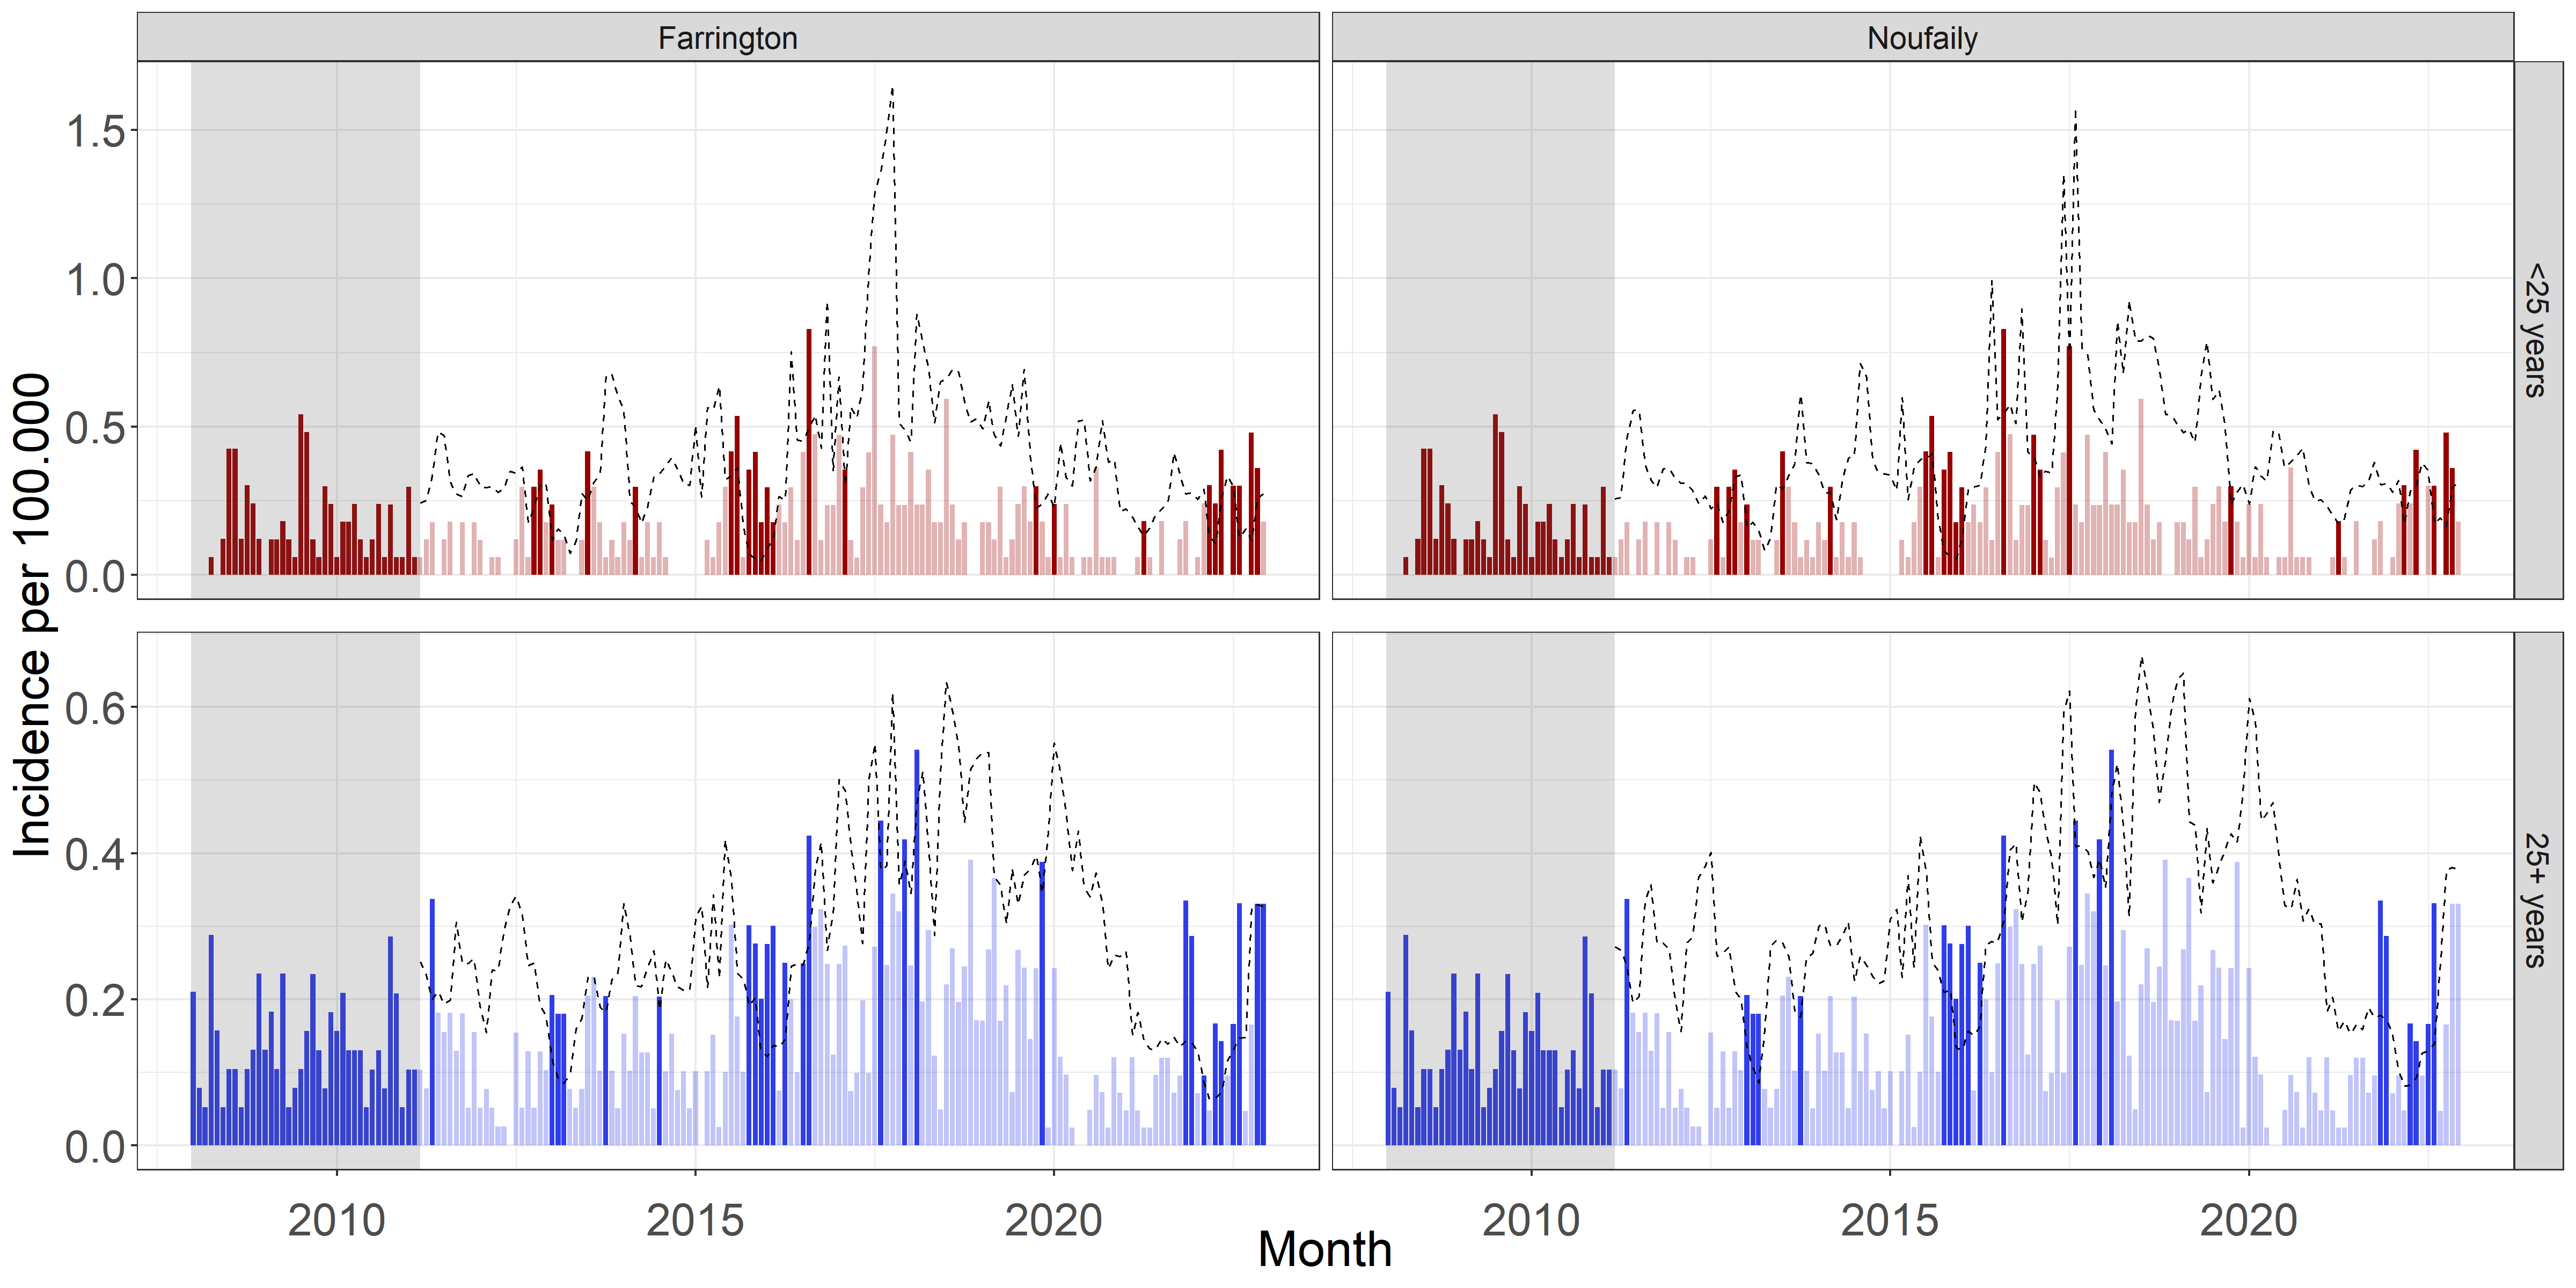
\includegraphics[width=1\linewidth]{../figures/Compare_stateOfTheArt_SHIG} \caption{Monthly \textit{Shigellosis} incidence per 100.000 in Denmark, 2008-2022. Monitored by (left) Farrington and (right) Noufaily method. Reference data for the estimation of model parameters from January 2008 to March 2011 (grey area). Threshold (dashed line) is computed for observations timepoints outside reference data. Alarm triggered (full opacity) if observations exceeds threshold.}\label{fig:CompareStateOfTheArtSHIG}
\end{figure}

\subsection{Applying the novel outbreak detection algorithm to \textit{Shigellosis}}



\begin{figure}[H]
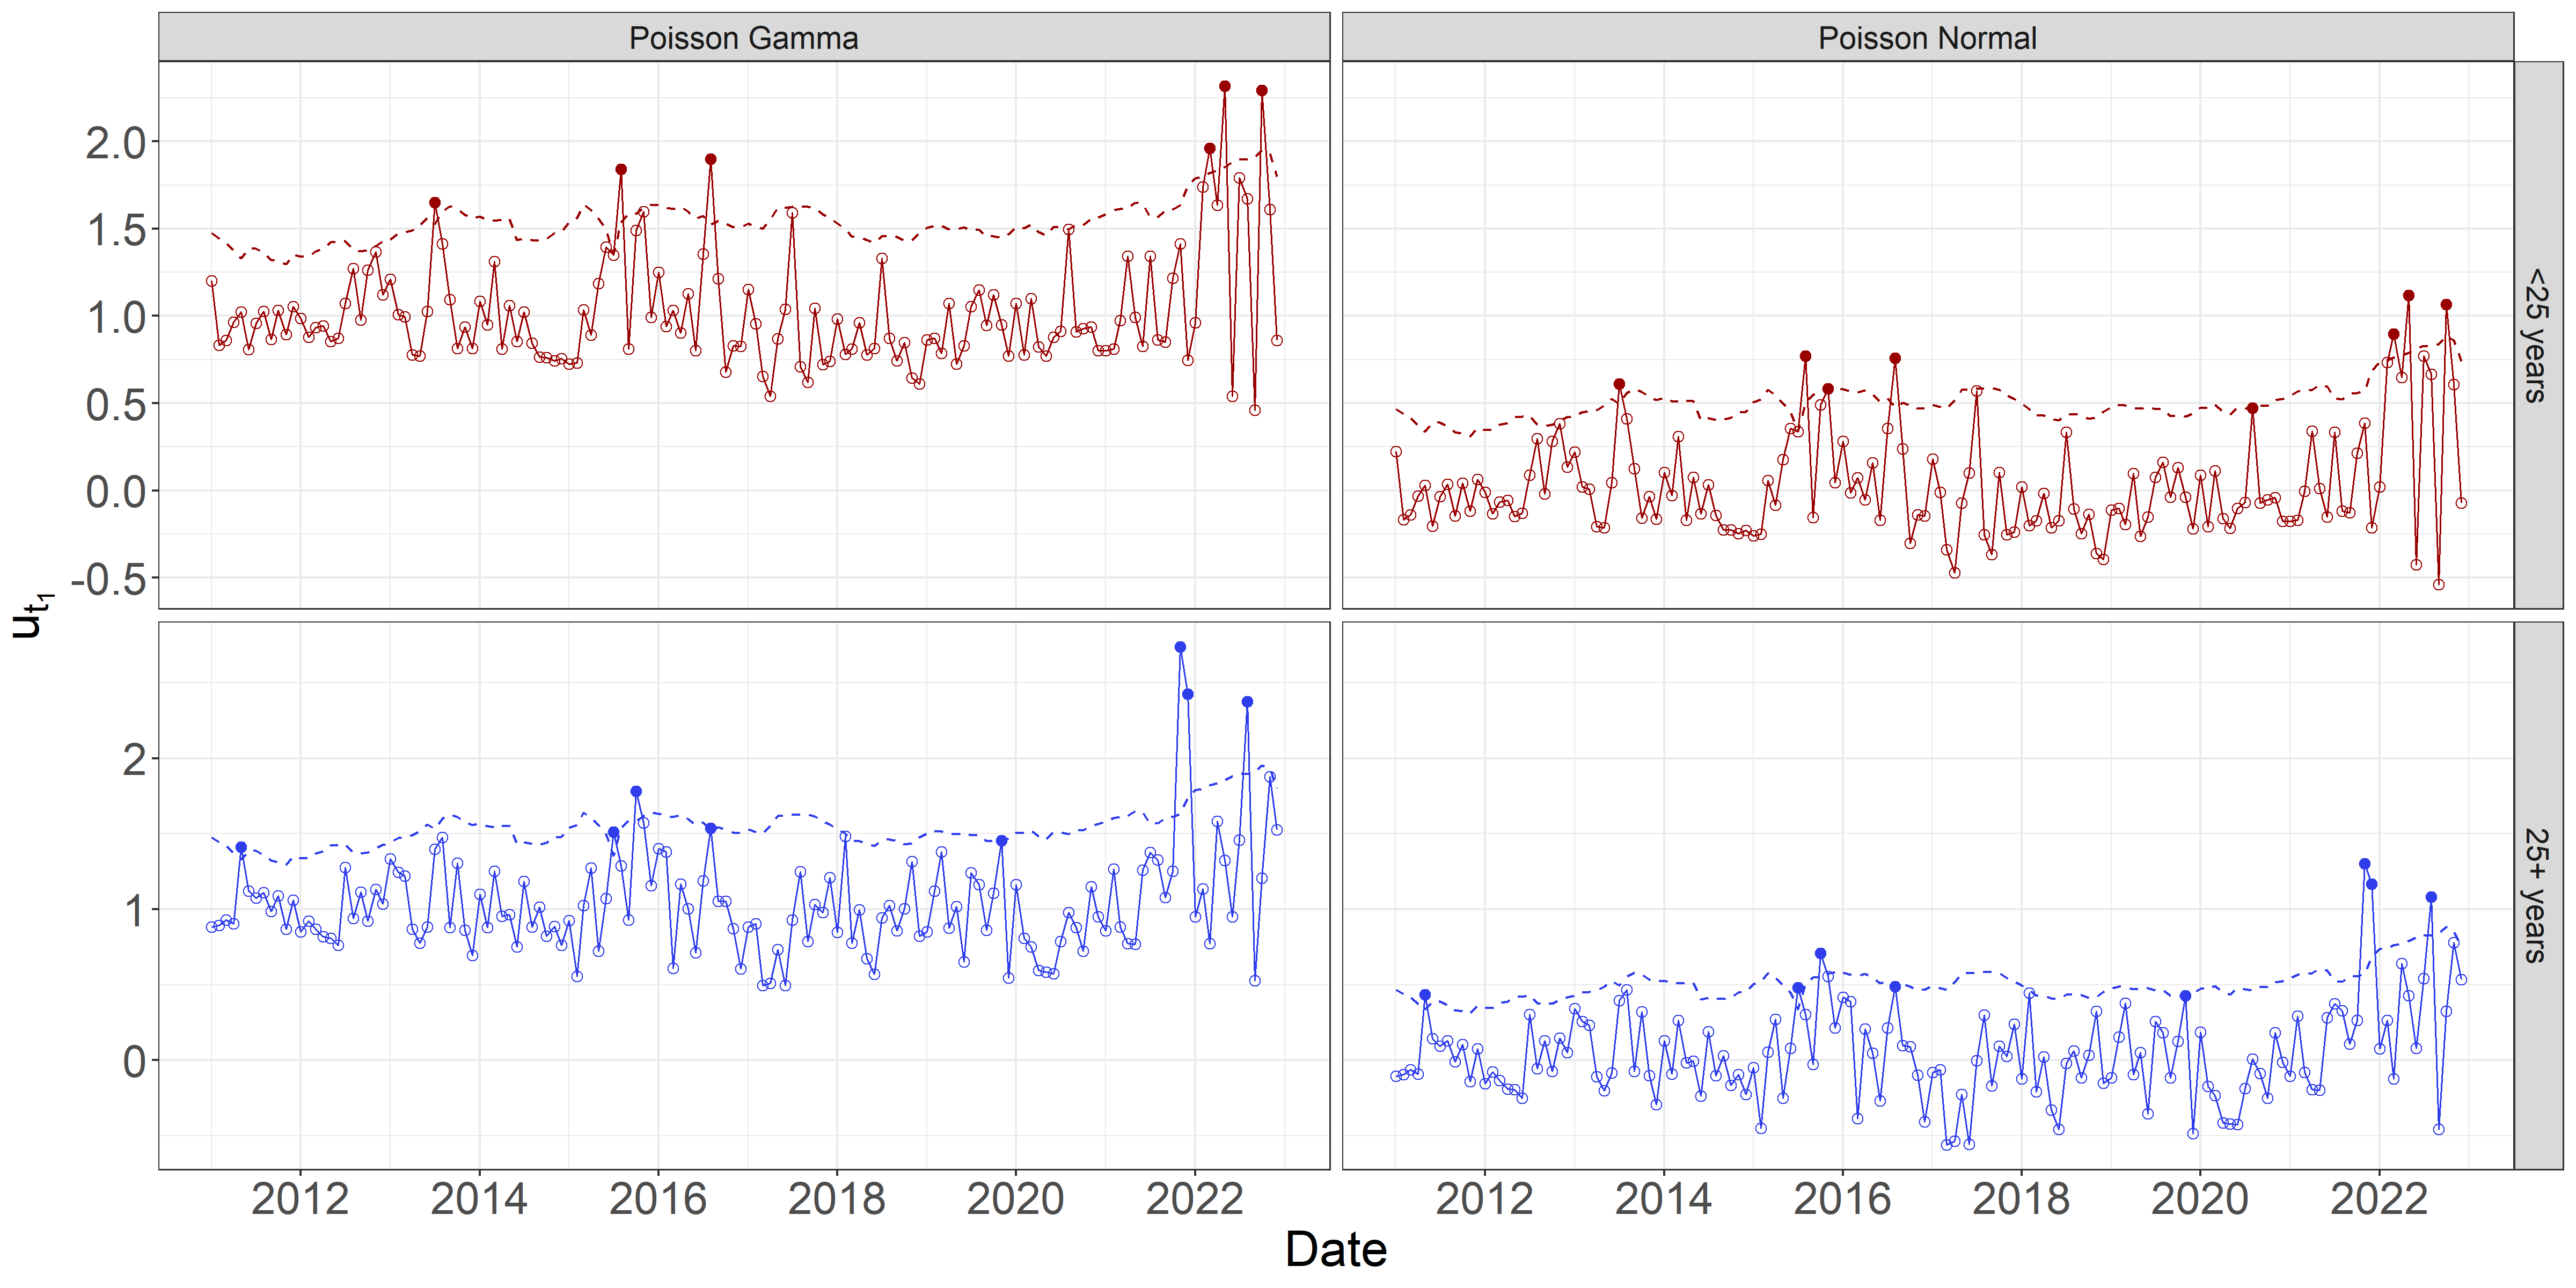
\includegraphics[width=1\linewidth]{../figures/Compare_novel_SHIG} \caption{One-step ahead random effects \(u_{t_1}\) of \textit{Shigellosis} in Denmark, 2011-2022, as circles. Poisson Normal model (top) and Poisson Gamma model (bottom) monitor the disease. Alarm raised (solid circle) if \(u_{t_1}\) exceeds the threshold (dashed line).}\label{fig:CompareNovelSHIG}
\end{figure}

\section{\textit{Salmonellosis}}

The data set utilized in this case study comprises monthly counts of Danish salmonella cases, denoted as \(y_{it}\). The subscript \(i\) differentiates between the six age groups \(i=1,\dots,6\). The subscript \(t\) represents the time period, ranging from \(t = 1,\cdots, T\), where \(T = 180\) corresponds to the total number of months starting in 2008.

Both the state-of-the-art outbreak detection algorithm and the novel outbreak detection algorithm are applied to this data set.

\subsection{Applying the state-of-the-art outbreak detection algorithm to \textit{Salmonellosis}}



\begin{figure}[H]
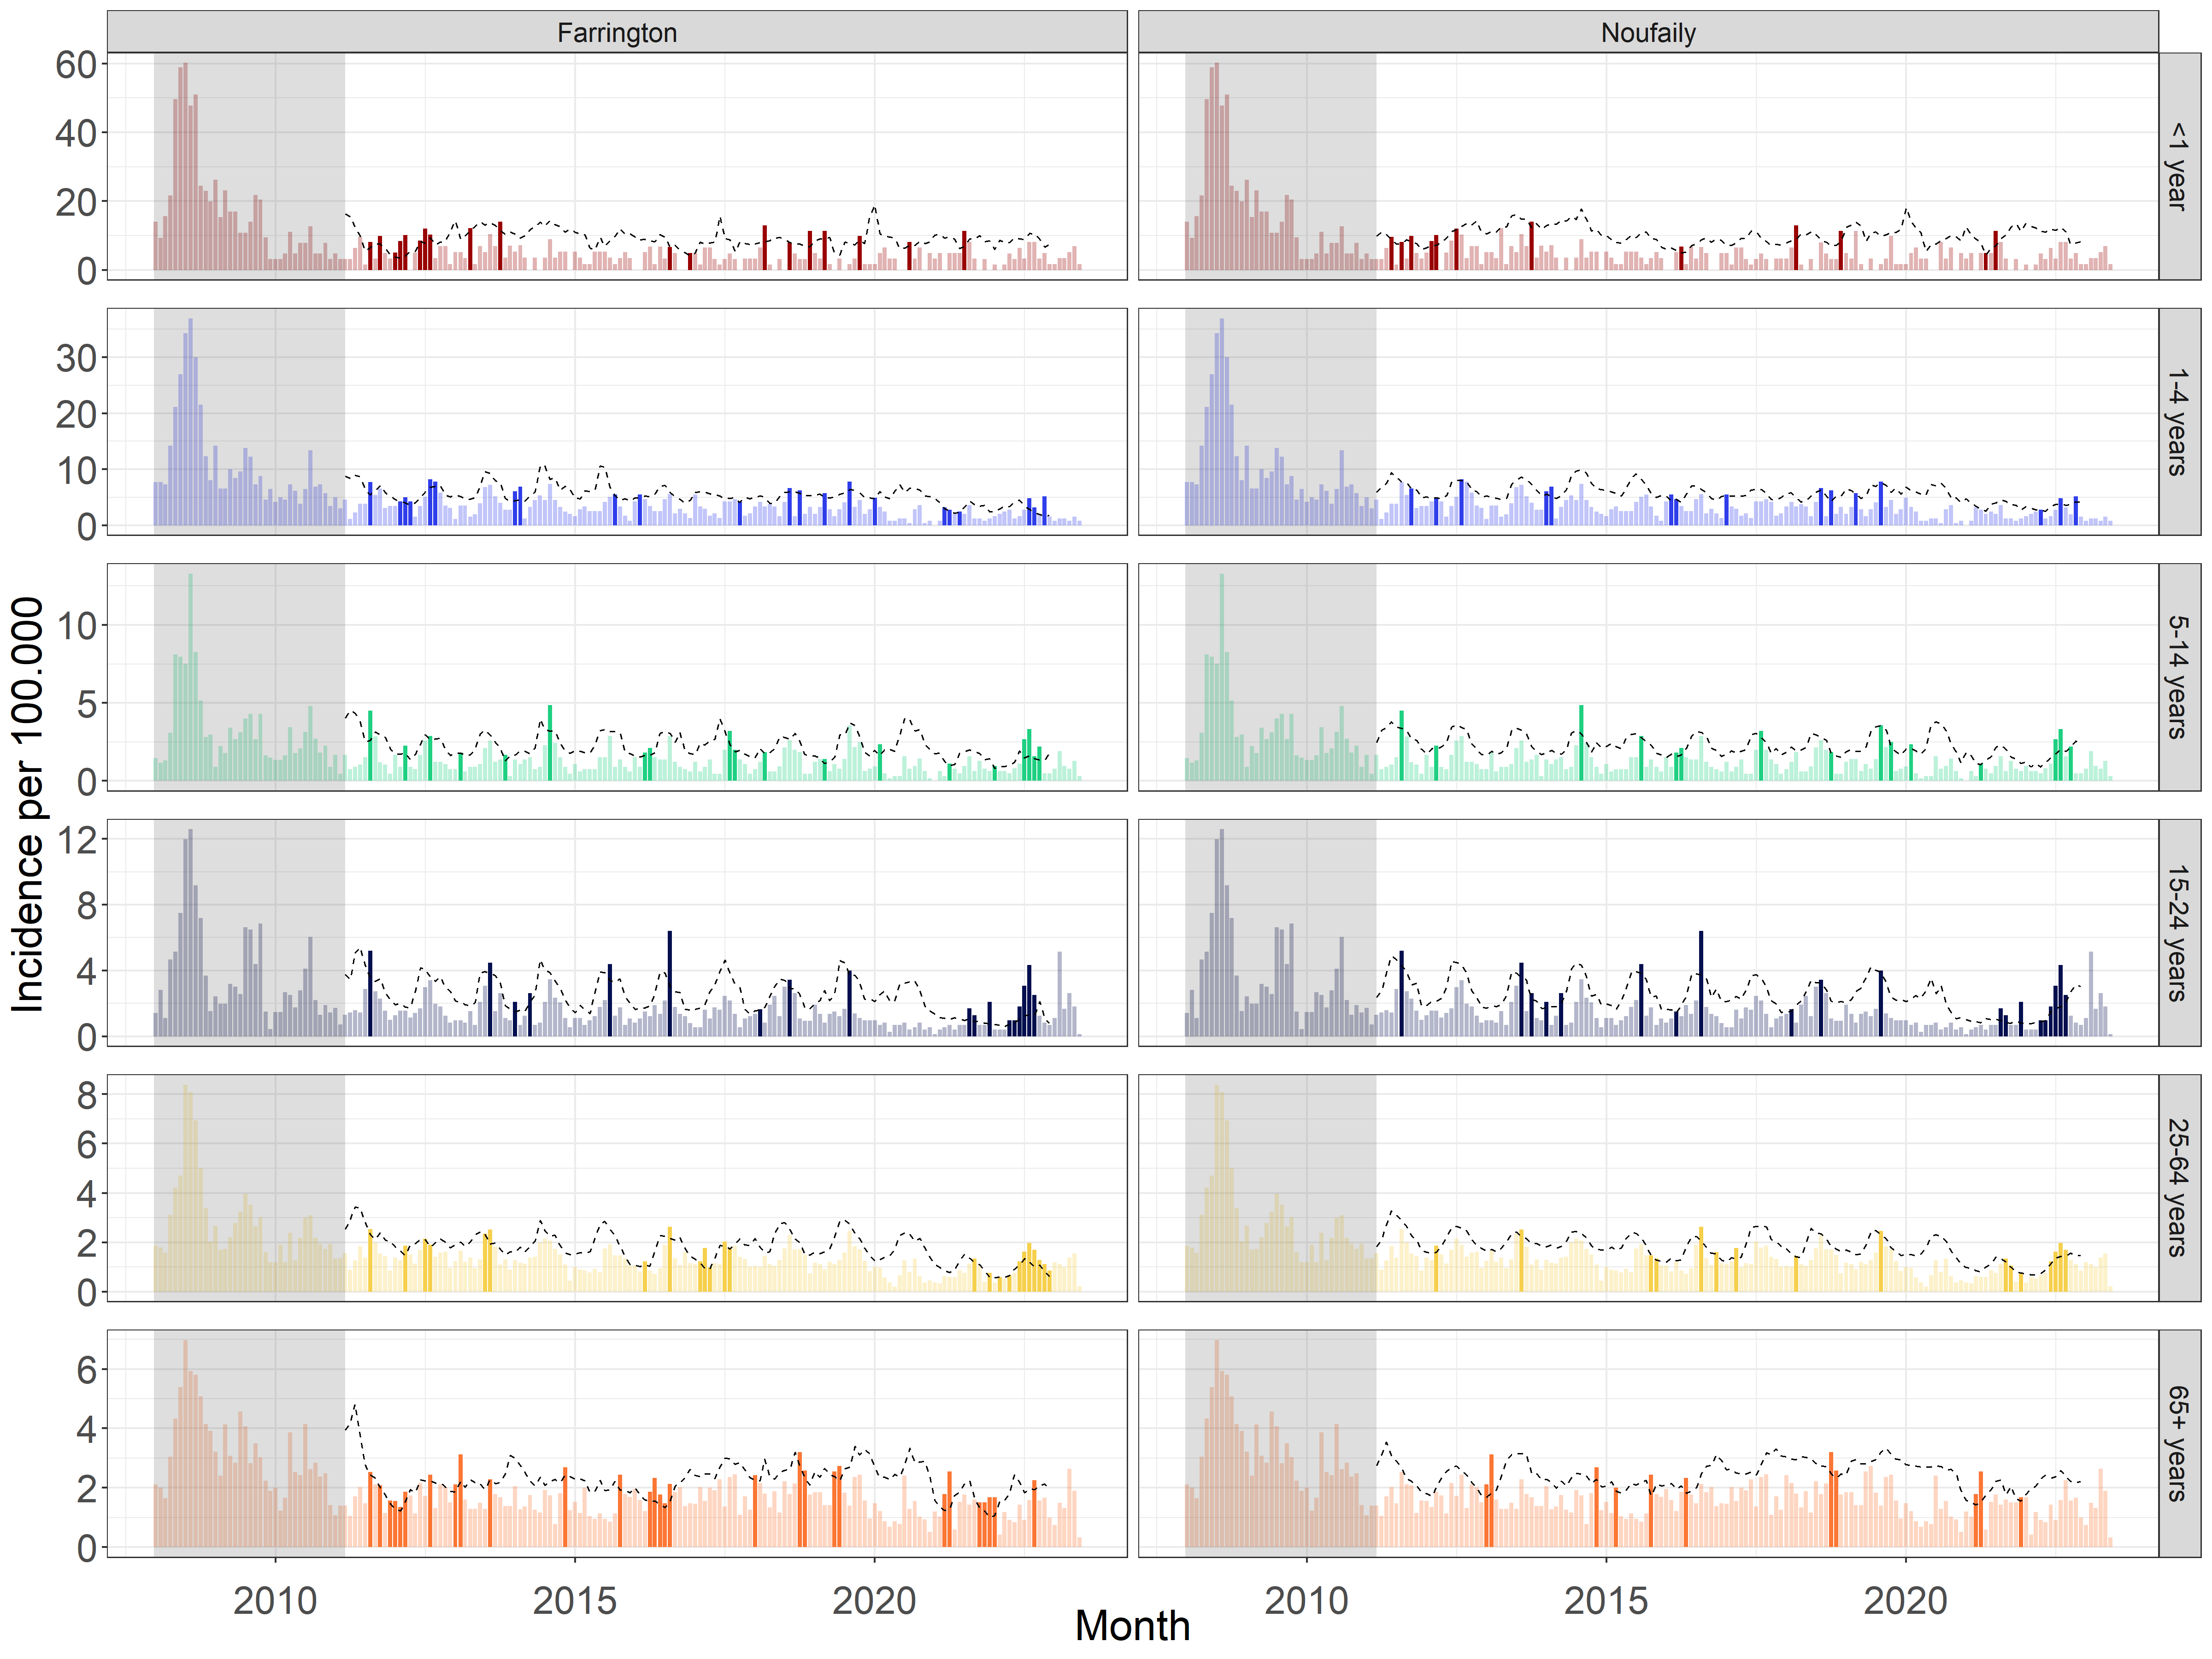
\includegraphics[width=1\linewidth]{../figures/Compare_stateOfTheArt_SALM} \caption{Monthly \textit{Salmonellosis} incidence per 100.000 in Denmark, 2008-2022. Monitored by (left) Farrington and (right) Noufaily method. Reference data for the estimation of model parameters from January 2008 to March 2011 (grey area). Threshold (dashed line) is computed for observations timepoints outside reference data. Alarm triggered (full opacity) if observations exceeds threshold.}\label{fig:CompareStateOfTheArtSALM}
\end{figure}

\subsection{Applying the novel outbreak detection algorithm to \textit{Salmonellosis}}



\begin{figure}[H]
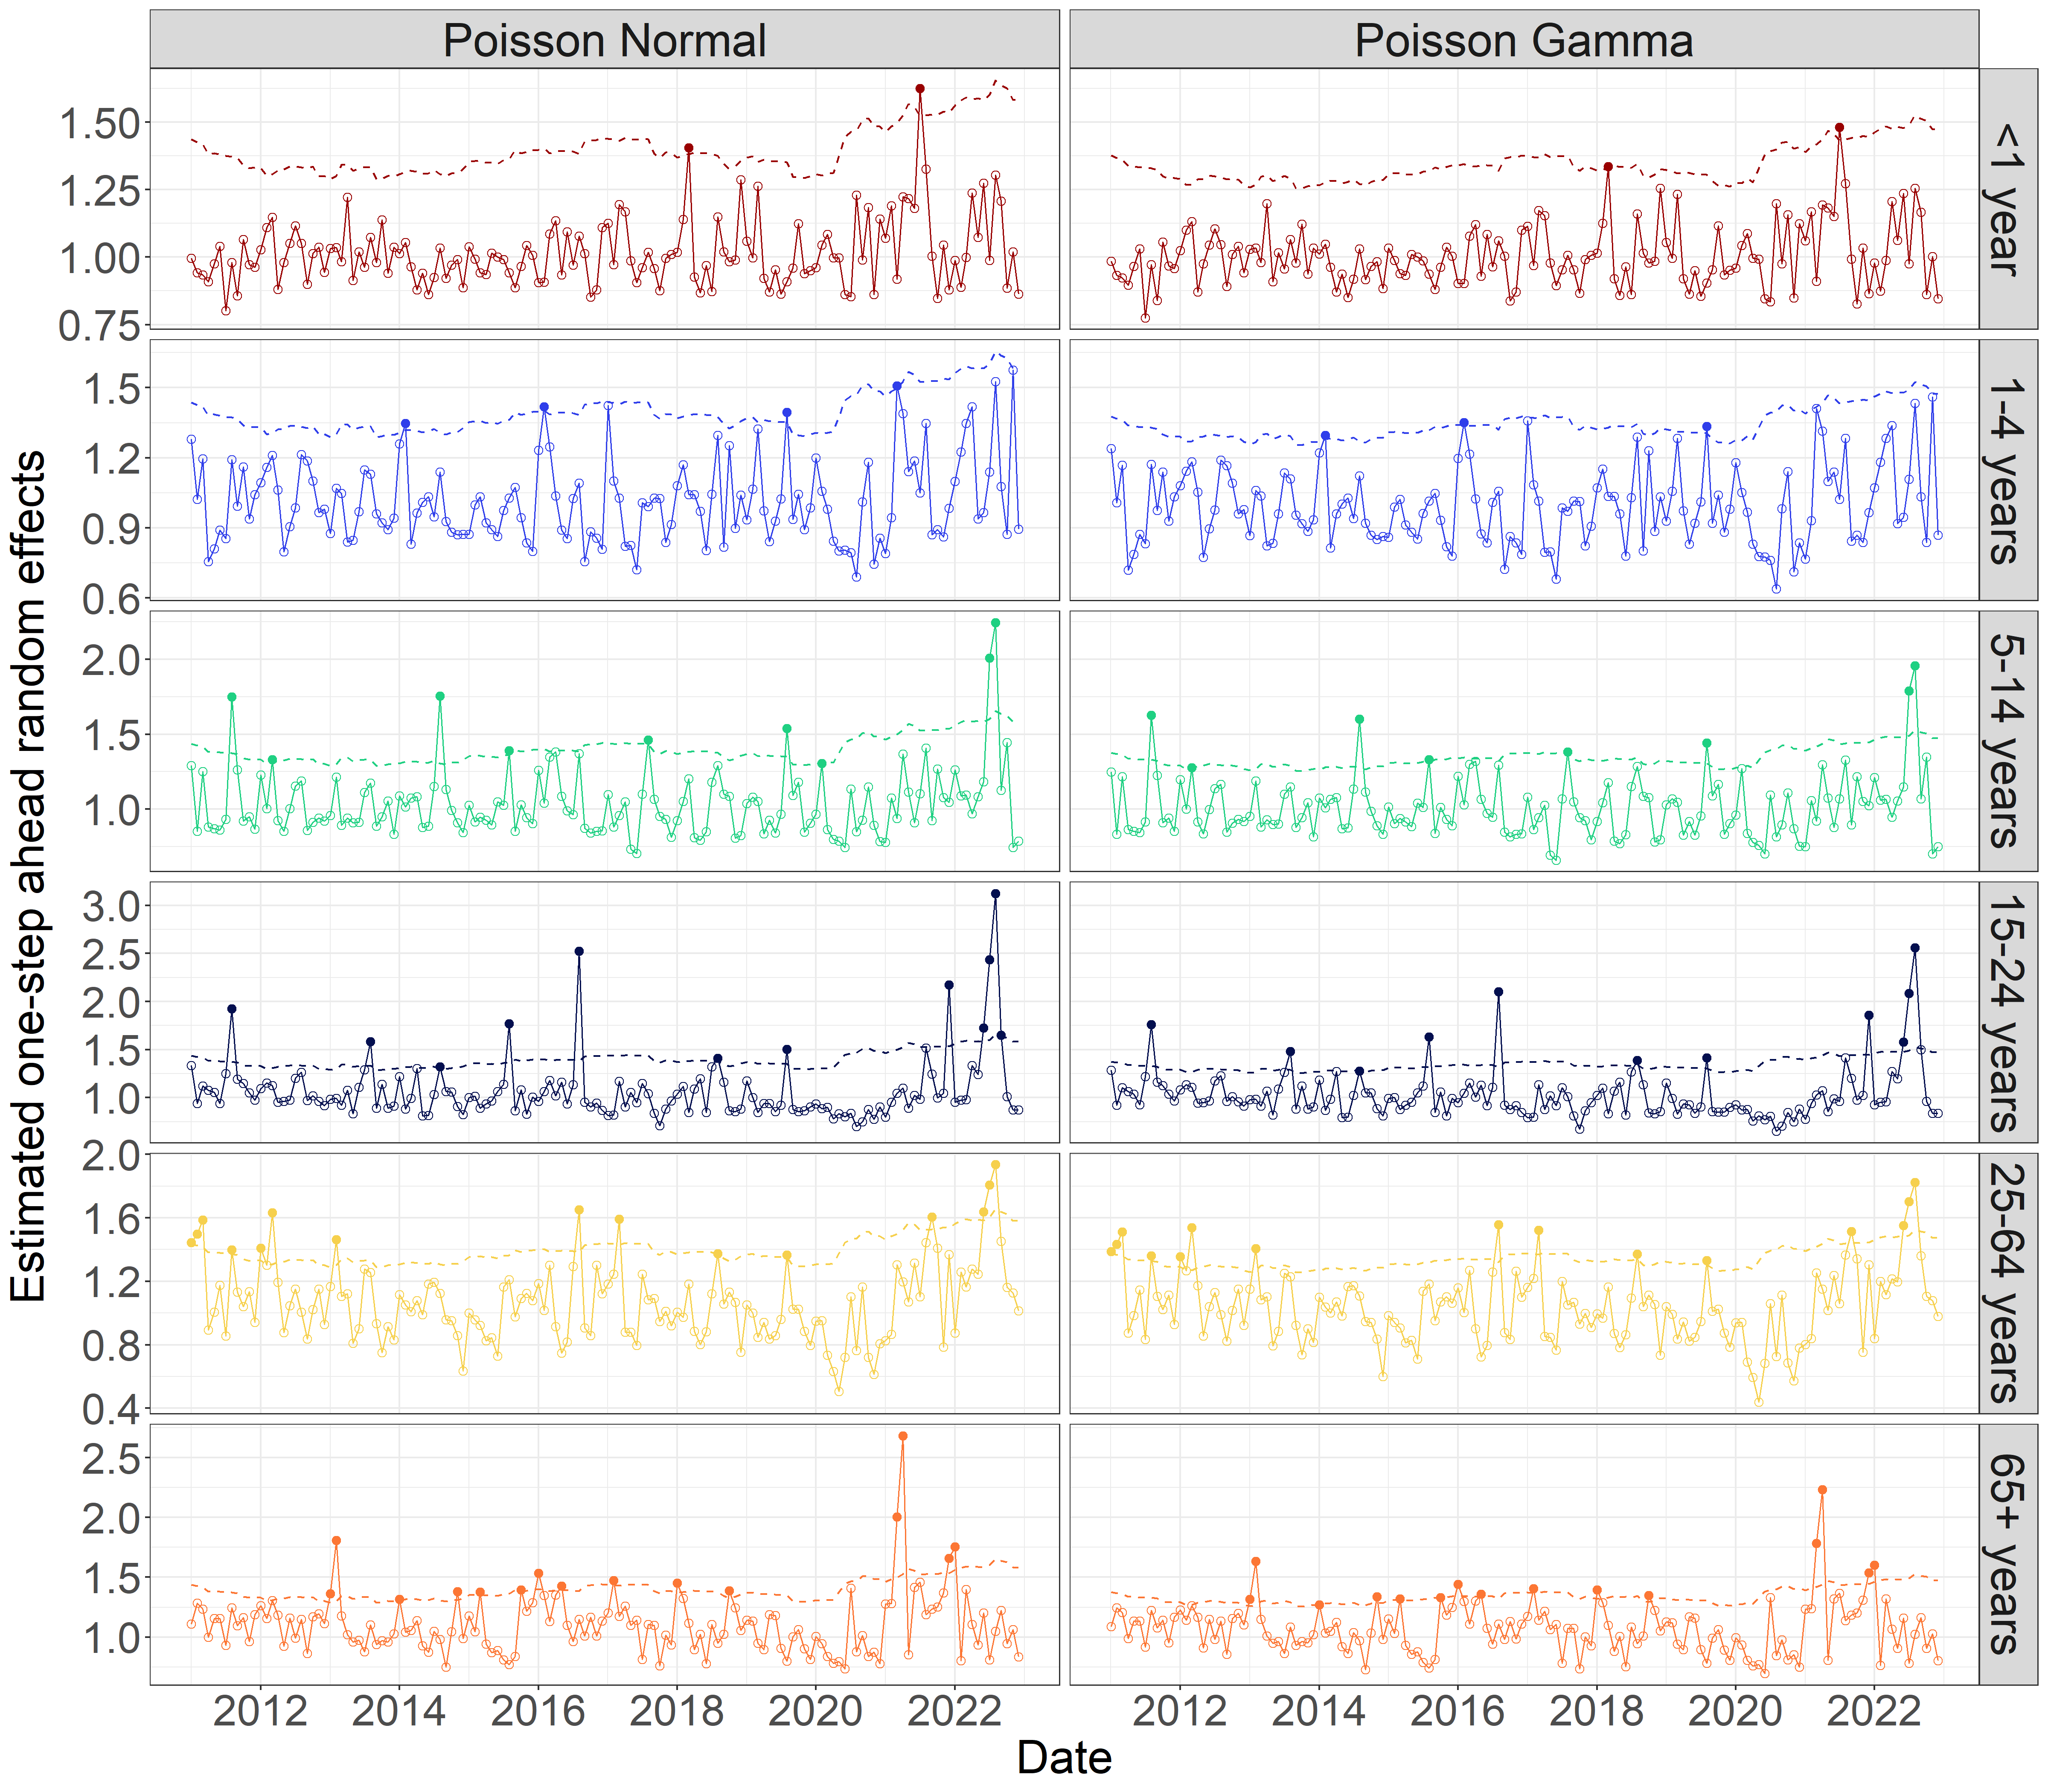
\includegraphics[width=1\linewidth]{../figures/Compare_novel_SALM} \caption{(ref:ref:CompareNovelSALM)}(\#fig:ref:CompareNovelSALM)
\end{figure}

\section{Performance comparison of novel methods}



\begin{figure}[H]
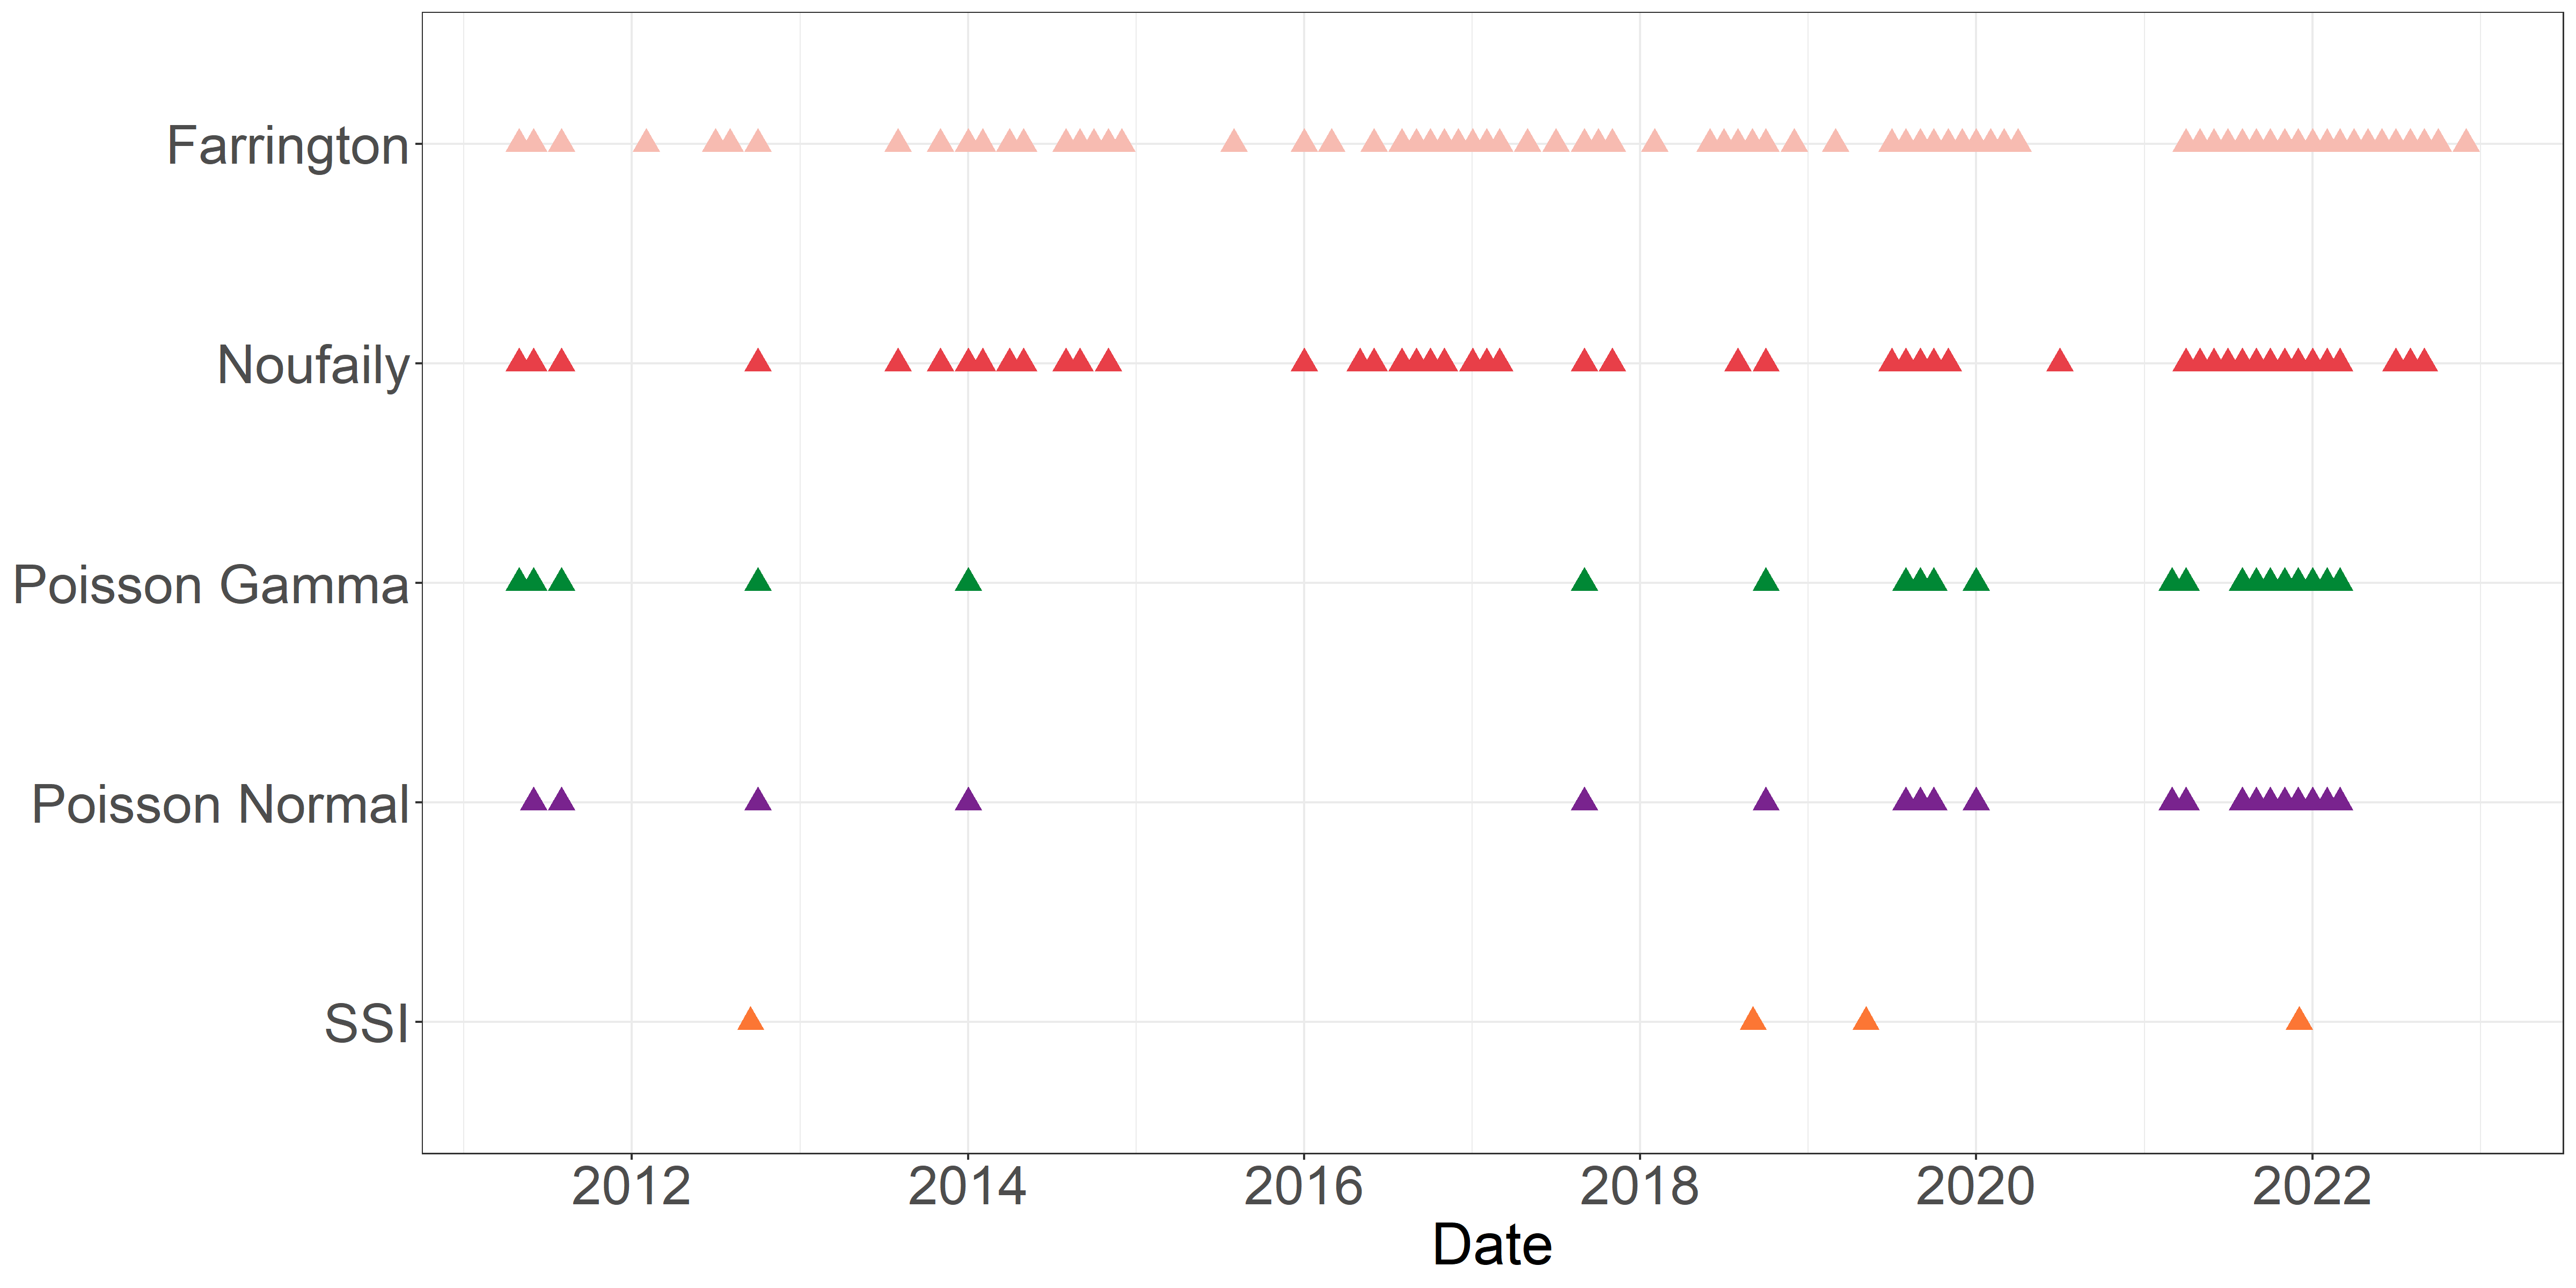
\includegraphics[width=1\linewidth]{../figures/Compare_alarms_STEC} \caption{Placeholder caption}\label{fig:CompareAlarmsSTEC}
\end{figure}



\begin{figure}[H]
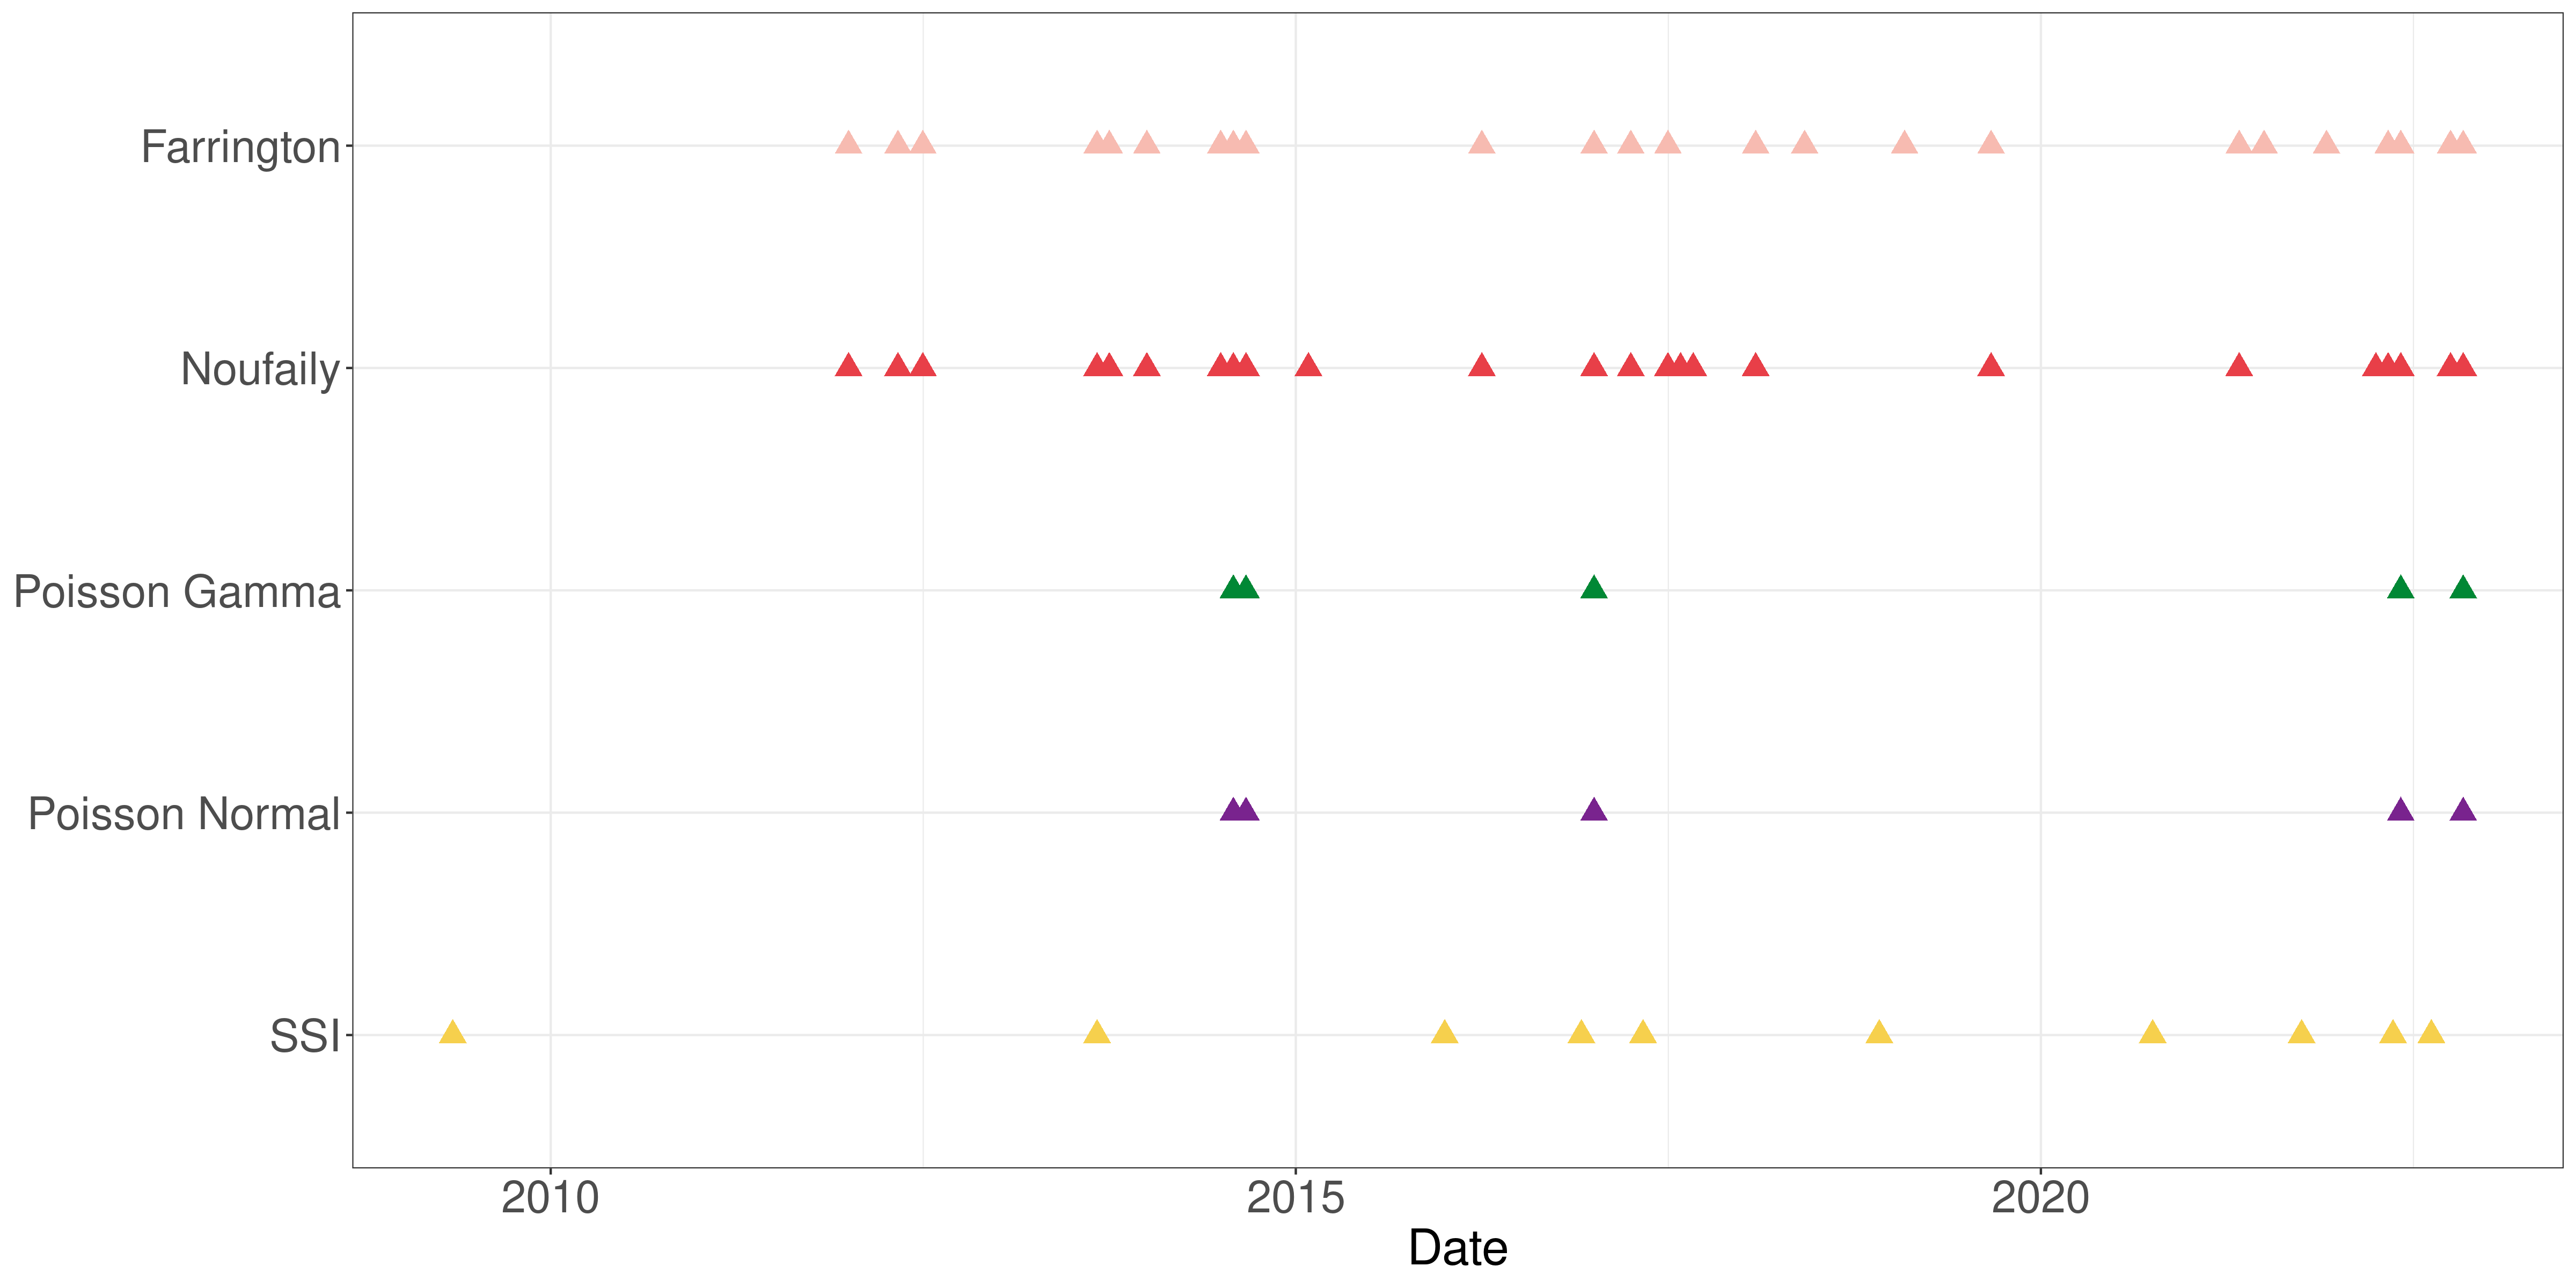
\includegraphics[width=1\linewidth]{../figures/Compare_alarms_LIST} \caption{Placeholder caption}\label{fig:CompareAlarmsLIST}
\end{figure}



\begin{figure}[H]
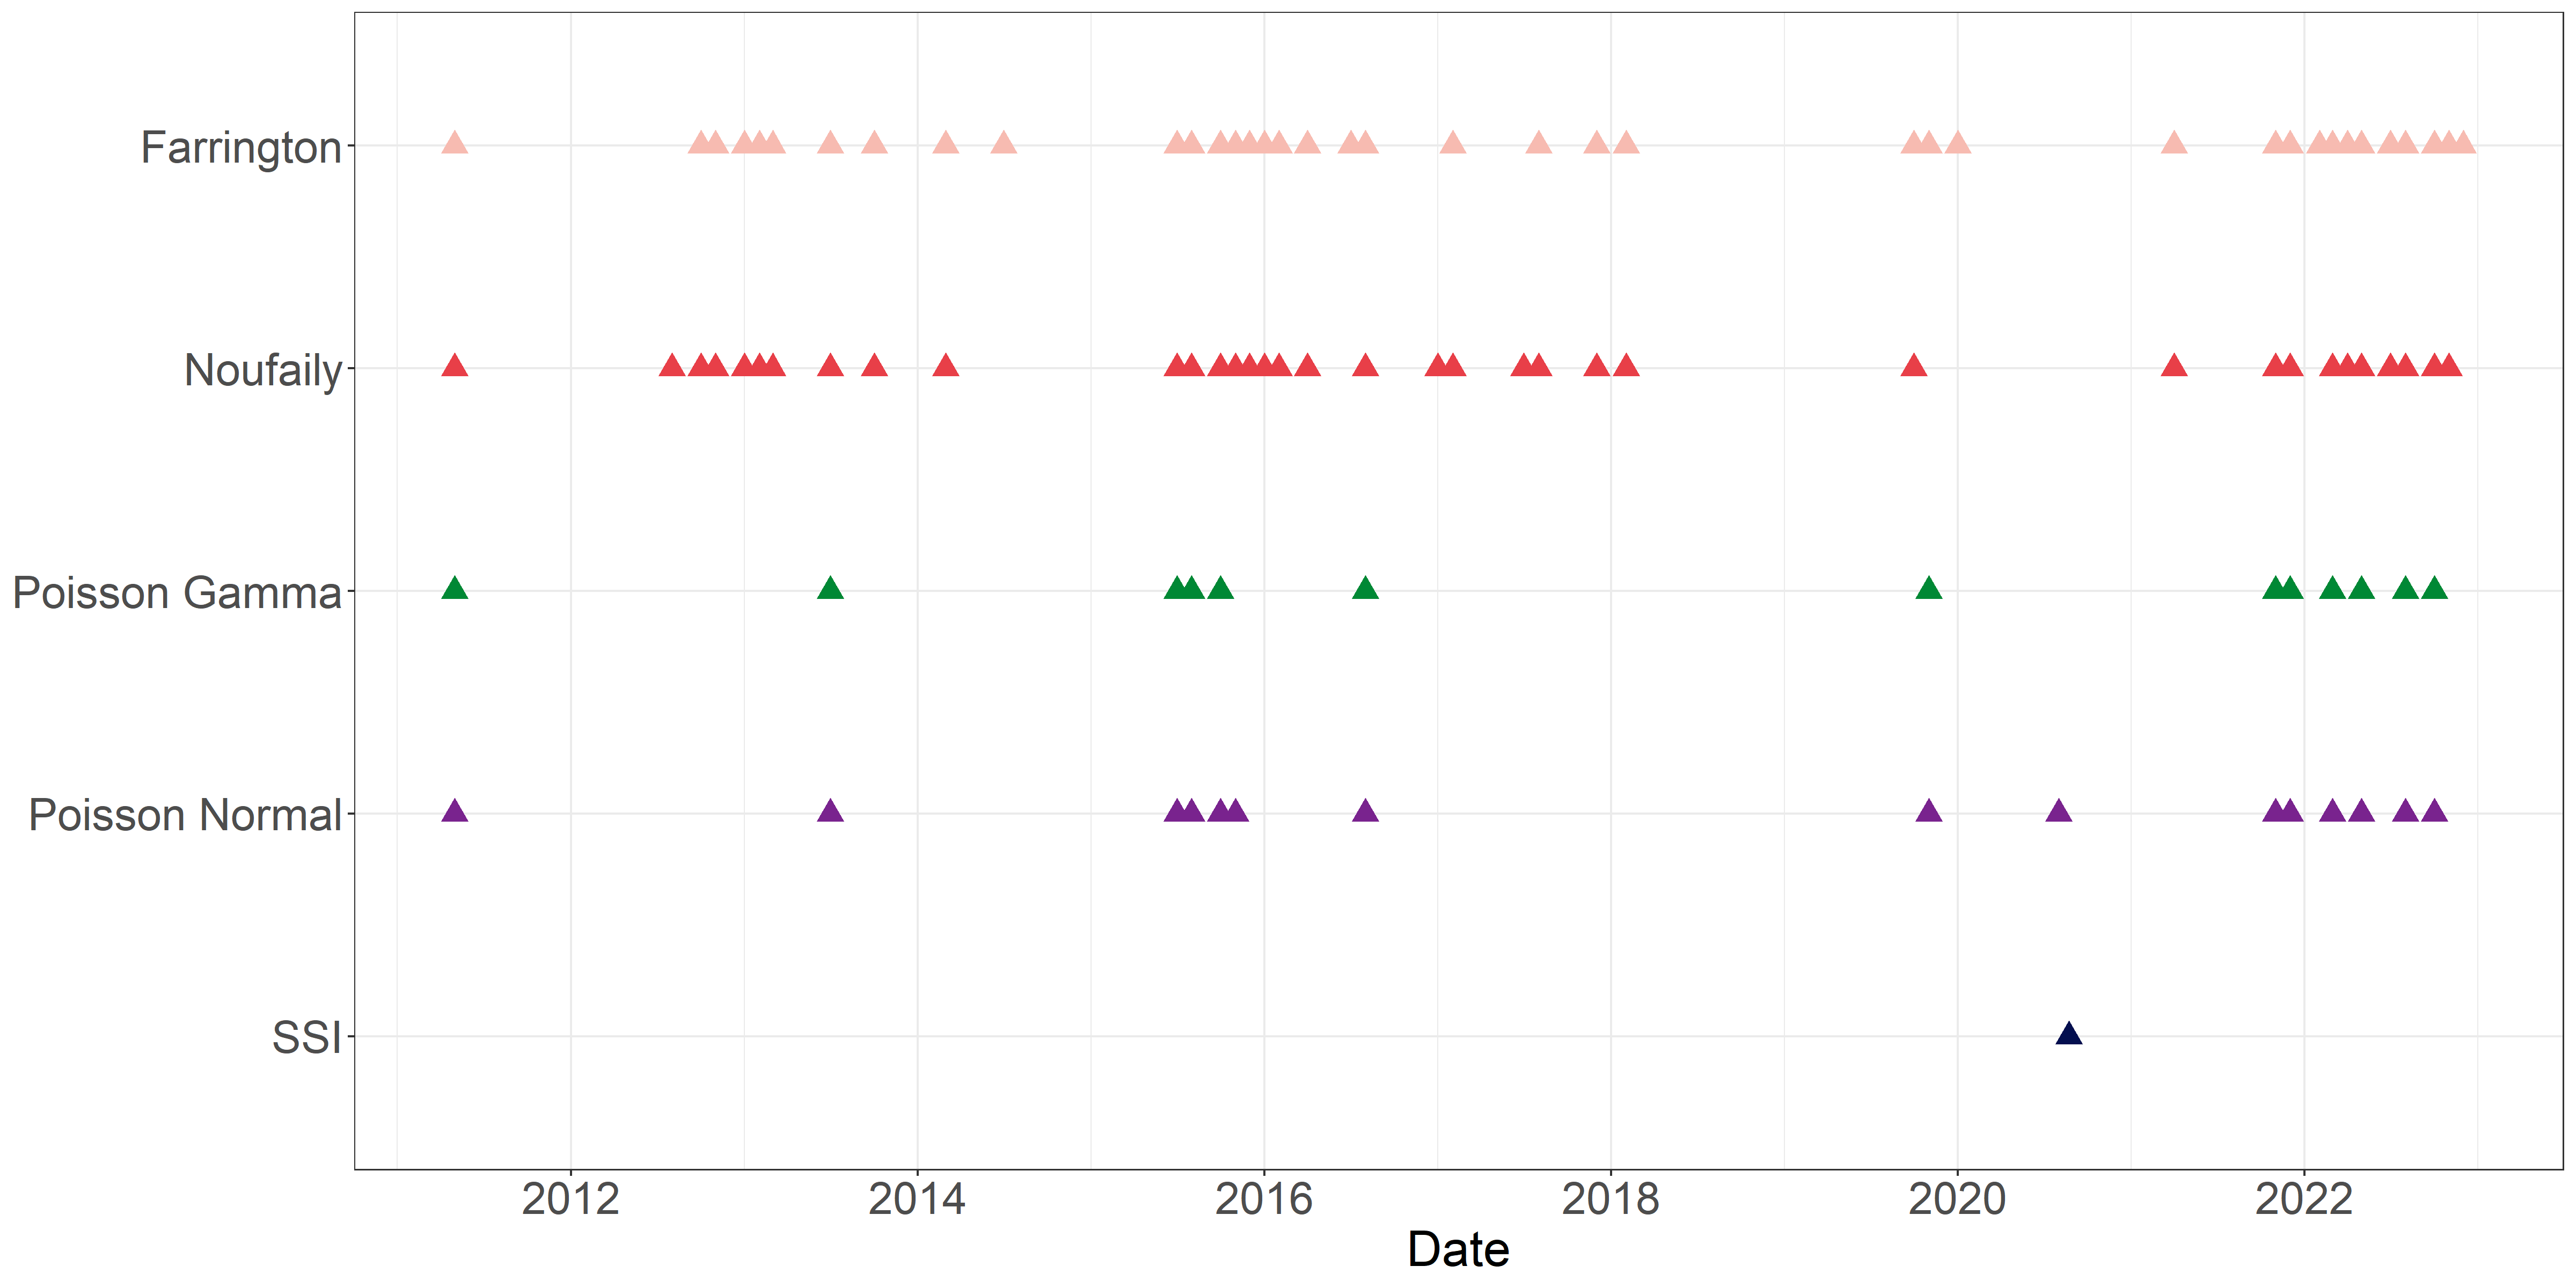
\includegraphics[width=1\linewidth]{../figures/Compare_alarms_SHIG} \caption{Placeholder caption}\label{fig:CompareAlarmsSHIG}
\end{figure}



\begin{figure}[H]
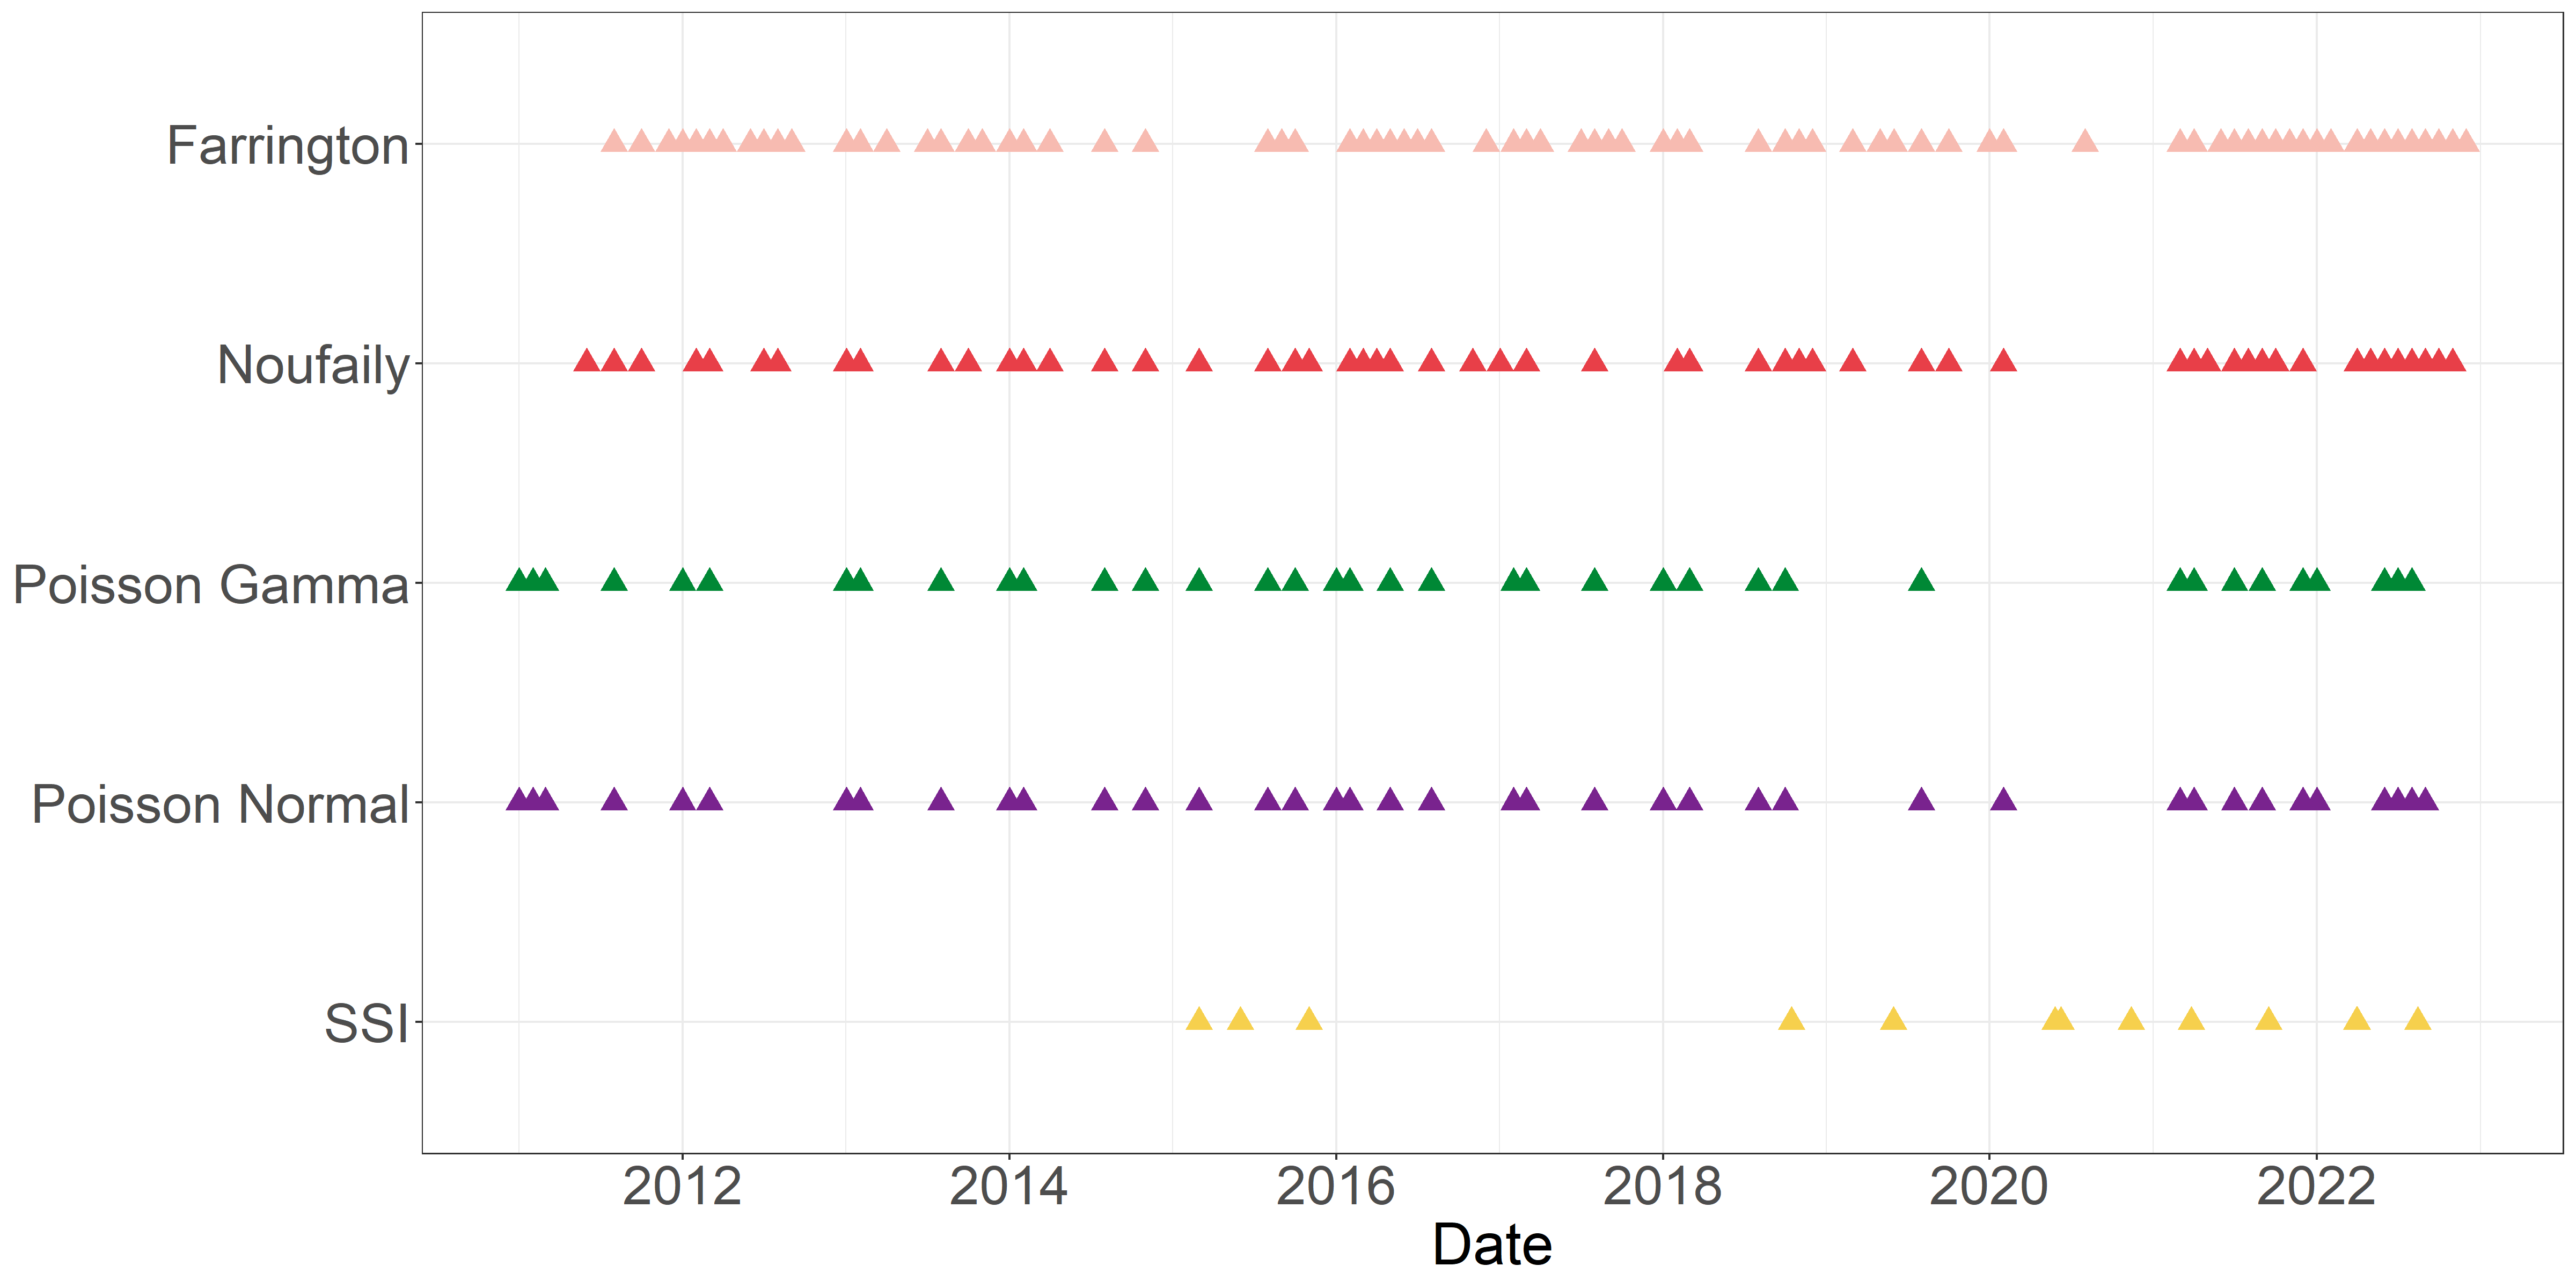
\includegraphics[width=1\linewidth]{../figures/Compare_alarms_SALM} \caption{Placeholder caption}\label{fig:CompareAlarmsSALM}
\end{figure}

\cleardoublepage

\chapter{Simulation study}

\blindtext

\blindtext

\cleardoublepage

\chapter{Discussion}

\blindtext

In the future, the utilization of MiBa-based surveillance has immense potential for disease surveillance. It has already demonstrated its value in various surveillance systems, such as the Healthcare-Associated Infections Database (HAIBA) for monitoring hospital-acquired infections and the COVID-19 surveillance system.

HAIBA, launched in 2015, was the first fully automated surveillance system built on MiBa data. It provides monitoring capabilities for hospital-acquired infections, enabling healthcare professionals to track and manage these infections more effectively. Similarly, the COVID-19 surveillance system, developed during 2020 and 2021, utilizes MiBa data to monitor and respond to the COVID-19 pandemic.

In addition to these systems, MiBa-based surveillance includes monitoring respiratory infections (such as influenza, pertussis, Mycoplasma pneumonia, and respiratory syncytial virus) and sexually transmitted diseases like chlamydia. While these surveillance systems currently have partial automation in data processing, there are plans to fully automate them in the near future.

Expanding on the field of automated disease outbreak detection is crucial to fully harness the potential of MiBa. By developing advanced algorithms and methodologies, it becomes possible to automatically analyze MiBa data and detect disease outbreaks in a timely manner. This can lead to early identification of outbreaks, allowing for prompt interventions and preventive measures.

Further research and development in automated disease outbreak detection, specifically tailored to leverage MiBa data, can significantly enhance our ability to detect and respond to infectious disease outbreaks more proactively and efficiently. By maximizing the potential of MiBa-based surveillance and continuously improving automated detection methods, we can strengthen our overall disease surveillance efforts and better protect public health.

\cleardoublepage

\chapter{Conclusion}

\blindtext

\cleardoublepage

\printbibliography[heading=bibintoc,title={Bibliography}]
\cleardoublepage 
\appendix

\chapter{Some probability functions}

This chapter serves as a reference, specifying notation, properties, and moments related to the various distributions used in this master thesis.

\begin{table}[h!]
\centering
  \resizebox{\textwidth}{!}{\begin{tabular}{m{0.12\textwidth}m{0.2\textwidth}m{0.50\textwidth}m{0.09\textwidth}m{0.09\textwidth}}
    \toprule
    Name & Support & Density & $\E[Y]$ & $\V[Y]$ \\
    \midrule
    Poisson \newline $\Pois(\lambda)$ & $0, 1, 2,\dots$ \newline $\lambda \in \mathbb{R}_{+}$ & $\frac{\lambda^{y}}{y!}\exp(-\lambda)$ & $\lambda$ & $\lambda$ \\
    \midrule
    Gamma \newline $\G(\alpha,\beta)$ & $\mathbb{R_{+}}$ \newline $\alpha \in \mathbb{R}_{+}, \beta \in \mathbb{R}_{+}$ & $\frac{1}{\Gamma(\alpha)\beta}\Big(\frac{y}{\beta}\Big)^{\alpha-1}\exp(-y/\beta)$ & $\alpha\beta$ & $\alpha\beta^2$ \\
    \midrule
    Neg. Bin. \newline $\NB(r,p)$ & $0, 1, 2,\dots$ \newline $r\in\mathbb{R}_+, p \in]0,1]$ & $\begin{pmatrix} r+y-1 \\ y \end{pmatrix} p^r(1-p)^y$ & $\frac{r(1+p)}{p}$ & $\frac{r(1-p)}{p^2}$ \\
    \midrule
    Normal \newline $\N(\mu, \sigma^2)$ & $\mathbb{R}$ \newline $\mu\in\mathbb{R}, \sigma^2\in\mathbb{R}_+$ & $\frac{1}{\sigma\sqrt{2\pi}}\exp\Big(-\frac{(y-\mu)^2}{2\sigma^2}\Big)$ & $\mu$ & $\sigma^2$ \\
    \bottomrule
  \end{tabular}}
  \caption{Density, support, mean value, and variance for a number of distributions used in this master thesis.}
  \label{table:probabilityFunctions}
\end{table}

\chapter{C++ templates for the negative joint log-likelihood}\label{cpp}

This chapter presents the user templates for the hierarchical Poisson Normal model in \eqref{eq:PoisN} and the hierarachical Poisson Gamma model in \eqref{eq:PoisGam}.

The user template for the hierarchical Poisson Normal model specified in \eqref{eq:PoisN} is

\begin{Shaded}
\begin{Highlighting}[]
\PreprocessorTok{\#include }\ImportTok{\textless{}TMB.hpp\textgreater{}}
\KeywordTok{template}\OperatorTok{\textless{}}\KeywordTok{class}\NormalTok{ Type}\OperatorTok{\textgreater{}}
\NormalTok{Type objective\_function}\OperatorTok{\textless{}}\NormalTok{Type}\OperatorTok{\textgreater{}::}\KeywordTok{operator}\OperatorTok{()} \OperatorTok{()}
\OperatorTok{\{}
  \CommentTok{// R input data}
\NormalTok{  DATA\_VECTOR}\OperatorTok{(}\NormalTok{y}\OperatorTok{);}                               \CommentTok{// Count data}
\NormalTok{  DATA\_VECTOR}\OperatorTok{(}\NormalTok{x}\OperatorTok{);}                               \CommentTok{// Population size}
\NormalTok{  DATA\_MATRIX}\OperatorTok{(}\NormalTok{X}\OperatorTok{);}                               \CommentTok{// Design matrix}
\NormalTok{  PARAMETER\_VECTOR}\OperatorTok{(}\NormalTok{u}\OperatorTok{);}                          \CommentTok{// Random effects}
  \CommentTok{// Parameters}
\NormalTok{  PARAMETER\_VECTOR}\OperatorTok{(}\NormalTok{beta}\OperatorTok{);}                       \CommentTok{// Fixed effects parameters}
\NormalTok{  PARAMETER}\OperatorTok{(}\NormalTok{log\_sigma\_u}\OperatorTok{);}                       \CommentTok{// Model parameter}
\NormalTok{  vector}\OperatorTok{\textless{}}\NormalTok{Type}\OperatorTok{\textgreater{}}\NormalTok{ lambda  }\OperatorTok{=}\NormalTok{ exp}\OperatorTok{(}\NormalTok{X}\OperatorTok{*}\NormalTok{beta}\OperatorTok{{-}}\NormalTok{log}\OperatorTok{(}\NormalTok{x}\OperatorTok{)+}\NormalTok{u}\OperatorTok{);}  \CommentTok{// Construct \textquotesingle{}lambda\textquotesingle{}}
\NormalTok{  Type sigma\_u }\OperatorTok{=}\NormalTok{ exp}\OperatorTok{(}\NormalTok{log\_sigma\_u}\OperatorTok{);}              \CommentTok{// And the model parameters}
\NormalTok{  Type mean\_ran }\OperatorTok{=}\NormalTok{ Type}\OperatorTok{(}\DecValTok{0}\OperatorTok{);}
  \CommentTok{// Objective function}
\NormalTok{  Type f }\OperatorTok{=} \DecValTok{0}\OperatorTok{;}                                   \CommentTok{// Declare the objective}
\NormalTok{  f }\OperatorTok{{-}=}\NormalTok{ sum}\OperatorTok{(}\NormalTok{dnorm}\OperatorTok{(}\NormalTok{u}\OperatorTok{,}\NormalTok{mean\_ran}\OperatorTok{,}\NormalTok{sigma\_u}\OperatorTok{,}\KeywordTok{true}\OperatorTok{));}     \CommentTok{// Calculate the objective}
\NormalTok{  f }\OperatorTok{{-}=}\NormalTok{ sum}\OperatorTok{(}\NormalTok{dpois}\OperatorTok{(}\NormalTok{y}\OperatorTok{,}\NormalTok{lambda}\OperatorTok{,}\KeywordTok{true}\OperatorTok{));}               \CommentTok{// Calculate the objective}
  \ControlFlowTok{return}\NormalTok{ f}\OperatorTok{;}
\OperatorTok{\}}
\end{Highlighting}
\end{Shaded}

The user template for the hierarchical Poisson Gamma model specified in \eqref{eq:PoisGam} is

\begin{Shaded}
\begin{Highlighting}[]
\PreprocessorTok{\#include }\ImportTok{\textless{}TMB.hpp\textgreater{}}
\KeywordTok{template}\OperatorTok{\textless{}}\KeywordTok{class}\NormalTok{ Type}\OperatorTok{\textgreater{}}
\NormalTok{Type objective\_function}\OperatorTok{\textless{}}\NormalTok{Type}\OperatorTok{\textgreater{}::}\KeywordTok{operator}\OperatorTok{()} \OperatorTok{()}
\OperatorTok{\{}
  \CommentTok{// Data}
\NormalTok{  DATA\_VECTOR}\OperatorTok{(}\NormalTok{y}\OperatorTok{);}                             \CommentTok{// Count data}
\NormalTok{  DATA\_VECTOR}\OperatorTok{(}\NormalTok{x}\OperatorTok{);}                             \CommentTok{// Population size}
\NormalTok{  DATA\_MATRIX}\OperatorTok{(}\NormalTok{X}\OperatorTok{);}                             \CommentTok{// Design matrix}
  \CommentTok{// Parameters}
\NormalTok{  PARAMETER\_VECTOR}\OperatorTok{(}\NormalTok{beta}\OperatorTok{);}                     \CommentTok{// Fixed effects parameters}
\NormalTok{  PARAMETER}\OperatorTok{(}\NormalTok{log\_phi\_u}\OperatorTok{);}                       \CommentTok{// Model parameter}
\NormalTok{  vector}\OperatorTok{\textless{}}\NormalTok{Type}\OperatorTok{\textgreater{}}\NormalTok{ lambda  }\OperatorTok{=}\NormalTok{ exp}\OperatorTok{(}\NormalTok{X}\OperatorTok{*}\NormalTok{beta}\OperatorTok{{-}}\NormalTok{log}\OperatorTok{(}\NormalTok{x}\OperatorTok{));}  \CommentTok{// Construct \textquotesingle{}lambda\textquotesingle{}}
\NormalTok{  Type phi\_u }\OperatorTok{=}\NormalTok{ exp}\OperatorTok{(}\NormalTok{log\_phi\_u}\OperatorTok{);}                \CommentTok{// And the model parameters}
\NormalTok{  Type r }\OperatorTok{=} \DecValTok{1}\OperatorTok{/}\NormalTok{phi\_u}\OperatorTok{;}                           \CommentTok{// Construct the size}
\NormalTok{  vector}\OperatorTok{\textless{}}\NormalTok{Type}\OperatorTok{\textgreater{}}\NormalTok{ p }\OperatorTok{=} \DecValTok{1}\OperatorTok{/(}\NormalTok{lambda}\OperatorTok{*}\NormalTok{phi\_u}\OperatorTok{+}\DecValTok{1}\OperatorTok{);}        \CommentTok{// And the prob. parameter}
  \CommentTok{// Objective function}
\NormalTok{  Type f }\OperatorTok{=} \OperatorTok{{-}}\NormalTok{sum}\OperatorTok{(}\NormalTok{dnbinom}\OperatorTok{(}\NormalTok{y}\OperatorTok{,}\NormalTok{ r}\OperatorTok{,}\NormalTok{ p}\OperatorTok{,}\KeywordTok{true}\OperatorTok{));}       \CommentTok{// Calculate the objective}
  \ControlFlowTok{return}\NormalTok{ f}\OperatorTok{;}
\OperatorTok{\}}
\end{Highlighting}
\end{Shaded}

\chapter{State-of-the-art detection algorithm}

\section{Controls}\label{controlsStateOfTheArt}

In the function \texttt{farringtonFlexible}, users can select either the original Farrington method or the improved method by Noufaily by specifying the appropriate \texttt{control} arguments. The choice of algorithm variant is determined by the contents of the \texttt{control} slot. In the example provided, \texttt{con.farrington} indicates the use of the original method, while \texttt{con.noufaily} represents the options for the improved method.

\begin{Shaded}
\begin{Highlighting}[]
\NormalTok{con.farrington }\OtherTok{\textless{}{-}} \FunctionTok{list}\NormalTok{(}
  \AttributeTok{range =} \ConstantTok{NULL}\NormalTok{, }\AttributeTok{b =} \DecValTok{3}\NormalTok{, }\AttributeTok{w =} \DecValTok{2}\NormalTok{,}
  \AttributeTok{reweight =} \ConstantTok{TRUE}\NormalTok{, }\AttributeTok{weightsThreshold =} \DecValTok{1}\NormalTok{,}
  \AttributeTok{verbose =} \ConstantTok{TRUE}\NormalTok{, }\AttributeTok{glmWarnings =} \ConstantTok{TRUE}\NormalTok{,}
  \AttributeTok{alpha =} \FloatTok{0.05}\NormalTok{, }\AttributeTok{trend =} \ConstantTok{TRUE}\NormalTok{, }\AttributeTok{pThresholdTrend =} \FloatTok{0.05}\NormalTok{,}
  \AttributeTok{limit54 =} \FunctionTok{c}\NormalTok{(}\DecValTok{0}\NormalTok{,}\DecValTok{4}\NormalTok{), }\AttributeTok{powertrans =} \StringTok{"2/3"}\NormalTok{,}
  \AttributeTok{fitFun =} \StringTok{"algo.farrington.fitGLM.flexible"}\NormalTok{,}
  \AttributeTok{populationOffset =} \ConstantTok{TRUE}\NormalTok{,}
  \AttributeTok{noPeriods =} \DecValTok{1}\NormalTok{, }\AttributeTok{pastWooksNotIncluded =} \ConstantTok{NULL}\NormalTok{,}
  \AttributeTok{thersholdMethod =} \StringTok{"delta"}
\NormalTok{)}

\NormalTok{con.noufaily }\OtherTok{\textless{}{-}} \FunctionTok{list}\NormalTok{(}
  \AttributeTok{range =} \ConstantTok{NULL}\NormalTok{, }\AttributeTok{b =} \DecValTok{3}\NormalTok{, }\AttributeTok{w =} \DecValTok{2}\NormalTok{,}
  \AttributeTok{reweight =} \ConstantTok{TRUE}\NormalTok{, }\AttributeTok{weightsThreshold =} \FloatTok{2.58}\NormalTok{,}
  \AttributeTok{verbose =} \ConstantTok{TRUE}\NormalTok{, }\AttributeTok{glmWarnings =} \ConstantTok{TRUE}\NormalTok{,}
  \AttributeTok{alpha =} \FloatTok{0.05}\NormalTok{, }\AttributeTok{trend =} \ConstantTok{TRUE}\NormalTok{, }\AttributeTok{pThresholdTrend =} \FloatTok{0.05}\NormalTok{,}
  \AttributeTok{limit54 =} \FunctionTok{c}\NormalTok{(}\DecValTok{0}\NormalTok{,}\DecValTok{4}\NormalTok{), }\AttributeTok{powertrans =} \StringTok{"2/3"}\NormalTok{,}
  \AttributeTok{fitFun =} \StringTok{"algo.farrington.fitGLM.flexible"}\NormalTok{,}
  \AttributeTok{populationOffset =} \ConstantTok{TRUE}\NormalTok{,}
  \AttributeTok{noPeriods =} \DecValTok{1}\NormalTok{, }\AttributeTok{pastWooksNotIncluded =} \ConstantTok{NULL}\NormalTok{,}
  \AttributeTok{thersholdMethod =} \StringTok{"Noufaily"}
\NormalTok{)}
\end{Highlighting}
\end{Shaded}

In this chapter an excerpt of the results

\begin{longtable}[t]{>{}llrrlrl}
\caption{\label{tab:LISTStateOfTheArtTbl}Longtable}\\
\toprule
\multicolumn{3}{c}{ } & \multicolumn{2}{c}{Farrington} & \multicolumn{2}{c}{Noufaily} \\
\cmidrule(l{3pt}r{3pt}){4-5} \cmidrule(l{3pt}r{3pt}){6-7}
Date & Age group & $y_t$ & Treshold & Alarm & Threshold & Alarm\\
\midrule
\endfirsthead
\caption[]{\textit{(continued)}}\\
\toprule
Date & Age group & $y_t$ & Treshold & Alarm & Threshold & Alarm\\
\midrule
\endhead

\endfoot
\bottomrule
\endlastfoot
 & <65 years & 2 & 3.407 & FALSE & 3.407 & FALSE\\
\cmidrule{2-7}\nopagebreak
\multirow{-2}{*}{\raggedright\arraybackslash \textbf{2012-01-01}} & 65+ years & 6 & 4.345 & TRUE & 5.646 & TRUE\\
\cmidrule{1-7}\pagebreak[0]
 & <65 years & 1 & 3.594 & FALSE & 3.906 & FALSE\\
\cmidrule{2-7}\nopagebreak
\multirow{-2}{*}{\raggedright\arraybackslash \textbf{2012-05-01}} & 65+ years & 4 & 2.444 & TRUE & 2.327 & TRUE\\
\cmidrule{1-7}\pagebreak[0]
 & <65 years & 0 & 4.424 & FALSE & 4.542 & FALSE\\
\cmidrule{2-7}\nopagebreak
\multirow{-2}{*}{\raggedright\arraybackslash \textbf{2012-07-01}} & 65+ years & 5 & 2.715 & TRUE & 4.976 & TRUE\\
\cmidrule{1-7}\pagebreak[0]
 & <65 years & 1 & 2.749 & FALSE & 2.604 & FALSE\\
\cmidrule{2-7}\nopagebreak
\multirow{-2}{*}{\raggedright\arraybackslash \textbf{2013-09-01}} & 65+ years & 7 & 6.321 & TRUE & 7.397 & FALSE\\
\cmidrule{1-7}\pagebreak[0]
 & <65 years & 0 & 4.384 & FALSE & 4.773 & FALSE\\
\cmidrule{2-7}\nopagebreak
\multirow{-2}{*}{\raggedright\arraybackslash \textbf{2013-10-01}} & 65+ years & 6 & 4.551 & TRUE & 4.828 & TRUE\\
\cmidrule{1-7}\pagebreak[0]
 & <65 years & 0 & 3.920 & FALSE & 4.621 & FALSE\\
\cmidrule{2-7}\nopagebreak
\multirow{-2}{*}{\raggedright\arraybackslash \textbf{2014-01-01}} & 65+ years & 8 & 5.530 & TRUE & 5.952 & TRUE\\
\cmidrule{1-7}\pagebreak[0]
 & <65 years & 6 & 3.093 & TRUE & 3.462 & TRUE\\
\cmidrule{2-7}\nopagebreak
\multirow{-2}{*}{\raggedright\arraybackslash \textbf{2014-07-01}} & 65+ years & 14 & 10.223 & TRUE & 7.628 & TRUE\\
\cmidrule{1-7}\pagebreak[0]
 & <65 years & 6 & 3.093 & TRUE & 3.462 & TRUE\\
\cmidrule{2-7}\nopagebreak
\multirow{-2}{*}{\raggedright\arraybackslash \textbf{2014-08-01}} & 65+ years & 14 & 11.690 & TRUE & 7.978 & TRUE\\
\cmidrule{1-7}\pagebreak[0]
 & <65 years & 2 & 3.061 & FALSE & 3.338 & FALSE\\
\cmidrule{2-7}\nopagebreak
\multirow{-2}{*}{\raggedright\arraybackslash \textbf{2014-09-01}} & 65+ years & 9 & 6.705 & TRUE & 7.916 & TRUE\\
\cmidrule{1-7}\pagebreak[0]
 & <65 years & 3 & 2.474 & TRUE & 2.881 & TRUE\\
\cmidrule{2-7}\nopagebreak
\multirow{-2}{*}{\raggedright\arraybackslash \textbf{2016-04-01}} & 65+ years & 1 & 5.990 & FALSE & 6.082 & FALSE\\
\cmidrule{1-7}\pagebreak[0]
 & <65 years & 0 & 2.228 & FALSE & 2.505 & FALSE\\
\cmidrule{2-7}\nopagebreak
\multirow{-2}{*}{\raggedright\arraybackslash \textbf{2017-01-01}} & 65+ years & 8 & 6.005 & TRUE & 7.332 & TRUE\\
\cmidrule{1-7}\pagebreak[0]
 & <65 years & 1 & 2.440 & FALSE & 2.913 & FALSE\\
\cmidrule{2-7}\nopagebreak
\multirow{-2}{*}{\raggedright\arraybackslash \textbf{2017-04-01}} & 65+ years & 4 & 2.789 & TRUE & 2.856 & TRUE\\
\cmidrule{1-7}\pagebreak[0]
 & <65 years & 3 & 4.541 & FALSE & 6.060 & FALSE\\
\cmidrule{2-7}\nopagebreak
\multirow{-2}{*}{\raggedright\arraybackslash \textbf{2017-07-01}} & 65+ years & 4 & 3.736 & TRUE & 3.688 & TRUE\\
\cmidrule{1-7}\pagebreak[0]
 & <65 years & 3 & 2.618 & TRUE & 2.881 & TRUE\\
\cmidrule{2-7}\nopagebreak
\multirow{-2}{*}{\raggedright\arraybackslash \textbf{2018-02-01}} & 65+ years & 1 & 6.040 & FALSE & 6.784 & FALSE\\
\cmidrule{1-7}\pagebreak[0]
 & <65 years & 0 & 3.569 & FALSE & 3.824 & FALSE\\
\cmidrule{2-7}\nopagebreak
\multirow{-2}{*}{\raggedright\arraybackslash \textbf{2018-06-01}} & 65+ years & 6 & 5.935 & TRUE & 5.935 & TRUE\\
\cmidrule{1-7}\pagebreak[0]
 & <65 years & 0 & 2.622 & FALSE & 3.215 & FALSE\\
\cmidrule{2-7}\nopagebreak
\multirow{-2}{*}{\raggedright\arraybackslash \textbf{2019-02-01}} & 65+ years & 7 & 5.962 & TRUE & 7.482 & FALSE\\
\cmidrule{1-7}\pagebreak[0]
 & <65 years & 2 & 3.446 & FALSE & 3.696 & FALSE\\
\cmidrule{2-7}\nopagebreak
\multirow{-2}{*}{\raggedright\arraybackslash \textbf{2019-09-01}} & 65+ years & 7 & 6.686 & TRUE & 6.949 & TRUE\\
\cmidrule{1-7}\pagebreak[0]
 & <65 years & 5 & 1.905 & TRUE & 2.072 & TRUE\\
\cmidrule{2-7}\nopagebreak
\multirow{-2}{*}{\raggedright\arraybackslash \textbf{2021-05-01}} & 65+ years & 1 & 5.209 & FALSE & 5.531 & FALSE\\
\cmidrule{1-7}\pagebreak[0]
 & <65 years & 0 & 2.802 & FALSE & 2.992 & FALSE\\
\cmidrule{2-7}\nopagebreak
\multirow{-2}{*}{\raggedright\arraybackslash \textbf{2021-07-01}} & 65+ years & 8 & 7.258 & TRUE & 7.723 & TRUE\\
\cmidrule{1-7}\pagebreak[0]
 & <65 years & 1 & 2.595 & FALSE & 2.727 & FALSE\\
\cmidrule{2-7}\nopagebreak
\multirow{-2}{*}{\raggedright\arraybackslash \textbf{2021-12-01}} & 65+ years & 5 & 4.979 & TRUE & 5.359 & FALSE\\
\cmidrule{1-7}\pagebreak[0]
 & <65 years & 1 & 2.759 & FALSE & 3.976 & FALSE\\
\cmidrule{2-7}\nopagebreak
\multirow{-2}{*}{\raggedright\arraybackslash \textbf{2022-04-01}} & 65+ years & 5 & 5.776 & FALSE & 4.461 & TRUE\\
\cmidrule{1-7}\pagebreak[0]
 & <65 years & 6 & 2.714 & TRUE & 3.923 & TRUE\\
\cmidrule{2-7}\nopagebreak
\multirow{-2}{*}{\raggedright\arraybackslash \textbf{2022-05-01}} & 65+ years & 9 & 5.562 & TRUE & 6.473 & TRUE\\
\cmidrule{1-7}\pagebreak[0]
 & <65 years & 3 & 2.957 & TRUE & 3.955 & FALSE\\
\cmidrule{2-7}\nopagebreak
\multirow{-2}{*}{\raggedright\arraybackslash \textbf{2022-06-01}} & 65+ years & 11 & 6.700 & TRUE & 7.544 & TRUE\\
\cmidrule{1-7}\pagebreak[0]
 & <65 years & 5 & 3.864 & TRUE & 3.908 & TRUE\\
\cmidrule{2-7}\nopagebreak
\multirow{-2}{*}{\raggedright\arraybackslash \textbf{2022-10-01}} & 65+ years & 7 & 8.298 & FALSE & 8.401 & FALSE\\
\cmidrule{1-7}\pagebreak[0]
 & <65 years & 3 & 3.481 & FALSE & 3.580 & FALSE\\
\cmidrule{2-7}\nopagebreak
\multirow{-2}{*}{\raggedright\arraybackslash \textbf{2022-11-01}} & 65+ years & 11 & 7.213 & TRUE & 7.438 & TRUE\\*
\end{longtable}

\chapter{Figures and Tables related to the case studies}\label{FigAndTabCaseStudy}

\section{\textit{Listeriosis}}

\begin{longtable}[t]{llrll}
\caption{\label{tab:LISTNovelTblAppendix}The average logarithmic score, $\bar{S}(G,y)$, along with the parameter estimates at $t_{0}$ for a suite of models modelling \textit{Listeriosis}, assuming either the hierarchical Poisson Normal model or the hierarchical Poisson Gamma model.  The confidence intervals for the estimates are calculated using profile likelihood confidence intervals.}\\
\toprule
 &  & $\bar{S}(G,y)$ & Parameter & Estimate (95\% CI)\\
\midrule
\endfirsthead
\caption[]{\textit{(continued)}}\\
\toprule
Model & Formula & $\bar{S}(G,y)$ & Parameter & Estimate (95\% CI)\\
\midrule
\endhead

\endfoot
\bottomrule
\endlastfoot
\addlinespace[0.3em]
\multicolumn{5}{l}{\textit{\textbf{Poisson Normal}}}\\
\addlinespace[0.3em]
\multicolumn{5}{l}{\begin{math}\log(\lambda_{it})=\beta(ageGroup_{i})+\log(n_{it})\end{math}}\\
\hspace{1em}\hspace{1em} &  & 3.749 & $\beta_{<65 years}$ & 15.6 (15.24, 15.91)\\

\hspace{1em}\hspace{1em} &  &  & $\beta_{65+ years}$ & 15.11 (14.83, 15.35)\\

\hspace{1em}\hspace{1em} &  &  & $\log(\sigma)$ & -0.81 (-1.77, -0.35)\\
\cmidrule{1-1}
\cmidrule{3-5}
\addlinespace[0.3em]
\multicolumn{5}{l}{\textit{\textbf{Poisson Gamma}}}\\
\hspace{1em}\hspace{1em} &  & 3.750 & $\beta_{<65 years}$ & 15.7 (15.38, 16.01)\\

\hspace{1em}\hspace{1em} &  &  & $\beta_{65+ years}$ & 15.21 (14.96, 15.45)\\

\hspace{1em}\hspace{1em} &  &  & $\log(\phi)$ & -1.58 (-3.57, -0.67)\\*
\end{longtable}

\section{\textit{Shigellosis}}

\begin{longtable}[t]{llrll}
\caption{\label{tab:SHIGNovelTblAppendix}The average logarithmic score, $\bar{S}(G,y)$, along with the parameter estimates at $t_{0}$ for a suite of models modelling \textit{Shigellosis}, assuming either the hierarchical Poisson Normal model or the hierarchical Poisson Gamma model.  The confidence intervals for the estimates are calculated using profile likelihood confidence intervals.}\\
\toprule
 &  & $\bar{S}(G,y)$ & Parameter & Estimate (95\% CI)\\
\midrule
\endfirsthead
\caption[]{\textit{(continued)}}\\
\toprule
Model & Formula & $\bar{S}(G,y)$ & Parameter & Estimate (95\% CI)\\
\midrule
\endhead

\endfoot
\bottomrule
\endlastfoot
\addlinespace[0.3em]
\multicolumn{5}{l}{\textit{\textbf{Poisson Normal}}}\\
\addlinespace[0.3em]
\multicolumn{5}{l}{\begin{math}\log(\lambda_{it})=\beta(ageGroup_{i})+\log(n_{it})\end{math}}\\
\hspace{1em}\hspace{1em} &  & 5.291 & $\beta_{<25 years}$ & 14.76 (14.39, 15.08)\\

\hspace{1em}\hspace{1em} &  &  & $\beta_{25+ years}$ & 16.39 (16.09, 16.65)\\

\hspace{1em}\hspace{1em} &  &  & $\log(\sigma)$ & -0.67 (-1.33, -0.25)\\
\cmidrule{2-5}
\addlinespace[0.3em]
\multicolumn{5}{l}{\begin{math}\log(\lambda_{it})=\beta(ageGroup_{i})+\beta_{trend} t +\log(n_{it})\end{math}}\\
\hspace{1em}\hspace{1em} &  & 5.027 & $\beta_{trend}$ & 0.04 (0.02, 0.06)\\

\hspace{1em}\hspace{1em} &  &  & $\beta_{<25 years}$ & 15.53 (15.07, 15.94)\\

\hspace{1em}\hspace{1em} &  &  & $\beta_{25+ years}$ & 17.21 (16.79, 17.6)\\

\hspace{1em}\hspace{1em} &  &  & $\log(\sigma)$ & -0.55 (-0.95, -0.21)\\
\cmidrule{2-5}
\addlinespace[0.3em]
\multicolumn{5}{l}{\begin{math}\log(\lambda_{it})=\beta(ageGroup_{i})+\beta_{\sin}\sin\Big(\frac{\pi\cdot \tau_{t}}{6}\Big) + \beta_{\cos} \cos\Big(\frac{\pi \cdot \tau_{t}}{6}\Big)+\log(n_{it})\end{math}}\\
\hspace{1em}\hspace{1em} &  & 5.422 & $\beta_{<25 years}$ & 14.74 (14.36, 15.07)\\

\hspace{1em}\hspace{1em} &  &  & $\beta_{25+ years}$ & 16.43 (16.13, 16.7)\\

\hspace{1em}\hspace{1em} &  &  & $\beta_{\sin}$ & -0.01 (-0.3, 0.29)\\

\hspace{1em}\hspace{1em} &  &  & $\beta_{\cos}$ & 0.08 (-0.23, 0.38)\\

\hspace{1em}\hspace{1em} &  &  & $\log(\sigma)$ & -0.59 (-1.1, -0.2)\\
\cmidrule{2-5}
\addlinespace[0.3em]
\multicolumn{5}{l}{\begin{math}\log(\lambda_{it})=\beta(ageGroup_{i})+\beta_{trend} t + \beta_{\sin} \sin\Big(\frac{\pi\cdot \tau_{t}}{6}\Big) + \beta_{\cos} \cos\Big(\frac{\pi \cdot \tau_{t}}{6}\Big)+\log(n_{it})\end{math}}\\
\hspace{1em}\hspace{1em} &  & 5.084 & $\beta_{trend}$ & 0.04 (0.02, 0.06)\\

\hspace{1em}\hspace{1em} &  &  & $\beta_{<25 years}$ & 15.55 (15.1, 15.96)\\

\hspace{1em}\hspace{1em} &  &  & $\beta_{25+ years}$ & 17.22 (16.8, 17.61)\\

\hspace{1em}\hspace{1em} &  &  & $\beta_{\sin}$ & -0.02 (-0.3, 0.27)\\

\hspace{1em}\hspace{1em} &  &  & $\beta_{\cos}$ & 0.21 (-0.06, 0.49)\\

\hspace{1em}\hspace{1em} &  &  & $\log(\sigma)$ & -0.6 (-1.04, -0.24)\\
\cmidrule{1-5}
\addlinespace[0.3em]
\multicolumn{5}{l}{\textit{\textbf{Poisson Gamma}}}\\
\addlinespace[0.3em]
\multicolumn{5}{l}{\begin{math}\log(\lambda_{it})=\beta(ageGroup_{i})+\log(n_{it})\end{math}}\\
\hspace{1em}\hspace{1em} &  & 5.257 & $\beta_{<25 years}$ & 14.9 (14.58, 15.22)\\

\hspace{1em}\hspace{1em} &  &  & $\beta_{25+ years}$ & 16.5 (16.24, 16.78)\\

\hspace{1em}\hspace{1em} &  &  & $\log(\phi)$ & -1.25 (-2.53, -0.46)\\
\cmidrule{2-5}
\addlinespace[0.3em]
\multicolumn{5}{l}{\begin{math}\log(\lambda_{it})=\beta(ageGroup_{i})+\beta_{trend} t +\log(n_{it})\end{math}}\\
\hspace{1em}\hspace{1em} &  & 5.019 & $\beta_{trend}$ & 0.04 (0.02, 0.05)\\

\hspace{1em}\hspace{1em} &  &  & $\beta_{<25 years}$ & 15.66 (15.26, 16.07)\\

\hspace{1em}\hspace{1em} &  &  & $\beta_{25+ years}$ & 17.33 (16.94, 17.72)\\

\hspace{1em}\hspace{1em} &  &  & $\log(\phi)$ & -1.04 (-1.83, -0.4)\\
\cmidrule{2-5}
\addlinespace[0.3em]
\multicolumn{5}{l}{\begin{math}\log(\lambda_{it})=\beta(ageGroup_{i})+\beta_{\sin}\sin\Big(\frac{\pi\cdot \tau_{t}}{6}\Big) + \beta_{\cos} \cos\Big(\frac{\pi \cdot \tau_{t}}{6}\Big)+\log(n_{it})\end{math}}\\
\hspace{1em}\hspace{1em} &  & 5.408 & $\beta_{<25 years}$ & 14.97 (14.65, 15.29)\\

\hspace{1em}\hspace{1em} &  &  & $\beta_{25+ years}$ & 16.57 (16.3, 16.85)\\

\hspace{1em}\hspace{1em} &  &  & $\beta_{\sin}$ & -0.03 (-0.33, 0.26)\\

\hspace{1em}\hspace{1em} &  &  & $\beta_{\cos}$ & 0.13 (-0.17, 0.42)\\

\hspace{1em}\hspace{1em} &  &  & $\log(\phi)$ & -1.06 (-2.02, -0.36)\\
\cmidrule{2-5}
\addlinespace[0.3em]
\multicolumn{5}{l}{\begin{math}\log(\lambda_{it})=\beta(ageGroup_{i})+\beta_{trend} t + \beta_{\sin} \sin\Big(\frac{\pi\cdot \tau_{t}}{6}\Big) + \beta_{\cos} \cos\Big(\frac{\pi \cdot \tau_{t}}{6}\Big)+\log(n_{it})\end{math}}\\
\hspace{1em}\hspace{1em} &  & 5.078 & $\beta_{trend}$ & 0.04 (0.02, 0.06)\\

\hspace{1em}\hspace{1em} &  &  & $\beta_{<25 years}$ & 15.68 (15.28, 16.1)\\

\hspace{1em}\hspace{1em} &  &  & $\beta_{25+ years}$ & 17.32 (16.94, 17.72)\\

\hspace{1em}\hspace{1em} &  &  & $\beta_{\sin}$ & -0.02 (-0.3, 0.26)\\

\hspace{1em}\hspace{1em} &  &  & $\beta_{\cos}$ & 0.22 (-0.05, 0.5)\\

\hspace{1em}\hspace{1em} &  &  & $\log(\phi)$ & -1.14 (-2.01, -0.47)\\*
\end{longtable}

\section{Shiga toxin (verotoxin)-producing \textit{Escherichia coli}}

\begin{longtable}[t]{llrll}
\caption{\label{tab:STECNovelTblAppendix}The average logarithmic score, $\bar{S}(G,y)$, along with the parameter estimates at $t_{0}$ for a suite of models modelling Shiga toxin (verotoxin)-producing \textit{Escherichia coli}, assuming either the hierarchical Poisson Normal model or the hierarchical Poisson Gamma model.  The confidence intervals for the estimates are calculated using profile likelihood confidence intervals.}\\
\toprule
 &  & $\bar{S}(G,y)$ & Parameter & Estimate (95\% CI)\\
\midrule
\endfirsthead
\caption[]{\textit{(continued)}}\\
\toprule
Model & Formula & $\bar{S}(G,y)$ & Parameter & Estimate (95\% CI)\\
\midrule
\endhead

\endfoot
\bottomrule
\endlastfoot
\addlinespace[0.3em]
\multicolumn{5}{l}{\textit{\textbf{Poisson Normal}}}\\
\addlinespace[0.3em]
\multicolumn{5}{l}{\begin{math}\log(\lambda_{it})=\beta(ageGroup_{i})+\log(n_{it})\end{math}}\\
\hspace{1em}\hspace{1em} &  & 14.07 & $\beta_{<1 year}$ & 11.23 (10.88, 11.55)\\

\hspace{1em}\hspace{1em} &  &  & $\beta_{1-4 years}$ & 13.45 (13.18, 13.72)\\

\hspace{1em}\hspace{1em} &  &  & $\beta_{5-14 years}$ & 14.3 (14.04, 14.55)\\

\hspace{1em}\hspace{1em} &  &  & $\beta_{15-24 years}$ & 14.71 (14.46, 14.94)\\

\hspace{1em}\hspace{1em} &  &  & $\beta_{25-64 years}$ & 16.95 (16.73, 17.16)\\

\hspace{1em}\hspace{1em} &  &  & $\beta_{65+ years}$ & 15.87 (15.66, 16.08)\\

\hspace{1em}\hspace{1em} &  &  & $\log(\sigma)$ & -0.79 (-1.04, -0.57)\\
\cmidrule{2-5}
\addlinespace[0.3em]
\multicolumn{5}{l}{\begin{math}\log(\lambda_{it})=\beta(ageGroup_{i})+\beta_{trend} t +\log(n_{it})\end{math}}\\
\hspace{1em}\hspace{1em} &  & 13.76 & $\beta_{trend}$ & 0.05 (0.04, 0.06)\\

\hspace{1em}\hspace{1em} &  &  & $\beta_{<1 year}$ & 12.12 (11.79, 12.43)\\

\hspace{1em}\hspace{1em} &  &  & $\beta_{1-4 years}$ & 14.61 (14.36, 14.85)\\

\hspace{1em}\hspace{1em} &  &  & $\beta_{5-14 years}$ & 15.12 (14.85, 15.39)\\

\hspace{1em}\hspace{1em} &  &  & $\beta_{15-24 years}$ & 15.54 (15.28, 15.79)\\

\hspace{1em}\hspace{1em} &  &  & $\beta_{25-64 years}$ & 17.95 (17.73, 18.17)\\

\hspace{1em}\hspace{1em} &  &  & $\beta_{65+ years}$ & 16.71 (16.48, 16.94)\\

\hspace{1em}\hspace{1em} &  &  & $\log(\sigma)$ & -0.88 (-1.11, -0.68)\\
\cmidrule{2-5}
\addlinespace[0.3em]
\multicolumn{5}{l}{\begin{math}\log(\lambda_{it})=\beta(ageGroup_{i})+\beta_{\sin}\sin\Big(\frac{\pi\cdot \tau_{t}}{6}\Big) + \beta_{\cos} \cos\Big(\frac{\pi \cdot \tau_{t}}{6}\Big)+\log(n_{it})\end{math}}\\
\hspace{1em}\hspace{1em} &  & 13.19 & $\beta_{<1 year}$ & 11.29 (10.95, 11.6)\\

\hspace{1em}\hspace{1em} &  &  & $\beta_{1-4 years}$ & 13.77 (13.52, 14)\\

\hspace{1em}\hspace{1em} &  &  & $\beta_{5-14 years}$ & 14.3 (14.03, 14.56)\\

\hspace{1em}\hspace{1em} &  &  & $\beta_{15-24 years}$ & 14.71 (14.46, 14.95)\\

\hspace{1em}\hspace{1em} &  &  & $\beta_{25-64 years}$ & 17.14 (16.93, 17.34)\\

\hspace{1em}\hspace{1em} &  &  & $\beta_{65+ years}$ & 15.91 (15.7, 16.12)\\

\hspace{1em}\hspace{1em} &  &  & $\beta_{\sin}$ & -0.47 (-0.61, -0.33)\\

\hspace{1em}\hspace{1em}\hspace{1em}\hspace{1em} &  &  & $\beta_{\cos}$ & -0.24 (-0.38, -0.1)\\

\hspace{1em}\hspace{1em} &  &  & $\log(\sigma)$ & -0.65 (-0.84, -0.47)\\
\cmidrule{2-5}
\addlinespace[0.3em]
\multicolumn{5}{l}{\begin{math}\log(\lambda_{it})=\beta(ageGroup_{i})+\beta_{trend} t + \beta_{\sin} \sin\Big(\frac{\pi\cdot \tau_{t}}{6}\Big) + \beta_{\cos} \cos\Big(\frac{\pi \cdot \tau_{t}}{6}\Big)+\log(n_{it})\end{math}}\\
\hspace{1em}\hspace{1em} &  & 13.12 & $\beta_{trend}$ & 0.04 (0.03, 0.05)\\

\hspace{1em}\hspace{1em} &  &  & $\beta_{<1 year}$ & 11.95 (11.68, 12.31)\\

\hspace{1em}\hspace{1em} &  &  & $\beta_{1-4 years}$ & 14.51 (14.28, 14.73)\\

\hspace{1em}\hspace{1em} &  &  & $\beta_{5-14 years}$ & 15 (14.75, 15.26)\\

\hspace{1em}\hspace{1em} &  &  & $\beta_{15-24 years}$ & 15.42 (15.19, 15.66)\\

\hspace{1em}\hspace{1em} &  &  & $\beta_{25-64 years}$ & 17.82 (17.64, 18.03)\\

\hspace{1em}\hspace{1em} &  &  & $\beta_{65+ years}$ & 16.59 (16.4, 16.81)\\

\hspace{1em}\hspace{1em} &  &  & $\beta_{\sin}$ & -0.33 (-0.43, -0.21)\\

\hspace{1em}\hspace{1em} &  &  & $\beta_{\cos}$ & -0.22 (-0.33, -0.1)\\

\hspace{1em}\hspace{1em} &  &  & $\log(\sigma)$ & -1.1 (-1.45, -0.87)\\
\cmidrule{1-5}
\addlinespace[0.3em]
\multicolumn{5}{l}{\textit{\textbf{Poisson Gamma}}}\\
\addlinespace[0.3em]
\multicolumn{5}{l}{\begin{math}\log(\lambda_{it})=\beta(ageGroup_{i})+\log(n_{it})\end{math}}\\
\hspace{1em}\hspace{1em} &  & 14.16 & $\beta_{<1 year}$ & 11.51 (11.2, 11.8)\\

\hspace{1em}\hspace{1em} &  &  & $\beta_{1-4 years}$ & 13.56 (13.29, 13.82)\\

\hspace{1em}\hspace{1em} &  &  & $\beta_{5-14 years}$ & 14.4 (14.15, 14.65)\\

\hspace{1em}\hspace{1em} &  &  & $\beta_{15-24 years}$ & 14.8 (14.57, 15.03)\\

\hspace{1em}\hspace{1em} &  &  & $\beta_{25-64 years}$ & 16.97 (16.76, 17.2)\\

\hspace{1em}\hspace{1em} &  &  & $\beta_{65+ years}$ & 15.95 (15.74, 16.16)\\

\hspace{1em}\hspace{1em} &  &  & $\log(\phi)$ & -1.52 (-2.02, -1.09)\\
\cmidrule{2-5}
\addlinespace[0.3em]
\multicolumn{5}{l}{\begin{math}\log(\lambda_{it})=\beta(ageGroup_{i})+\beta_{trend} t +\log(n_{it})\end{math}}\\
\hspace{1em}\hspace{1em} &  & 13.82 & $\beta_{trend}$ & 0.05 (0.04, 0.05)\\

\hspace{1em}\hspace{1em} &  &  & $\beta_{<1 year}$ & 12.2 (11.88, 12.52)\\

\hspace{1em}\hspace{1em} &  &  & $\beta_{1-4 years}$ & 14.71 (14.47, 14.95)\\

\hspace{1em}\hspace{1em} &  &  & $\beta_{5-14 years}$ & 15.2 (14.94, 15.47)\\

\hspace{1em}\hspace{1em} &  &  & $\beta_{15-24 years}$ & 15.64 (15.38, 15.89)\\

\hspace{1em}\hspace{1em} &  &  & $\beta_{25-64 years}$ & 18.02 (17.81, 18.24)\\

\hspace{1em}\hspace{1em} &  &  & $\beta_{65+ years}$ & 16.77 (16.54, 17)\\

\hspace{1em}\hspace{1em} &  &  & $\log(\phi)$ & -1.77 (-2.24, -1.35)\\
\cmidrule{2-5}
\addlinespace[0.3em]
\multicolumn{5}{l}{\begin{math}\log(\lambda_{it})=\beta(ageGroup_{i})+\beta_{\sin}\sin\Big(\frac{\pi\cdot \tau_{t}}{6}\Big) + \beta_{\cos} \cos\Big(\frac{\pi \cdot \tau_{t}}{6}\Big)+\log(n_{it})\end{math}}\\
\hspace{1em}\hspace{1em} &  & 13.24 & $\beta_{<1 year}$ & 11.42 (11.1, 11.73)\\

\hspace{1em}\hspace{1em} &  &  & $\beta_{1-4 years}$ & 13.96 (13.73, 14.19)\\

\hspace{1em}\hspace{1em} &  &  & $\beta_{5-14 years}$ & 14.43 (14.17, 14.68)\\

\hspace{1em}\hspace{1em} &  &  & $\beta_{15-24 years}$ & 14.83 (14.59, 15.07)\\

\hspace{1em}\hspace{1em} &  &  & $\beta_{25-64 years}$ & 17.26 (17.07, 17.47)\\

\hspace{1em}\hspace{1em} &  &  & $\beta_{65+ years}$ & 16.05 (15.84, 16.26)\\

\hspace{1em}\hspace{1em} &  &  & $\beta_{\sin}$ & -0.46 (-0.59, -0.32)\\

 &  &  & $\beta_{\cos}$ & -0.24 (-0.38, -0.1)\\

\hspace{1em}\hspace{1em} &  &  & $\log(\phi)$ & -1.31 (-1.68, -0.98)\\
\cmidrule{2-5}
\addlinespace[0.3em]
\multicolumn{5}{l}{\begin{math}\log(\lambda_{it})=\beta(ageGroup_{i})+\beta_{trend} t + \beta_{\sin} \sin\Big(\frac{\pi\cdot \tau_{t}}{6}\Big) + \beta_{\cos} \cos\Big(\frac{\pi \cdot \tau_{t}}{6}\Big)+\log(n_{it})\end{math}}\\
\hspace{1em}\hspace{1em} &  & 13.13 & $\beta_{trend}$ & 0.04 (0.03, 0.05)\\

\hspace{1em}\hspace{1em} &  &  & $\beta_{<1 year}$ & 12.06 (11.74, 12.35)\\

\hspace{1em}\hspace{1em} &  &  & $\beta_{1-4 years}$ & 14.58 (14.36, 14.8)\\

\hspace{1em}\hspace{1em} &  &  & $\beta_{5-14 years}$ & 15.06 (14.81, 15.31)\\

\hspace{1em}\hspace{1em} &  &  & $\beta_{15-24 years}$ & 15.48 (15.25, 15.71)\\

\hspace{1em}\hspace{1em} &  &  & $\beta_{25-64 years}$ & 17.88 (17.69, 18.07)\\

\hspace{1em}\hspace{1em} &  &  & $\beta_{65+ years}$ & 16.65 (16.45, 16.85)\\

\hspace{1em}\hspace{1em} &  &  & $\beta_{\sin}$ & -0.32 (-0.43, -0.21)\\

\hspace{1em}\hspace{1em} &  &  & $\beta_{\cos}$ & -0.21 (-0.32, -0.1)\\

\hspace{1em}\hspace{1em} &  &  & $\log(\phi)$ & -2.29 (-2.95, -1.77)\\*
\end{longtable}

\section{\textit{Salmonellosis}}

\begin{longtable}[t]{llrll}
\caption{\label{tab:SALMNovelTblAppendix}The average logarithmic score, $\bar{S}(G,y)$, along with the parameter estimates at $t_{0}$ for a suite of models modelling \textit{Listeriosis}, assuming either the hierarchical Poisson Normal model or the hierarchical Poisson Gamma model.  The confidence intervals for the estimates are calculated using profile likelihood confidence intervals.}\\
\toprule
 &  & $\bar{S}(G,y)$ & Parameter & Estimate (95\% CI)\\
\midrule
\endfirsthead
\caption[]{\textit{(continued)}}\\
\toprule
Model & Formula & $\bar{S}(G,y)$ & Parameter & Estimate (95\% CI)\\
\midrule
\endhead

\endfoot
\bottomrule
\endlastfoot
\addlinespace[0.3em]
\multicolumn{5}{l}{\textit{\textbf{Poisson Normal}}}\\
\addlinespace[0.3em]
\multicolumn{5}{l}{\begin{math}\log(\lambda_{it})=\beta(ageGroup_{i})+\log(n_{it})\end{math}}\\
\hspace{1em}\hspace{1em} &  & 21.43 & $\beta_{<1 year}$ & 11.78 (11.52, 12.02)\\

\hspace{1em}\hspace{1em} &  &  & $\beta_{1-4 years}$ & 13.94 (13.75, 14.13)\\

\hspace{1em}\hspace{1em} &  &  & $\beta_{5-14 years}$ & 14.94 (14.74, 15.12)\\

\hspace{1em}\hspace{1em} &  &  & $\beta_{15-24 years}$ & 15.07 (14.87, 15.26)\\

\hspace{1em}\hspace{1em} &  &  & $\beta_{25-64 years}$ & 17.95 (17.81, 18.08)\\

\hspace{1em}\hspace{1em} &  &  & $\beta_{65+ years}$ & 16.65 (16.51, 16.79)\\

\hspace{1em}\hspace{1em} &  &  & $\log(\sigma)$ & -1.12 (-1.35, -0.91)\\
\cmidrule{2-5}
\addlinespace[0.3em]
\multicolumn{5}{l}{\begin{math}\log(\lambda_{it})=\beta(ageGroup_{i})+\beta_{trend} t +\log(n_{it})\end{math}}\\
\hspace{1em}\hspace{1em} &  & 18.48 & $\beta_{trend}$ & 0.02 (0.01, 0.03)\\

\hspace{1em}\hspace{1em} &  &  & $\beta_{<1 year}$ & 12.12 (11.83, 12.39)\\

\hspace{1em}\hspace{1em} &  &  & $\beta_{1-4 years}$ & 14.31 (14.07, 14.54)\\

\hspace{1em}\hspace{1em} &  &  & $\beta_{5-14 years}$ & 15.38 (15.14, 15.6)\\

\hspace{1em}\hspace{1em} &  &  & $\beta_{15-24 years}$ & 15.62 (15.39, 15.84)\\

\hspace{1em}\hspace{1em} &  &  & $\beta_{25-64 years}$ & 18.36 (18.16, 18.56)\\

\hspace{1em}\hspace{1em} &  &  & $\beta_{65+ years}$ & 16.97 (16.77, 17.18)\\

\hspace{1em}\hspace{1em} &  &  & $\log(\sigma)$ & -0.88 (-1.05, -0.71)\\
\cmidrule{2-5}
\addlinespace[0.3em]
\multicolumn{5}{l}{\begin{math}\log(\lambda_{it})=\beta(ageGroup_{i})+\beta_{\sin}\sin\Big(\frac{\pi\cdot \tau_{t}}{6}\Big) + \beta_{\cos} \cos\Big(\frac{\pi \cdot \tau_{t}}{6}\Big)+\log(n_{it})\end{math}}\\
\hspace{1em}\hspace{1em} &  & 18.40 & $\beta_{<1 year}$ & 11.83 (11.59, 12.06)\\

\hspace{1em}\hspace{1em} &  &  & $\beta_{1-4 years}$ & 13.99 (13.81, 14.16)\\

\hspace{1em}\hspace{1em} &  &  & $\beta_{5-14 years}$ & 14.96 (14.77, 15.13)\\

\hspace{1em}\hspace{1em} &  &  & $\beta_{15-24 years}$ & 15.08 (14.89, 15.27)\\

\hspace{1em}\hspace{1em} &  &  & $\beta_{25-64 years}$ & 17.99 (17.87, 18.11)\\

\hspace{1em}\hspace{1em} &  &  & $\beta_{65+ years}$ & 16.64 (16.51, 16.76)\\

\hspace{1em}\hspace{1em} &  &  & $\beta_{\sin}$ & -0.26 (-0.35, -0.16)\\

\hspace{1em}\hspace{1em}\hspace{1em}\hspace{1em} &  &  & $\beta_{\cos}$ & -0.07 (-0.16, 0.02)\\

\hspace{1em}\hspace{1em} &  &  & $\log(\sigma)$ & -1.31 (-1.61, -1.06)\\
\cmidrule{2-5}
\addlinespace[0.3em]
\multicolumn{5}{l}{\begin{math}\log(\lambda_{it})=\beta(ageGroup_{i})+\beta_{trend} t + \beta_{\sin} \sin\Big(\frac{\pi\cdot \tau_{t}}{6}\Big) + \beta_{\cos} \cos\Big(\frac{\pi \cdot \tau_{t}}{6}\Big)+\log(n_{it})\end{math}}\\
\hspace{1em}\hspace{1em} &  & 17.89 & $\beta_{trend}$ & 0.01 (0.01, 0.02)\\

\hspace{1em}\hspace{1em} &  &  & $\beta_{<1 year}$ & 12.01 (11.74, 12.28)\\

\hspace{1em}\hspace{1em} &  &  & $\beta_{1-4 years}$ & 14.22 (13.99, 14.44)\\

\hspace{1em}\hspace{1em} &  &  & $\beta_{5-14 years}$ & 15.28 (15.06, 15.49)\\

\hspace{1em}\hspace{1em} &  &  & $\beta_{15-24 years}$ & 15.53 (15.31, 15.74)\\

\hspace{1em}\hspace{1em} &  &  & $\beta_{25-64 years}$ & 18.26 (18.08, 18.44)\\

\hspace{1em}\hspace{1em} &  &  & $\beta_{65+ years}$ & 16.87 (16.68, 17.06)\\

\hspace{1em}\hspace{1em} &  &  & $\beta_{\sin}$ & -0.28 (-0.38, -0.17)\\

\hspace{1em}\hspace{1em} &  &  & $\beta_{\cos}$ & -0.11 (-0.21, -0.01)\\

\hspace{1em}\hspace{1em} &  &  & $\log(\sigma)$ & -1.03 (-1.23, -0.85)\\
\cmidrule{1-5}
\addlinespace[0.3em]
\multicolumn{5}{l}{\textit{\textbf{Poisson Gamma}}}\\
\addlinespace[0.3em]
\multicolumn{5}{l}{\begin{math}\log(\lambda_{it})=\beta(ageGroup_{i})+\log(n_{it})\end{math}}\\
\hspace{1em}\hspace{1em} &  & 20.53 & $\beta_{<1 year}$ & 11.83 (11.57, 12.08)\\

\hspace{1em}\hspace{1em} &  &  & $\beta_{1-4 years}$ & 14.04 (13.84, 14.23)\\

\hspace{1em}\hspace{1em} &  &  & $\beta_{5-14 years}$ & 14.99 (14.79, 15.19)\\

\hspace{1em}\hspace{1em} &  &  & $\beta_{15-24 years}$ & 15.21 (15.02, 15.41)\\

\hspace{1em}\hspace{1em} &  &  & $\beta_{25-64 years}$ & 18.14 (18, 18.29)\\

\hspace{1em}\hspace{1em} &  &  & $\beta_{65+ years}$ & 16.72 (16.57, 16.87)\\

\hspace{1em}\hspace{1em} &  &  & $\log(\phi)$ & 0 (NA, 0.03)\\
\cmidrule{2-5}
\addlinespace[0.3em]
\multicolumn{5}{l}{\begin{math}\log(\lambda_{it})=\beta(ageGroup_{i})+\beta_{trend} t +\log(n_{it})\end{math}}\\
\hspace{1em}\hspace{1em} &  & 18.60 & $\beta_{trend}$ & 0.02 (0.01, 0.03)\\

\hspace{1em}\hspace{1em} &  &  & $\beta_{<1 year}$ & 12.2 (11.92, 12.47)\\

\hspace{1em}\hspace{1em} &  &  & $\beta_{1-4 years}$ & 14.4 (14.17, 14.63)\\

\hspace{1em}\hspace{1em} &  &  & $\beta_{5-14 years}$ & 15.48 (15.26, 15.7)\\

\hspace{1em}\hspace{1em} &  &  & $\beta_{15-24 years}$ & 15.73 (15.52, 15.95)\\

\hspace{1em}\hspace{1em} &  &  & $\beta_{25-64 years}$ & 18.45 (18.25, 18.64)\\

\hspace{1em}\hspace{1em} &  &  & $\beta_{65+ years}$ & 17.04 (16.84, 17.24)\\

\hspace{1em}\hspace{1em} &  &  & $\log(\phi)$ & -1.76 (-2.1, -1.44)\\
\cmidrule{2-5}
\addlinespace[0.3em]
\multicolumn{5}{l}{\begin{math}\log(\lambda_{it})=\beta(ageGroup_{i})+\beta_{\sin}\sin\Big(\frac{\pi\cdot \tau_{t}}{6}\Big) + \beta_{\cos} \cos\Big(\frac{\pi \cdot \tau_{t}}{6}\Big)+\log(n_{it})\end{math}}\\
\hspace{1em}\hspace{1em} &  & 18.41 & $\beta_{<1 year}$ & 11.87 (11.63, 12.09)\\

\hspace{1em}\hspace{1em} &  &  & $\beta_{1-4 years}$ & 14.03 (13.85, 14.2)\\

\hspace{1em}\hspace{1em} &  &  & $\beta_{5-14 years}$ & 15 (14.82, 15.17)\\

\hspace{1em}\hspace{1em} &  &  & $\beta_{15-24 years}$ & 15.12 (14.93, 15.3)\\

\hspace{1em}\hspace{1em} &  &  & $\beta_{25-64 years}$ & 18.03 (17.91, 18.15)\\

\hspace{1em}\hspace{1em} &  &  & $\beta_{65+ years}$ & 16.67 (16.54, 16.8)\\

\hspace{1em}\hspace{1em} &  &  & $\beta_{\sin}$ & -0.25 (-0.34, -0.16)\\

 &  &  & $\beta_{\cos}$ & -0.07 (-0.16, 0.02)\\

\hspace{1em}\hspace{1em} &  &  & $\log(\phi)$ & -2.61 (-3.2, -2.13)\\
\cmidrule{2-5}
\addlinespace[0.3em]
\multicolumn{5}{l}{\begin{math}\log(\lambda_{it})=\beta(ageGroup_{i})+\beta_{trend} t + \beta_{\sin} \sin\Big(\frac{\pi\cdot \tau_{t}}{6}\Big) + \beta_{\cos} \cos\Big(\frac{\pi \cdot \tau_{t}}{6}\Big)+\log(n_{it})\end{math}}\\
\hspace{1em}\hspace{1em} &  & 17.94 & $\beta_{trend}$ & 0.01 (0.01, 0.02)\\

\hspace{1em}\hspace{1em} &  &  & $\beta_{<1 year}$ & 12.07 (11.8, 12.33)\\

\hspace{1em}\hspace{1em} &  &  & $\beta_{1-4 years}$ & 14.28 (14.06, 14.5)\\

\hspace{1em}\hspace{1em} &  &  & $\beta_{5-14 years}$ & 15.35 (15.13, 15.55)\\

\hspace{1em}\hspace{1em} &  &  & $\beta_{15-24 years}$ & 15.6 (15.4, 15.8)\\

\hspace{1em}\hspace{1em} &  &  & $\beta_{25-64 years}$ & 18.31 (18.13, 18.49)\\

\hspace{1em}\hspace{1em} &  &  & $\beta_{65+ years}$ & 16.92 (16.74, 17.11)\\

\hspace{1em}\hspace{1em} &  &  & $\beta_{\sin}$ & -0.27 (-0.37, -0.17)\\

\hspace{1em}\hspace{1em} &  &  & $\beta_{\cos}$ & -0.1 (-0.2, -0.01)\\

\hspace{1em}\hspace{1em} &  &  & $\log(\phi)$ & -2.08 (-2.48, -1.7)\\*
\end{longtable}
%%%%%%%%%%%%%%%%%%%%%%%%%%%%%%%%%%%%%%%%%%%%%%%%%%%%%%%

%\printbibliography[heading=bibintoc,title={Bibliography}]
%\cleardoublepage 
%\appendix
%\chapter{Title}
\cleartoleftpage
\newgeometry{left=28mm,right=14mm,top=42mm,bottom=14mm}
\thispagestyle{empty}
\pagecolor{frontbackcolor}
\color{white}

\vspace*{\fill}



\begin{tabular}{@{}l}
    Technical \\ 
    University of \\ 
    Denmark \\
    \\
    \addressI \\
    \addressII \\
    Tlf. 4525 1700 \\
    \\
    \url{\departmentwebsite}
\end{tabular}



\end{document}
